\documentclass[journal]{IEEEtran}

\usepackage{adjustbox}
\usepackage{algorithm}
\usepackage{algpseudocode}
\usepackage{amsfonts}
\usepackage{amsmath}
\usepackage{amssymb}
\usepackage{amsthm}
\usepackage{array}
\usepackage{cite}
\usepackage{colortbl}
\usepackage{environ}
\usepackage{grffile}
\usepackage{hyperref}
\usepackage{import}
\usepackage{mathtools}
\usepackage{microtype}
\usepackage{multirow}
\usepackage{pgfplots}
\usepackage{siunitx}
\usepackage{stfloats}
\usepackage{tikz}
\usepackage{url}
\usepackage{xcolor}
\usepackage[RPvoltages]{circuitikz}
\usepackage[T1]{fontenc}
\usepackage[caption=false,font=footnotesize,subrefformat=parens,labelformat=parens]{subfig}
\usepackage[short]{optidef}
\usepackage[subtle]{savetrees}


\interdisplaylinepenalty=2500
\pgfplotsset{compat=newest}
\usetikzlibrary{plotmarks}
\usetikzlibrary{arrows.meta}
\usepgfplotslibrary{patchplots}
\newtheorem{proposition}{Proposition}
\newtheorem{remark}{Remark}
\DeclareSIUnit{\belm}{Bm}
\DeclareSIUnit{\dBm}{\deci\belm}
\DeclareSIUnit{\beli}{Bi}
\DeclareSIUnit{\dBi}{\deci\beli}
\usetikzlibrary{arrows,matrix,positioning}


\algrenewcommand{\algorithmicwhile}{\textbf{While}}
\algrenewcommand{\algorithmicif}{\textbf{If}}
\algrenewcommand{\algorithmicthen}{\textbf{Then}}
\algrenewcommand{\algorithmicelse}{\textbf{Else}}
\algrenewcommand{\algorithmicend}{\textbf{End}}
\algrenewcommand{\algorithmicrepeat}{\textbf{Repeat}}
\algrenewcommand{\algorithmicuntil}{\textbf{Until}}


\begin{document}
	\title{IRS-Aided SWIPT:\\Joint Waveform, Active and Passive Beamforming Design Under Nonlinear Harvester Model}
	\author{
		\IEEEauthorblockN{
			Yang~Zhao,~\IEEEmembership{Member,~IEEE,}
			~Bruno~Clerckx,~\IEEEmembership{Senior~Member,~IEEE,}
			and~Zhenyuan~Feng,~\IEEEmembership{Member,~IEEE}
		}
		\thanks{
			The authors are with the Department of Electrical and Electronic Engineering, Imperial College London, London SW7 2AZ, U.K. (e-mail: \{yang.zhao18, b.clerckx, zhenyuan.feng19\}@imperial.ac.uk).

			This paper has been submitted for publication.
		}
	}
	\maketitle


	\begin{abstract}
		The performance of Simultaneous Wireless Information and Power Transfer (SWIPT) is mainly constrained by the received Radio-Frequency (RF) signal strength. To tackle this problem, we introduce an Intelligent Reflecting Surface (IRS) to compensate the propagation loss and boost the transmission efficiency. This paper proposes a novel IRS-aided SWIPT system where a multi-carrier multi-antenna Access Point (AP) transmits information and power simultaneously, with the assist of an IRS, to a single-antenna User Equipment (UE) employing practical receiving schemes. Considering harvester nonlinearity, we characterize the achievable Rate-Energy (R-E) region through a joint optimization of waveform, active and passive beamforming based on the Channel State Information at the Transmitter (CSIT). This problem is solved by the Block Coordinate Descent (BCD) method, where we obtain the active precoder in closed form, the passive beamforming by the Successive Convex Approximation (SCA) approach, and the waveform amplitude by the Geometric Programming (GP) technique. To facilitate practical implementation, we also propose a low-complexity design based on closed-form adaptive waveform schemes. Simulation results demonstrate the proposed algorithms bring considerable R-E gains with robustness to CSIT inaccuracy and finite IRS states, and emphasize the importance of modeling harvester nonlinearity in the IRS-aided SWIPT design.
	\end{abstract}


	\begin{IEEEkeywords}
		Simultaneous wireless information and power transfer, intelligent reflecting surface, waveform design, beamforming design, energy harvester nonlinearity.
	\end{IEEEkeywords}


	\begin{section}{Introduction}
		\begin{subsection}{Simultaneous Wireless Information and Power Transfer}
			\IEEEPARstart{W}{ith} the great advance in communication performance, a bottleneck of wireless networks has come to energy supply. Simultaneous Wireless Information and Power Transfer (SWIPT) is a promising solution to connect and power mobile devices via Radio-Frequency (RF) waves. It provides low power at \si{\uW} level but broad coverage up to hundreds of meters in a sustainable and controllable manner, bringing more opportunities to the Internet of Things (IoT) and Machine to Machine (M2M) networks. The upsurge in wireless devices, together with the decrease of electronics power consumption, calls for a re-thinking of future wireless networks based on Wireless Power Transfer (WPT) and SWIPT \cite{Clerckx2019}.

            The concept of SWIPT was first cast in \cite{Varshney2008}, where the authors investigated the Rate-Energy (R-E) tradeoff for a flat Gaussian channel and typical discrete channels. \cite{Zhou2013} proposed two practical co-located information and power receivers, i.e., Time Switching (TS) and Power Splitting (PS). Dedicated information and energy beamforming were then investigated in \cite{Zhang2013,Park2014} to characterize the R-E region for multi-antenna broadcast and interference channels. On the other hand, \cite{Trotter2009} pointed out that the RF-to-DC conversion efficiency of rectifiers depends on the input power and waveform shape. It implies that the modeling of the energy harvester, particularly its nonlinearity, has a crucial impact on the waveform preference, resource allocation, and system design of any wireless-powered systems \cite{Trotter2009,Clerckx2018,Clerckx2019}. Motivated by this, \cite{Clerckx2016a} derived a tractable nonlinear harvester model based on the Taylor expansion of diode I-V characteristics, and performed joint waveform and beamforming design for WPT. Simulation and experiments showed the benefit of modeling energy harvester nonlinearity in real system design \cite{Kim2019,Kim2020a} and demonstrated the joint waveform and beamforming strategy as a key technique to expand the operation range \cite{Kim2021}. A low-complexity adaptive waveform design by Scaled Matched Filter (SMF) was proposed in \cite{Clerckx2017} to exploit the rectifier nonlinearity, whose advantage is then demonstrated in a prototype with channel acquisition \cite{Kim2017}. Beyond WPT, \cite{Clerckx2018b} uniquely showed that the rectifier nonlinearity brings radical changes to SWIPT design, namely 1) modulated and unmodulated waveforms are not equally suitable for wireless power delivery; 2) a multi-carrier unmodulated waveform superposed to a multi-carrier modulated waveform can enlarge the R-E region; 3) a combination of PS and TS is generally the best strategy; 4) the optimal input distribution is not the conventional Circularly Symmetric Complex Gaussian (CSCG); 5) modeling rectifier nonlinearity is beneficial to system performance and is essential to efficient SWIPT design. Those observations, validated experimentally in \cite{Kim2019}, led to the question: \emph{What is the optimal input distribution for SWIPT under nonlinearity?} This question was answered in \cite{Varasteh2020} for single-carrier SWIPT, and some attempts were further made in \cite{Varasteh2019d} for multi-carrier SWIPT. The answer sheds new light to the fundamental limits of SWIPT and practical signaling (e.g., modulation and waveform) strategies. It is now well understood from \cite{Clerckx2018b,Varasteh2020,Varasteh2019d} that, due to harvester nonlinearity, a combination of CSCG and on-off keying in single-carrier setting and non-zero mean asymmetric inputs in multi-carrier setting lead to significantly larger R-E region compared to conventional CSCG. Recently, \cite{Varasteh2020a} used machine learning techniques to design SWIPT signaling under nonlinearity to complement the information-theoretic results of \cite{Varasteh2020}, and new modulation schemes were subsequently invented.
		\end{subsection}


		\begin{subsection}{Intelligent Reflecting Surface}
			Intelligent Reflecting Surface (IRS) has recently emerged as a promising technique that adapts the propagation environment to enhance the spectrum and energy efficiency. In practice, an IRS consists of multiple individual sub-wavelength reflecting elements to adjust the amplitude and phase of the incoming signal (i.e., passive beamforming). Different from the relay, backscatter and frequency-selective surface \cite{Anwar2018}, the IRS assists the primary transmission using passive components with negligible thermal noise but is limited to frequency-dependent reflection.

			Inspired by the development of real-time reconfigurable metamaterials \cite{Cui2014}, the authors of \cite{Liaskos2018} introduced a programmable metasurface that steers or polarizes the electromagnetic wave at a specific frequency to mitigate signal attenuation. \cite{Wu2018} proposed an IRS-assisted Multiple-Input Single-Output (MISO) system and jointly optimized the precoder at the Access Point (AP) and the phase shifts at the IRS to minimize the transmit power. The active and passive beamforming problem was then extended to the discrete phase shift case \cite{Wu2019a} and the multi-user case \cite{Wu2019}. In \cite{Abeywickrama2020}, the authors investigated the impact of non-zero resistance on the reflection pattern and emphasized the coupling between reflection amplitude and phase shift for practical IRS. To estimate the cascaded AP-IRS-User Equipment (UE) link without RF-chains at the IRS, practical protocols were developed based on element-wise on/off switching \cite{Nadeem2019}, training sequence and reflection pattern design \cite{You2019,Kang2020}, and compressed sensing \cite{Wang2020}. The hardware architecture, design challenges and application opportunities of practical IRS are covered in \cite{Wu2020}. In \cite{Dai2020}, a prototype IRS with \num{256} \num{2}-bit elements based on Positive Intrinsic-Negative (PIN) diodes was developed to support real-time high-definition video transmission at \si{GHz} and mmWave frequency.
		\end{subsection}


		\begin{subsection}{IRS-Aided SWIPT}
			By integrating IRS with SWIPT, its smart and effective reflection can enhance the R-E tradeoff and improve the end-to-end power efficiency. For multi-user IRS-aided SWIPT systems, dedicated energy beams were proved unnecessary for the Weighted Sum-Power (WSP) maximization \cite{Wu2020b} but essential when fairness issue is considered \cite{Tang2019}. It was also claimed that Line-of-Sight (LoS) links could boost the WSP since rank-deficient channels require fewer energy beams \cite{Wu2020a}. However, \cite{Wu2020b,Tang2019,Wu2020a} were based on an inaccurate linear energy harvester model that is known in both the RF and the communication literature to be inefficient and inaccurate \cite{Clerckx2019,Trotter2009,Clerckx2018,Clerckx2016a,Kim2019,Kim2020a,Kim2021,Clerckx2017,Kim2017,Clerckx2018b,Varasteh2020,Varasteh2019d,Varasteh2020a}. Based on practical IRS and energy harvester models, \cite{Xu2021c} introduced a scalable resource allocation framework for a large-scale tile-based IRS-assisted SWIPT system, where the optimization is divided into a reflection mode design stage and a joint reflection mode selection and precoder design stage. The proposed framework provides a flexible balance between performance and complexity. To the best of our knowledge, all existing papers considered resource allocation and beamforming design for dedicated information and energy users in a single-carrier network. In this paper, we instead build our design based on a proper nonlinear harvester modeling that captures the dependency of the output DC power on both the power and shape of the input waveform, and marry the benefits of joint multi-carrier waveform and active beamforming optimization for SWIPT with the passive beamforming capability of IRS, to investigate the R-E tradeoff for one SWIPT user with practical co-located information decoder and energy harvester. We ask ourselves the important question: \emph{How to jointly exploit the spatial domain and the frequency domain efficiently through joint waveform and beamforming design to enlarge the R-E region of IRS-aided SWIPT?} The contributions of this paper are summarized as follows.

			\emph{First,} we propose a novel IRS-aided SWIPT architecture based on joint waveform, active and passive beamforming design under the diode nonlinear model in \cite{Clerckx2016a}. Although this tractable harvester model accurately reveals how the input power level and waveform shape influence the output DC power, it also introduces design challenges such as frequency coupling (i.e., components of different frequencies compensate and produce DC), waveform coupling (i.e., different waveforms jointly contribute to DC), and high-order objective function. To make an efficient use of the rectifier nonlinearity, we superpose a multi-carrier unmodulated power waveform (deterministic multisine) to a multi-carrier modulated information waveform and evaluate the performance under the TS and PS receiving modes. The proposed joint waveform, active and passive beamforming architecture exploits across frequency and spatial domains the rectifier nonlinearity, the channel selectivity, and a beamforming gain to enlarge the achievable R-E region. This is the first paper to propose a joint waveform, active and passive beamforming architecture for IRS-aided SWIPT.

			\emph{Second,} we characterize each R-E boundary point by energy maximization under rate constraint, and solve the problem by a Block Coordinate Descent (BCD) algorithm based on the Channel State Information at the Transmitter (CSIT). For active beamforming, we prove that the global optimal active information and power precoders coincide at Maximum-Ratio Transmission (MRT) even with rectifier nonlinearity. For passive beamforming, we propose a Successive Convex Approximation (SCA) algorithm and retrieve the IRS phase shift by eigen decomposition with optimality proof. Finally, the superposed waveform is optimized by the Geometric Programming (GP) technique. The IRS phase shift, active precoder, and waveform amplitude are updated iteratively until convergence. This is the first paper to jointly optimize waveform and active/passive beamforming in IRS-aided SWIPT.

			\emph{Third,} we introduce two closed-form adaptive waveform schemes to avoid the exponential complexity of the GP algorithm. The Water-Filling (WF) strategy for modulated waveform and the SMF strategy for multisine waveform are combined in the time and power domains to facilitate practical SWIPT implementation. Some modifications are then made on the passive beamforming design to accommodate the low-complexity waveform schemes. In this case, the R-E region is obtained by varying the duration ratio under the TS mode and varying the combining and splitting ratios under the PS mode. The proposed low-complexity BCD algorithm achieves a good balance between performance and complexity.

			\emph{Fourth,} we provide numerical results to evaluate the proposed algorithms. It is concluded that 1) IRS not only enhances the equivalent channel but also enables flexible subchannel design in the frequency domain, which is essential for SWIPT; 2) multisine waveform is beneficial to energy transfer especially when the number of subbands is large; 3) TS is preferred at low Signal-to-Noise Ratio (SNR) while PS is preferred at high SNR; 4) there exist two optimal IRS development locations, one close to the AP and one close to the UE; 5) the output SNR scales linearly with the number of transmit antennas and quadratically with the number of IRS elements; 6) due to the rectifier nonlinearity, the output DC current scales quadratically with the number of transmit antennas and quartically with the number of IRS elements; 7) for narrowband SWIPT, the optimal active and passive beamforming for any R-E point are also optimal for the whole R-E region; 8) for broadband SWIPT, the optimal active and passive beamforming depend on specific R-E point and require adaptive designs; 9) the proposed algorithms are robust to practical impairments such as inaccurate cascaded CSIT and finite IRS reflection states.

			\emph{Organization:} Section~\ref{se:system_model} introduces the system model. Section~\ref{se:problem_formulation} formulates the problem and tackles the waveform, active and passive beamforming design. Section~\ref{se:performance_evaluation} provides simulation results. Section~\ref{se:conclusion_and_future_works} concludes the paper.

			\emph{Notations:} Scalars, vectors and matrices are denoted respectively by italic, bold lower-case, and bold upper-case letters. $j$ denotes the imaginary unit. $\boldsymbol{0}$ and $\boldsymbol{1}$ denote respectively zero and one vector or matrix. $\boldsymbol{I}$ denotes the identity matrix. $\mathbb{R}_+^{x \times y}$ and $\mathbb{C}^{x \times y}$ denote respectively the subspace spanned by real nonnegative and complex $x \times y$ matrices. $\Re\{\cdot\}$ retrieves the real part of a complex entity. $[\cdot]_{(n)}$ denotes the $n$-th entry of a vector and $[\cdot]_{(1:n)}$ denotes the first $n$ entries of a vector. $(\cdot)^*$, $(\cdot)^T$, $(\cdot)^H$, $(\cdot)^+$, $\lvert{\cdot}\rvert$, $\lVert{\cdot}\rVert$ represent respectively the conjugate, transpose, conjugate transpose, ramp function, absolute value, and Euclidean norm. $\arg(\cdot)$, $\mathrm{rank}(\cdot)$, $\mathrm{tr}(\cdot)$, $\mathrm{diag}(\cdot)$ and $\mathrm{diag}^{-1}(\cdot)$ denote respectively the argument, rank, trace, a square matrix with input vector on the main diagonal, and a vector retrieving the main diagonal of the input matrix. $\odot$ denotes the Hadamard product. $\boldsymbol{S} \succeq \boldsymbol{0}$ means $\boldsymbol{S}$ is positive semi-definite. $\mathbb{A}\{\cdot\}$ extracts the DC component of a signal. $\mathbb{E}_X\{\cdot\}$ takes expectation w.r.t. random variable $X$ ($X$ is omitted for simplicity). The distribution of a CSCG random vector with mean $\boldsymbol{0}$ and covariance $\boldsymbol{\Sigma}$ is denoted by $\mathcal{CN}(\boldsymbol{0},\boldsymbol{\Sigma})$. $\sim$ means ``distributed as''. $(\cdot)^{(i)}$ and $(\cdot)^{\star}$ denote respectively the $i$-th iterated value and the stationary solution.
		\end{subsection}
	\end{section}


	\begin{section}{System Model}\label{se:system_model}
		\begin{figure}[!t]
			\centering
			\def\svgwidth{0.9\columnwidth}
			\import{assets/}{system.pdf_tex}
			\caption{An IRS-aided multi-carrier SWIPT system.}
			\label{fi:system}
		\end{figure}

		As shown in Fig.~\ref{fi:system}, we propose an IRS-aided SWIPT system where an $M$-antenna AP delivers information and power simultaneously, through an $L$-element IRS, to a single-antenna UE over $N$ orthogonal evenly-spaced subbands. We consider the quasi-static block fading model and assume the CSIT of direct and cascaded channels is known. The signals reflected by two or more times are omitted, and the noise power is assumed too small to be harvested.


		\begin{subsection}{Transmitted Signal}
			Following \cite{Clerckx2018b}, we superpose a multi-carrier modulated information-bearing waveform to a multi-carrier unmodulated power-dedicated waveform (deterministic multisine) to boost the spectrum and energy efficiency. The information signal transmitted over subband $n \in \{1, \dots, N\}$ at time $t$ is
			\begin{equation}
				\boldsymbol{x}_{\mathrm{I},n}(t) = \Re\left\{\boldsymbol{w}_{\mathrm{I},n} \tilde{x}_{\mathrm{I},n}(t) e^{j2{\pi}{f_n}{t}}\right\},
			\end{equation}
			where $\boldsymbol{w}_{\mathrm{I},n} \in \mathbb{C}^{M \times 1}$ is the information precoder at subband $n$, $\tilde{x}_{\mathrm{I},n}\sim\mathcal{CN}(0,1)$ is the information symbol at subband $n$, and $f_n$ is the frequency of subband $n$. On the other hand, the power signal transmitted over subband $n$ at time $t$ is
			\begin{equation}
				\boldsymbol{x}_{\mathrm{P},n}(t) = \Re\left\{\boldsymbol{w}_{\mathrm{P},n} e^{j2{\pi}{f_n}{t}}\right\},
			\end{equation}
			where $\boldsymbol{w}_{\mathrm{P},n} \in \mathbb{C}^{M \times 1}$ is the power precoder at subband $n$. Therefore, the superposed signal transmitted over all subbands at time $t$ is
			\begin{equation}
				\boldsymbol{x}(t) = \Re{\left\{\sum_{n=1}^N(\boldsymbol{w}_{\mathrm{I},n}\tilde{x}_{\mathrm{I},n}(t)+\boldsymbol{w}_{\mathrm{P},n}){e^{j2{\pi}{f_n}{t}}}\right\}}.
			\end{equation}
			We also define $\boldsymbol{w}_{\mathrm{I/P}} \triangleq [\boldsymbol{w}_{\mathrm{I/P},1}^T,\dots,\boldsymbol{w}_{\mathrm{I/P},N}^T]^T \in \mathbb{C}^{MN \times 1}$.
		\end{subsection}


		\begin{subsection}{Reflection Pattern and Composite Channel}
			According to Green's decomposition \cite{Hansen1989}, the backscattered signal of an antenna can be decomposed into the \emph{structural mode} component and the \emph{antenna mode} component. The former is fixed and can be regarded as part of the environment multipath, while the latter is adjustable and depends on the mismatch of the antenna and load impedance. IRS element $l \in \{1, \dots, L\}$ varies its impedance $Z_l = R_l + j X_l$ to reflect the incoming signal, and the reflection coefficient is defined as
			\begin{equation}
				\phi_l = \frac{Z_l - Z_0}{Z_l + Z_0} \triangleq \eta_l e^{j\theta_l},
			\end{equation}
			where $Z_0$ is the characteristic impedance, $\eta_l \in [0, 1]$ is the reflection amplitude,\footnote{Due to the non-zero power consumption at the IRS, in practice $R_l > 0$ such that $\eta_l < 1$ and is a function of $\theta_l$. This paper sticks to the most common IRS model where the reflection amplitude equals \num{1} so as to reduce the design complexity and provide a primary benchmark for practical IRS-aided SWIPT.} and $\theta_l \in [0,2\pi)$ is the phase shift. We also define $\boldsymbol{\phi} \triangleq [\phi_1, \dots, \phi_L]^H \in \mathbb{C}^{L \times 1}$ and $\boldsymbol{\Theta} \triangleq \mathrm{diag}(\phi_1, \dots, \phi_L) \in \mathbb{C}^{L \times L}$ as the IRS vector and matrix, respectively.\footnote{Note that $\boldsymbol{\phi}=\mathrm{diag}(\boldsymbol{\Phi}^*)$ by definition.}

			\begin{remark}\label{re:reflection_coefficient}
				The element impedance $Z_l$ maps to the reflection coefficient $\phi_l$ uniquely. Since the reactance $X_l$ depends on the frequency, the reflection coefficient $\phi_l$ is also a function of frequency and cannot be designed independently at different subbands. In this paper, we assume the bandwidth is small compared to the operating frequency such that the reflection coefficient of each IRS element is the same at all subbands.
			\end{remark}

			At subband $n$, we denote the AP-UE direct channel as $\boldsymbol{h}_{\mathrm{D},n}^H \in \mathbb{C}^{1 \times M}$, the AP-IRS incident channel as $\boldsymbol{H}_{\mathrm{I},n} \in \mathbb{C}^{L \times M}$, and the IRS-UE reflected channel as $\boldsymbol{h}_{\mathrm{R},n}^H \in \mathbb{C}^{1 \times L}$. The auxiliary AP-IRS-UE link can be modeled as a concatenation of the incident channel, the IRS reflection, and the reflected channel. Hence, the composite equivalent channel reduces to
			\begin{equation}\label{eq:h_n}
				\boldsymbol{h}_{n}^H = \boldsymbol{h}_{\mathrm{D},n}^H + \boldsymbol{h}_{\mathrm{R},n}^H \boldsymbol{\Theta} \boldsymbol{H}_{\mathrm{I},n} = \boldsymbol{h}_{\mathrm{D},n}^H + \boldsymbol{\phi}^H \boldsymbol{V}_{n},
			\end{equation}
			where we define the cascaded incident-reflected channel at subband $n$ as $\boldsymbol{V}_{n} \triangleq \mathrm{diag}(\boldsymbol{h}_{\mathrm{R},n}^H)\boldsymbol{H}_{\mathrm{I},n} \in \mathbb{C}^{L \times M}$. We also define $\boldsymbol{h} \triangleq [\boldsymbol{h}_1^T,\dots,\boldsymbol{h}_N^T]^T \in \mathbb{C}^{MN \times 1}$.

			\begin{remark}\label{re:subband_tradeoff}
				The cascaded channel varies at different subbands but the reflection cannot be designed independently at different frequencies. Therefore, there exists a tradeoff for the passive beamforming design in the frequency domain, and the composite channel should be tuned adaptively to meet the specific requirement of multi-carrier SWIPT. For example, one can design the reflection pattern to either enhance the strongest subband (e.g., $\max_{\boldsymbol{\phi},n} \lVert \boldsymbol{h}_n \rVert$), or improve the fairness among subbands (e.g., $\max_{\boldsymbol{\phi}} \min_n \lVert \boldsymbol{h}_n \rVert$). That is to say, IRS essentially enables an flexible subchannel design. In the MISO case, a similar effect also exists in the spatial domain. Therefore, each reflection coefficient is indeed shared by $M$ antennas over $N$ subbands.
			\end{remark}
		\end{subsection}


		\begin{subsection}{Received Signal}
			The received superposed signal at the single-antenna UE is\footnote{We assume that the time difference of signal arrival via direct and auxiliary link is negligible compared to the symbol period.}
			\begin{equation}
				y(t) = \Re\left\{\sum_{n=1}^N{\Bigl(\boldsymbol{h}_{n}^H}{(\boldsymbol{w}_{\mathrm{I},n}\tilde{x}_{\mathrm{I},n}(t)+\boldsymbol{w}_{\mathrm{P},n})+\tilde{n}_n(t)\Bigr)}{e^{j2{\pi}{f_n}{t}}}\right\},
			\end{equation}
			where $\tilde{n}_n(t)$ is the noise at RF band $n$. Note that the modulated component can be used for energy harvesting if necessary, but the multisine component carries no information and cannot be used for decoding.
		\end{subsection}


		\begin{subsection}{Receiving Modes}
			\begin{figure}[!t]
				\centering
				\subfloat[TS receiver\label{fi:ts_receiver}]{
					\resizebox{0.9\columnwidth}{!}{
						\centering
						\begin{circuitikz}[transform shape]
							\draw (0,0) node[bareRXantenna](r){Rx}(r.center)
								to[short,-o] ++(0,-1) node[below]{Time Switcher}
								to[short] node[spdt,anchor=in](s){} ++(0.5,0);

							\draw (s.out 1) node[above right]{$1-\eta$}
								to ++(1.25,0)
								to ++(0,0.5)
								to ++(1,0)
								to node[draw,minimum height=2em,minimum width=10em,anchor=west]{Information Decoder} ++(0,0);

							\draw (s.out 2) node[below right]{$\eta$}
								to ++(1.25,0)
								to ++(0,-0.5)
								to ++(1,0)
								to node[draw,minimum height=2em,minimum width=10em,anchor=west]{Energy Harvester} ++(0,0);
						\end{circuitikz}
					}
				}
				\\
				\subfloat[PS receiver\label{fi:ps_receiver}]{
					\resizebox{0.9\columnwidth}{!}{
						\begin{circuitikz}[transform shape]
							\draw (0,0) node[bareRXantenna](r){Rx}(r.center)
								to[short,-o] ++(0,-1)
								to node[coupler,anchor=left up](c){Power Splitter} ++(1,0);
							\draw (c.right up)
								to[short,-o] ++(0.5,0) node[above right]{$1-\rho$}
								to ++(0,0.5)
								to ++(1,0)
								to node[draw,minimum height=2em,minimum width=10em,anchor=west]{Information Decoder} ++(0,0);
							\draw (c.right down)
								to[short,-o] ++(0.5,0) node[below right]{$\rho$}
								to ++(0,-0.5)
								to ++(1,0)
								to node[draw,minimum height=2em,minimum width=10em,anchor=west]{Energy Harvester} ++(0,0);
						\end{circuitikz}
					}
				}
				\caption{Practical co-located receiving modes.}
				\label{fi:receiver}
			\end{figure}

			As illustrated in Fig.~\ref{fi:receiver}, there are two practical receiving modes for the co-located information decoder and energy harvester \cite{Zhou2013}. The TS receiver divides each transmission block into orthogonal data and energy sessions with duration $1-\eta$ and $\eta$, respectively. During each session, the transmitter optimizes the waveform for either Wireless Information Transfer (WIT) or WPT, while the receiver activates the information decoder or the energy harvester correspondingly. Varying $\eta$ from \num{0} to \num{1} characterizes a R-E segment from the WIT point to the WPT point. On the other hand, the PS receiver splits the incoming signal into individual data and energy streams with power ratio $1-\rho$ and $\rho$, respectively. The data stream is fed into the information decoder while the energy stream is fed into the energy harvester. During each transmission block, the superposed waveform and splitting ratio are jointly designed to achieve different R-E tradeoff. In the following context, we consider the analysis based on the PS receiver, as the TS receiver can be regarded as a special case (i.e., a time sharing between $\rho=0$ and $\rho=1$).
		\end{subsection}


		\begin{subsection}{Information Decoder}
			A major benefit of the superposed waveform is that the multisine is deterministic and creates no interference to the modulated waveform \cite{Clerckx2018b}. Therefore, the achievable rate is\footnote{Requires waveform cancellation or translated demodulation \cite{Clerckx2018b}.}
			\begin{equation}\label{eq:R}
				R(\boldsymbol{\phi},\boldsymbol{w}_{\mathrm{I}},\rho) = \sum_{n=1}^N{\log_2\left(1+\frac{(1-\rho)\lvert \boldsymbol{h}_{n}^H\boldsymbol{w}_{\mathrm{I},n} \rvert^2}{\sigma_n^2}\right)},
			\end{equation}
			where $\sigma_n^2$ is the variance of the noise at the RF-band and during the RF-to-baseband conversion on tone $n$.
		\end{subsection}


		\begin{subsection}{Energy Harvester}\label{se:energy_harvester}
			\begin{figure}[!t]
				\centering
				\subfloat[Antenna equivalent circuit\label{fi:antenna_equivalent_circuit}]{
					\resizebox{0.45\columnwidth}{!}{
						\begin{circuitikz}[transform shape]
							\draw (0,0) to [sV=$v_{\mathrm{S}}$] (0,2);
							\draw (0,2) to [short] (1,2);
							\draw (1,2) to [R=$R_{\mathrm{A}}$] (3,2);
							\draw (3,2) to [short] (4,2);
							\draw (4,2) to [R=$R_{\mathrm{in}}$, v<=$v_{\mathrm{in}}$] (4,0);
							\draw (4,0) to [short] (2,0) node[ground](GND){};
							\draw (2,0) to [short] (0,0);
						\end{circuitikz}
					}
				}
				\subfloat[A single diode rectifier\label{fi:single_diode_rectifier}]{
					\resizebox{0.45\columnwidth}{!}{
						\begin{circuitikz}[transform shape]
							\draw (0,0) to [sV=$v_{\mathrm{in}}$] (0,2);
							\draw (0,2) to [short] (0.25,2);
							\draw (0.25,2) to [D, v<=$v_{\mathrm{D}}$, i=$i_{\mathrm{D}}$] (2.25,2);
							\draw (2.25,2) to [short, -*] (2.5,2);
							\draw (2.5,2) to [C, l_=$C$, -*] (2.5,0);
							\draw (2.5,2) to [short] (4,2);
							\draw (4,2) to [R=$R_{\mathrm{L}}$, v<=$v_{\mathrm{out}}$, i=$i_{\mathrm{out}}$] (4,0);
							\draw (4,0) to [short] (2,0) node[ground](GND){};
							\draw (2,0) to [short] (0,0);
						\end{circuitikz}
					}
				}
				\caption{Receive antenna and energy harvester circuits.}
			\end{figure}

			Taken from \cite{Clerckx2016a}, the rectenna model used in this section captures the dependency of the output DC current on both the power and shape of the received signal. Fig.~\subref*{fi:antenna_equivalent_circuit} illustrates the equivalent circuit of an ideal antenna, where the antenna has a resistance $R_{\mathrm{A}}$ and the incoming signal creates a voltage source $v_{\mathrm{S}}(t)$. Let $R_{\mathrm{in}}$ be the total input resistance of the rectifier and matching network, and we assume the voltage across the matching network is negligible. When perfectly matched (i.e., $R_{\mathrm{in}}=R_{\mathrm{A}}$), the rectifier input voltage is $v_{\mathrm{in}}(t)=y(t)\sqrt{\rho R_{\mathrm{A}}}$. Consider a simplified rectifier model in Fig.~\subref*{fi:single_diode_rectifier} where a single series diode is followed by a low-pass filter with a parallel load. As detailed in \cite{Clerckx2018b}, a truncated Taylor expansion of the diode I-V characteristic equation suggests that maximizing the average output DC current is equivalent to maximizing a monotonic function\footnote{Note that this small-signal expansion model is only valid for the nonlinear operation region of the diode, and the I-V relationship would be linear if the diode behavior is dominated by the load \cite{Clerckx2016a}.}
			\begin{equation}\label{eq:z}
				z(\boldsymbol{\phi},\boldsymbol{w}_{\mathrm{I}},\boldsymbol{w}_{\mathrm{P}},\rho)=\sum_{i\,\mathrm{even},i\ge2}^{n_0}{k_i}{\rho^{i/2}}{R_{\mathrm{A}}^{i/2}}{\mathbb{E}\left\{\mathbb{A}\left\{y(t)^i\right\}\right\}},
			\end{equation}
			where $n_0$ is the truncation order and $k_i \triangleq i_{\mathrm{S}}/i!(n'v_{\mathrm{T}})^i$ is the diode coefficient ($i_{\mathrm{S}}$ is the reverse bias saturation current, $n'$ is the diode ideality factor, $v_{\mathrm{T}}$ is the thermal voltage). With a slight abuse of notation, we refer to $z$ as the average output DC current in this paper. It can be observed that the conventional linear harvester model, where the output DC power equals the sum of the power harvested on each frequency, is a special case of \eqref{eq:z} with $n_0=2$. However, due to the coupling effect among different frequencies, some high-order AC components compensate each other and further contribute to the output DC power. In other words, even-order terms with $i \ge 4$ account for the diode nonlinear behavior. For simplicity, we choose $n_0=4$ to investigate the fundamental rectifier nonlinearity, and define $\beta_2 \triangleq {k_2}{R_{\mathrm{A}}}$, $\beta_4 \triangleq {k_4}{R_{\mathrm{A}}^2}$ to rewrite $z$ by \eqref{eq:z_expand}. Note that $\mathbb{E}\left\{\lvert\tilde{x}_{\mathrm{I},n}\rvert^2\right\}=1$ but $\mathbb{E}\left\{\lvert\tilde{x}_{\mathrm{I},n}\rvert^4\right\}=2$ applies a modulation gain on the fourth-order DC terms. Let $\boldsymbol{W}_{\mathrm{I/P}} \triangleq \boldsymbol{w}_{\mathrm{I/P}}\boldsymbol{w}_{\mathrm{I/P}}^H \in \mathbb{C}^{MN \times MN}$. As illustrated by Fig.~\ref{fi:block_diagonal}, $\boldsymbol{W}_{\mathrm{I/P}}$ can be divided into $N \times N$ blocks of size $M \times M$, and we let $\boldsymbol{W}_{\mathrm{I/P},k}$ keep its block diagonal $k \in \{-N+1,\dots,N-1\}$ and set all other blocks to $\boldsymbol{0}$. Hence, the components of $z$ reduce to \eqref{eq:y_I2}--\eqref{eq:y_P4} \cite{Golub2013}.

			\begin{figure*}[!t]
				\begin{equation*}
					\boldsymbol{W}_{\mathrm{I/P}}=
					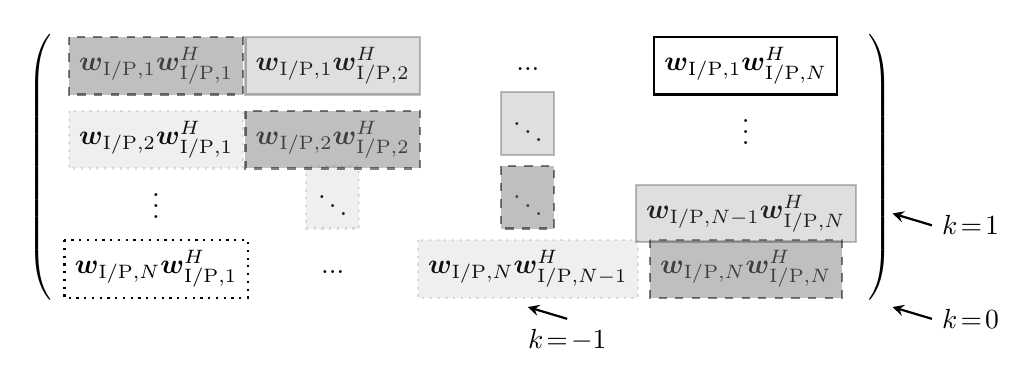
\begin{tikzpicture}[>=stealth,thick,baseline,every right delimiter/.append style={name=rd},]
						\matrix [matrix of math nodes,left delimiter=(,right delimiter=)] (m)
						{
							\boldsymbol{w}_{\mathrm{I/P},1}\boldsymbol{w}_{\mathrm{I/P},1}^H & \boldsymbol{w}_{\mathrm{I/P},1}\boldsymbol{w}_{\mathrm{I/P},2}^H & \dots & \boldsymbol{w}_{\mathrm{I/P},1}\boldsymbol{w}_{\mathrm{I/P},N}^H \\
							\boldsymbol{w}_{\mathrm{I/P},2}\boldsymbol{w}_{\mathrm{I/P},1}^H & \boldsymbol{w}_{\mathrm{I/P},2}\boldsymbol{w}_{\mathrm{I/P},2}^H & \ddots & \vdots \\
							\vdots & \ddots & \ddots & \boldsymbol{w}_{\mathrm{I/P},N-1}\boldsymbol{w}_{\mathrm{I/P},N}^H \\
							\boldsymbol{w}_{\mathrm{I/P},N}\boldsymbol{w}_{\mathrm{I/P},1}^H & \dots & \boldsymbol{w}_{\mathrm{I/P},N}\boldsymbol{w}_{\mathrm{I/P},N-1}^H & \boldsymbol{w}_{\mathrm{I/P},N}\boldsymbol{w}_{\mathrm{I/P},N}^H \\
						};
						\draw[dotted,thick] (m-4-1.north west) rectangle (m-4-1.south east);
						\draw[dotted,thick,fill=gray,opacity=0.125] (m-2-1.north west) rectangle (m-2-1.south east); \draw[dotted,thick,fill=gray,opacity=0.125] (m-3-2.north west) rectangle (m-3-2.south east); \draw[dotted,thick,fill=gray,opacity=0.125] (m-4-3.north west) rectangle (m-4-3.south east);
						\draw[dashed,thick,fill=gray,opacity=0.5] (m-1-1.north west) rectangle (m-1-1.south east); \draw[dashed,thick,fill=gray,opacity=0.5] (m-2-2.north west) rectangle (m-2-2.south east); \draw[dashed,thick,fill=gray,opacity=0.5] (m-3-3.north west) rectangle (m-3-3.south east); \draw[dashed,thick,fill=gray,opacity=0.5] (m-4-4.north west) rectangle (m-4-4.south east);
						\draw[solid,thick,fill=gray,opacity=0.25] (m-1-2.north west) rectangle (m-1-2.south east); \draw[solid,thick,fill=gray,opacity=0.25] (m-2-3.north west) rectangle (m-2-3.south east); \draw[solid,thick,fill=gray,opacity=0.25] (m-3-4.north west) rectangle (m-3-4.south east);
						\draw[solid,thick] (m-1-4.north west) rectangle (m-1-4.south east);
						\draw[<-] (m-4-3.south|-m.south) -- ++(0.5,-0.15) node[below]{$k=-1$};
						\draw[<-] (rd.east|-m.south) -- ++(0.5,-0.15) node[right]{$k=0$};
						\draw[<-] (rd.east|-m-3-4.east) -- ++(0.5,-0.15) node[right]{$k=1$};
					\end{tikzpicture}
				\end{equation*}
				\caption{$\boldsymbol{W}_{\mathrm{I/P}}$ consists of $N \times N$ blocks of size $M \times M$. $\boldsymbol{W}_{\mathrm{I/P},k}$ keeps the $k$-th block diagonal of $\boldsymbol{W}_{\mathrm{I/P}}$ and nulls all remaining blocks. Solid, dashed and dotted blocks correspond to $k>0$, $k=0$ and $k<0$, respectively. For $\boldsymbol{w}_{\mathrm{I/P},n_1}\boldsymbol{w}_{\mathrm{I/P},n_2}^H$, the $k$-th block diagonal satisfies $k=n_2-n_1$.}
				\label{fi:block_diagonal}
			\end{figure*}

			\begin{figure*}[!b]
				\hrule
				\begin{align}
					&z(\boldsymbol{\phi},\boldsymbol{w}_{\mathrm{I}},\boldsymbol{w}_{\mathrm{P}},\rho) = \beta_2\rho\Bigl(\mathbb{E}\left\{\mathbb{A}\left\{y_{\mathrm{I}}^2(t)\right\}\right\}+\mathbb{A}\left\{y_{\mathrm{P}}^2(t)\right\}\Bigr)+\beta_4\rho^2\Bigl(\mathbb{E}\left\{\mathbb{A}\left\{y_{\mathrm{I}}^4(t)\right\}\right\}+\mathbb{A}\left\{y_{\mathrm{P}}^4(t)\right\}+6\mathbb{E}\left\{\mathbb{A}\left\{y_{\mathrm{I}}^2(t)\right\}\right\}\mathbb{A}\left\{y_{\mathrm{P}}^2(t)\right\}\Bigr),\label{eq:z_expand}\\
					&\mathbb{E}\left\{\mathbb{A}\left\{y_{\mathrm{I}}^2(t)\right\}\right\} = \frac{1}{2}\sum_{n=1}^N{(\boldsymbol{h}_{n}^H\boldsymbol{w}_{\mathrm{I},n})(\boldsymbol{h}_{n}^H\boldsymbol{w}_{\mathrm{I},n})^*} = \frac{1}{2}\boldsymbol{h}^H\boldsymbol{W}_{\mathrm{I},0}\boldsymbol{h},\label{eq:y_I2}\\
					&\mathbb{E}\left\{\mathbb{A}\left\{y_{\mathrm{I}}^4(t)\right\}\right\} = \frac{3}{4}\left(\sum_{n=1}^N{(\boldsymbol{h}_{n}^H\boldsymbol{w}_{\mathrm{I},n})(\boldsymbol{h}_{n}^H\boldsymbol{w}_{\mathrm{I},n})^*}\right)^2 = \frac{3}{4}(\boldsymbol{h}^H\boldsymbol{W}_{\mathrm{I},0}\boldsymbol{h})^2,\label{eq:y_I4}\\
					&\mathbb{A}\left\{y_{\mathrm{P}}^2(t)\right\} = \frac{1}{2}\sum_{n=1}^N{(\boldsymbol{h}_{n}^H\boldsymbol{w}_{\mathrm{P},n})(\boldsymbol{h}_{n}^H\boldsymbol{w}_{\mathrm{P},n})^*} = \frac{1}{2}\boldsymbol{h}^H\boldsymbol{W}_{\mathrm{P},0}\boldsymbol{h},\label{eq:y_P2}\\
					&\mathbb{A}\left\{y_{\mathrm{P}}^4(t)\right\} = \frac{3}{8}\sum_{\substack{{n_1},{n_2},{n_3},{n_4}\\{n_1}+{n_2}={n_3}+{n_4}}}{(\boldsymbol{h}_{{n_1}}^H\boldsymbol{w}_{\mathrm{P},{n_1}})(\boldsymbol{h}_{{n_2}}^H\boldsymbol{w}_{\mathrm{P},{n_2}})(\boldsymbol{h}_{{n_3}}^H\boldsymbol{w}_{\mathrm{P},{n_3}})^*(\boldsymbol{h}_{{n_4}}^H\boldsymbol{w}_{\mathrm{P},{n_4}})^*} = \frac{3}{8}\sum_{k=-N+1}^{N-1}(\boldsymbol{h}^H\boldsymbol{W}_{\mathrm{P},k}\boldsymbol{h})(\boldsymbol{h}^H\boldsymbol{W}_{\mathrm{P},k}\boldsymbol{h})^*.\label{eq:y_P4}
				\end{align}
			\end{figure*}
		\end{subsection}


		\begin{subsection}{Rate-Energy Region}
			The achievable R-E region is defined as
			\begin{align}
				\mathcal{C}_{\mathrm{R-E}}
				&\triangleq \biggl\{(R_{\mathrm{ID}}, z_{\mathrm{EH}}) \in \mathbb{R}_+^2 \mid R_{\mathrm{ID}} \le R, z_{\mathrm{EH}} \le z,\nonumber\\
				&\quad \frac{1}{2}\left(\lVert{\boldsymbol{w}_{\mathrm{I}}}\rVert^2+\lVert{\boldsymbol{w}_{\mathrm{P}}}\rVert^2\right) \le P\biggr\},
			\end{align}
			where $P$ is the average transmit power budget and \num{1/2} converts the peak value of the sine waves to the average value.
		\end{subsection}
	\end{section}


	\begin{section}{Problem Formulation}\label{se:problem_formulation}
		We characterize each R-E boundary point through a current maximization problem subject to sum rate, transmit power, and IRS magnitude constraints as
		\begin{maxi!}
			{\scriptstyle{\boldsymbol{\phi},\boldsymbol{w}_{\mathrm{I}},\boldsymbol{w}_{\mathrm{P}},\rho}}{z(\boldsymbol{\phi},\boldsymbol{w}_{\mathrm{I}},\boldsymbol{w}_{\mathrm{P}},\rho)}{\label{op:original}}{\label{ob:original}}
			\addConstraint{R(\boldsymbol{\phi},\boldsymbol{w}_{\mathrm{I}},\rho) \ge \bar{R}}\label{co:original_rate}
			\addConstraint{\frac{1}{2}\left(\lVert{\boldsymbol{w}_{\mathrm{I}}}\rVert^2+\lVert{\boldsymbol{w}_{\mathrm{P}}}\rVert^2\right)\le{P}}\label{co:original_power}
			\addConstraint{\lvert{\boldsymbol{\phi}}\rvert=\boldsymbol{1}}\label{co:original_modulus}
			\addConstraint{0 \le \rho \le 1.}
		\end{maxi!}
		Problem~\eqref{op:original} is intricate due to the coupled variables in \eqref{ob:original}, \eqref{co:original_rate} and the non-convex constraint \eqref{co:original_modulus}. To obtain a feasible solution, we propose a BCD algorithm that iteratively updates 1) the IRS phase shift; 2) the active precoder; 3) the waveform amplitude and splitting ratio, until convergence.


		\begin{subsection}{Passive Beamforming}
			In this section, we optimize the IRS phase shift $\boldsymbol{\phi}$ for any given waveform $\boldsymbol{w}_{\mathrm{I/P}}$ and splitting ratio $\rho$. Note that
			\begin{align}
				\lvert \boldsymbol{h}_{n}^H\boldsymbol{w}_{\mathrm{I},n} \rvert^2
				& = \boldsymbol{w}_{\mathrm{I},n}^H\boldsymbol{h}_n\boldsymbol{h}_n^H\boldsymbol{w}_{\mathrm{I},n}\nonumber\\
				& = \boldsymbol{w}_{\mathrm{I},n}^H(\boldsymbol{h}_{\mathrm{D},n}+\boldsymbol{V}_n^H\boldsymbol{\phi})(\boldsymbol{h}_{\mathrm{D},n}^H+\boldsymbol{\phi}^H\boldsymbol{V}_n)\boldsymbol{w}_{\mathrm{I},n}\nonumber\\
				& = \boldsymbol{w}_{\mathrm{I},n}^H\boldsymbol{M}_n^H\boldsymbol{\Phi}\boldsymbol{M}_n\boldsymbol{w}_{\mathrm{I},n}\nonumber\\
				& = \mathrm{tr}(\boldsymbol{M}_n\boldsymbol{w}_{\mathrm{I},n}\boldsymbol{w}_{\mathrm{I},n}^H\boldsymbol{M}_n^H\boldsymbol{\Phi})\nonumber\\
				& = \mathrm{tr}(\boldsymbol{C}_n\boldsymbol{\Phi}),
			\end{align}
			where $\boldsymbol{M}_n \triangleq [\boldsymbol{V}_n^H, \boldsymbol{h}_{\mathrm{D},n}]^H \in \mathbb{C}^{(L+1) \times M}$, $t'$ is an auxiliary variable with unit modulus, $\bar{\boldsymbol{\phi}} \triangleq [\boldsymbol{\phi}^H, t']^H \in \mathbb{C}^{(L+1) \times 1}$, $\boldsymbol{\Phi} \triangleq \bar{\boldsymbol{\phi}}\bar{\boldsymbol{\phi}}^H \in \mathbb{C}^{(L+1) \times (L+1)}$, $\boldsymbol{C}_n \triangleq \boldsymbol{M}_n\boldsymbol{w}_{\mathrm{I},n}\boldsymbol{w}_{\mathrm{I},n}^H\boldsymbol{M}_n^H \in \mathbb{C}^{(L+1)\times(L+1)}$. On the other hand, we define $t_{\mathrm{I/P},k}$ as
			\begin{align}
				t_{\mathrm{I/P},k}
				& \triangleq \boldsymbol{h}^H\boldsymbol{W}_{\mathrm{I/P},k}\boldsymbol{h}\nonumber\\
				& = \mathrm{tr}(\boldsymbol{h}\boldsymbol{h}^H\boldsymbol{W}_{\mathrm{I/P},k})\nonumber\\
				& = \mathrm{tr}\left((\boldsymbol{h}_{D}+\boldsymbol{V}^H\boldsymbol{\phi})(\boldsymbol{h}_{D}^H+\boldsymbol{\phi}^H\boldsymbol{V})\boldsymbol{W}_{\mathrm{I/P},k}\right)\nonumber\\
				& = \mathrm{tr}(\boldsymbol{M}^H\boldsymbol{\Phi}\boldsymbol{M}\boldsymbol{W}_{\mathrm{I/P},k})\nonumber\\
				& = \mathrm{tr}(\boldsymbol{M}\boldsymbol{W}_{\mathrm{I/P},k}\boldsymbol{M}^H\boldsymbol{\Phi})\nonumber\\
				& = \mathrm{tr}(\boldsymbol{C}_{\mathrm{I/P},k}\boldsymbol{\Phi})\label{eq:t_k},
			\end{align}
			where $\boldsymbol{V} \triangleq [\boldsymbol{V}_1,\dots,\boldsymbol{V}_N] \in \mathbb{C}^{L \times MN}$, $\boldsymbol{M} \triangleq [\boldsymbol{V}^H, \boldsymbol{h}_{D}]^H \in \mathbb{C}^{(L+1) \times MN}$, $\boldsymbol{C}_{\mathrm{I/P},k} \triangleq \boldsymbol{M}\boldsymbol{W}_{\mathrm{I/P},k}\boldsymbol{M}^H \in \mathbb{C}^{(L+1)\times(L+1)}$. On top of this, \eqref{eq:R} and \eqref{eq:z_expand} reduce respectively to
			\begin{align}
				R(\boldsymbol{\Phi})
				& = \sum_{n=1}^{N}{\log_2\left(1+\frac{(1-\rho)\mathrm{tr}(\boldsymbol{C}_n\boldsymbol{\Phi})}{\sigma_n^2}\right)},\label{eq:R_irs}\\
				z(\boldsymbol{\Phi})
				& = \frac{1}{2}{\beta_2}{\rho}(t_{\mathrm{I},0}+t_{\mathrm{P},0}) + \frac{3}{8}{\beta_4}{\rho^2} \left(2t_{\mathrm{I},0}^2 + \sum_{k=-N+1}^{N-1}{t_{\mathrm{P},k}t_{\mathrm{P},k}^*}\right)\nonumber\\
				& \quad + \frac{3}{2}{\beta_4}{\rho^2}t_{\mathrm{I},0}t_{\mathrm{P},0}.\label{eq:z_irs}
			\end{align}
			To maximize the non-concave expression \eqref{eq:z_irs}, we successively lower bound the second-order terms by their first-order Taylor expansions \cite{Adali2010}. Based on the solution at iteration $i - 1$, the approximations at iteration $i$ are
			\begin{align}
				(t_{\mathrm{I},0}^{(i)})^2
				& \ge 2 t_{\mathrm{I},0}^{(i)}t_{\mathrm{I},0}^{(i-1)} - (t_{\mathrm{I},0}^{(i-1)})^2,\label{eq:taylor_1}\\
				t_{\mathrm{P},k}^{(i)} (t_{\mathrm{P},k}^{(i)})^*
				& \ge 2 \Re\left\{t_{\mathrm{P},k}^{(i)} (t_{\mathrm{P},k}^{(i-1)})^*\right\} - t_{\mathrm{P},k}^{(i-1)} (t_{\mathrm{P},k}^{(i-1)})^*,\label{eq:taylor_2}\\
				t_{\mathrm{I},0}^{(i)} t_{\mathrm{P},0}^{(i)}
				& \ge t_{\mathrm{I},0}^{(i)} t_{\mathrm{P},0}^{(i-1)} + t_{\mathrm{P},0}^{(i)} t_{\mathrm{I},0}^{(i-1)} - t_{\mathrm{I},0}^{(i-1)} t_{\mathrm{P},0}^{(i-1)}.\label{eq:taylor_3}
			\end{align}
			Note that $t_{\mathrm{I/P},0}=\mathrm{tr}(\boldsymbol{C}_{\mathrm{I/P},0}\boldsymbol{\Phi})$ is real-valued because $\boldsymbol{C}_{\mathrm{I/P},0}$ and $\boldsymbol{\Phi}$ are Hermitian matrices. Due to symmetry \cite{Golub2013}, we have
			\begin{equation}\label{eq:coupled_terms}
				\sum_{k=-N+1}^{N-1} \Re\left\{t_{\mathrm{P},k}^{(i)} (t_{\mathrm{P},k}^{(i-1)})^*\right\} = \sum_{k=-N+1}^{N-1} t_{\mathrm{P},k}^{(i)} (t_{\mathrm{P},k}^{(i-1)})^*.
			\end{equation}
			Plugging \eqref{eq:taylor_1}--\eqref{eq:coupled_terms} into \eqref{eq:z_irs}, we obtain the DC current approximation $\tilde{z}$ as \eqref{eq:z_irs_approx} and transform problem~\eqref{op:original} to
			\begin{figure*}[!b]
				\hrule
				\begin{align}
					\tilde{z}(\boldsymbol{\Phi}^{(i)})
					& = \frac{1}{2}{\beta_2}{\rho}(t_{\mathrm{I},0}^{(i)}+t_{\mathrm{P},0}^{(i)}) + \frac{3}{8}{\beta_4}{\rho^2} \left(4 t_{\mathrm{I},0}^{(i)}t_{\mathrm{I},0}^{(i-1)} - 2 (t_{\mathrm{I},0}^{(i-1)})^2 + \sum_{k=-N+1}^{N-1}{2 t_{\mathrm{P},k}^{(i)} (t_{\mathrm{P},k}^{(i-1)})^* - t_{\mathrm{P},k}^{(i-1)} (t_{\mathrm{P},k}^{(i-1)})^*}\right)\nonumber\\
					& \quad + \frac{3}{2}{\beta_4}{\rho^2} \left(t_{\mathrm{I},0}^{(i)} t_{\mathrm{P},0}^{(i-1)} + t_{\mathrm{P},0}^{(i)} t_{\mathrm{I},0}^{(i-1)} - t_{\mathrm{I},0}^{(i-1)} t_{\mathrm{P},0}^{(i-1)}\right).\label{eq:z_irs_approx}
				\end{align}
			\end{figure*}
			\begin{maxi!}
				{\scriptstyle{\boldsymbol{\Phi}}}{\tilde{z}(\boldsymbol{\Phi})}{\label{op:irs}}{\label{ob:irs}}
				\addConstraint{R(\boldsymbol{\Phi}) \ge \bar{R}}\label{co:irs_rate}
				\addConstraint{\mathrm{diag}^{-1}(\boldsymbol{\Phi})=\boldsymbol{1}}\label{co:irs_modulus}
				\addConstraint{\boldsymbol{\Phi}\succeq{\boldsymbol{0}}}\label{co:irs_sd}
				\addConstraint{\mathrm{rank}(\boldsymbol{\Phi})=1.\label{co:irs_rank}}
			\end{maxi!}
			We then apply Semi-Definite Relaxation (SDR) to the unit-rank constraint \eqref{co:irs_rank} and formulate a Semi-Definite Programming (SDP) with approximation accuracy no greater than $\pi/4$ \cite{Luo2010}. In this specific case, we found the solution provided by CVX toolbox \cite{Grant2008} to \eqref{ob:irs}-\eqref{co:irs_sd} is always rank-\num{1}. This conclusion is summarized below.

			\begin{proposition}\label{pr:relaxation}
				Any optimal solution $\boldsymbol{\Phi}^\star$ to the relaxed passive beamforming problem~\eqref{ob:irs}--\eqref{co:irs_sd} is rank-\num{1} such that \eqref{co:irs_rank} is tight and no loss is introduced by SDR.
			\end{proposition}

			\begin{proof}\label{pf:relaxation}
				Please refer to Appendix~\ref{ap:relaxation}.
			\end{proof}

			In summary, we update $\boldsymbol{\Phi}^{(i)}$ until convergence, extract $\hat{\boldsymbol{\phi}}^\star$ by eigen decomposition, and retrieve the	IRS vector by $\boldsymbol{\phi}^{\star}=e^{j \arg\left([\hat{\boldsymbol{\phi}}^\star]_{(1:L)} \middle/ [\hat{\boldsymbol{\phi}}^\star]_{(L+1)}\right)}$. The passive beamforming design is summarized in the SCA Algorithm~\ref{al:sca}, where the relaxed problem \eqref{ob:irs}--\eqref{co:irs_sd} involves a $(L+1)$-order positive semi-definite matrix variable and $(L+2)$ linear constraints. Given a solution accuracy $\epsilon_{\mathrm{IPM}}$ for the interior-point method, the computational complexity of Algorithm~\ref{al:sca} is $\mathcal{O}\left(I_{\mathrm{SCA}}(L+2)^4 (L+1)^{0.5} \log(\epsilon_{\mathrm{IPM}}^{-1})\right)$, where $I_{\mathrm{SCA}}$ denotes the number of SCA iterations \cite{Luo2010}.

			\begin{algorithm}[!t]
				\caption{SCA: IRS Phase Shift.}
				\label{al:sca}
				\begin{algorithmic}[1]
					\State \textbf{Input} $\beta_2$, $\beta_4$, $\boldsymbol{h}_{\mathrm{D},n}$, $\boldsymbol{V}_{n}$, $\sigma_n$, $\boldsymbol{w}_{\mathrm{I/P},n}$, $\rho$, $\bar{R}$, $\epsilon$, $\forall n$
					\State Construct $\boldsymbol{V}$, $\boldsymbol{M}$, $\boldsymbol{M}_n$, $\boldsymbol{C}_{n}$, $\boldsymbol{C}_{\mathrm{I/P},k}$, $\forall n,k$
					\State \textbf{Initialize} $i \gets 0$, $\boldsymbol{\Phi}^{(0)}$
					\State Set $t_{\mathrm{I/P},k}^{(0)}$, $\forall k$ by \eqref{eq:t_k}
					\State Compute $z^{(0)}$ by \eqref{eq:z_irs}
					\Repeat
						\State $i \gets i + 1$
						\State Get $\boldsymbol{\Phi}^{(i)}$ by solving \eqref{ob:irs}--\eqref{co:irs_sd}
						\State Update $t_{\mathrm{I/P},k}^{(i)}$, $\forall k$ by \eqref{eq:t_k}
						\State Compute $z^{(i)}$ by \eqref{eq:z_irs}
					\Until $\lvert z^{(i)}-z^{(i-1)} \rvert \le \epsilon$
					\State Set $\boldsymbol{\Phi}^{\star} \gets \boldsymbol{\Phi}^{(i)}$
					\State Get $\hat{\boldsymbol{\phi}}^\star$ by eigen decomposition, $\boldsymbol{\Phi}^{\star}=\hat{\boldsymbol{\phi}}^\star(\hat{\boldsymbol{\phi}}^\star)^H$
					\State Set $\boldsymbol{\phi}^{\star} \gets e^{j \arg\left([\hat{\boldsymbol{\phi}}^\star]_{(1:L)} \middle/ [\hat{\boldsymbol{\phi}}^\star]_{(L+1)}\right)}$
					\State \textbf{Output} $\boldsymbol{\phi}^{\star}$
				\end{algorithmic}
			\end{algorithm}

			\begin{proposition}\label{pr:sca}
				For any feasible initial point with given waveform and splitting ratio, the SCA Algorithm~\ref{al:sca} is guaranteed to converge to local optimal points of the original problem~\eqref{op:original}.
			\end{proposition}

			\begin{proof}\label{pf:sca}
				Please refer to Appendix~\ref{ap:sca}.
			\end{proof}
		\end{subsection}

		\begin{subsection}{Active Beamforming}
			To avoid straightforward optimization over complex vectors $\boldsymbol{w}_{\mathrm{I/P}}$ of size $MN \times 1$, we decouple the waveform in the spatial and frequency domains to reduce the size of variables. The weight on subband $n$ is essentially
			\begin{equation}\label{eq:w}
				\boldsymbol{w}_{\mathrm{I/P}, n} = s_{\mathrm{I/P}, n} \boldsymbol{b}_{\mathrm{I/P}, n},
			\end{equation}
			where $s_{\mathrm{I/P},n}$ denotes the amplitude of the modulated/multisine waveform at tone $n$, and $\boldsymbol{b}_{\mathrm{I/P}, n}$ denotes the corresponding information/power precoder. Define $\boldsymbol{s}_{\mathrm{I/P}} \triangleq [s_{\mathrm{I/P},1},\dots,s_{\mathrm{I/P},N}]^T \in \mathbb{R}_+^{N \times 1}$. The MRT precoder at subband $n$ is given by
			\begin{equation}\label{eq:b_n}
				\boldsymbol{b}_{\mathrm{I/P}, n}^\star = \frac{\boldsymbol{h}_n}{\lVert{\boldsymbol{h}_n}\rVert}.
			\end{equation}

			\begin{proposition}\label{pr:mrt}
				For single-user SWIPT, the global optimal information and power precoders coincide at the MRT.
			\end{proposition}

			\begin{proof}\label{pf:mrt}
				Please refer to Appendix~\ref{ap:mrt}.
			\end{proof}
		\end{subsection}


		\begin{subsection}{Waveform and Splitting Ratio}
			Next, we jointly optimize the waveform amplitude $\boldsymbol{s}_{\mathrm{I/P}}$ and the splitting ratio $\rho$ for any given IRS phase shift $\boldsymbol{\phi}$ and active precoder $\boldsymbol{b}_{\mathrm{I/P},n}$, $\forall n$. On top of \eqref{eq:b_n}, the equivalent channel strength at subband $n$ is $\lVert{\boldsymbol{h}_n}\rVert$. Hence, the rate \eqref{eq:R} reduces to
			\begin{equation}\label{eq:R_waveform}
				R(\boldsymbol{s}_{\mathrm{I}},\rho) = \log_2\prod_{n=1}^N\left(1+\frac{(1-\rho)\lVert{\boldsymbol{h}_n}\rVert^2 s_{\mathrm{I},n}^2}{\sigma_n^2}\right),
			\end{equation}
			and the DC current \eqref{eq:z_expand} rewrites as \eqref{eq:z_waveform}, so that problem~\eqref{op:original} boils down to
			\begin{figure*}[!b]
				\hrule
				\begin{align}
					z(\boldsymbol{s}_{\mathrm{I}},\boldsymbol{s}_\mathrm{P},\rho)
					& = \frac{1}{2}{\beta_2}{\rho} \sum_{n=1}^N \lVert{\boldsymbol{h}_n}\rVert^2(s_{\mathrm{I},n}^2+s_{\mathrm{P},n}^2) + \frac{3}{8}{\beta_4}{\rho^2} \left( 2\sum_{n_1,n_2} \prod_{j=1}^2 \lVert{\boldsymbol{h}_{n_j}}\rVert^2 s_{\mathrm{I},{n_j}}^2 + \sum_{\substack{{n_1},{n_2},{n_3},{n_4}\\{n_1}+{n_2}={n_3}+{n_4}}} \prod_{j=1}^4 \lVert{\boldsymbol{h}_{n_j}}\rVert s_{\mathrm{P},{n_j}} \right)\nonumber\\
					& \quad + \frac{3}{2}{\beta_4}{\rho^2} \left( \sum_{n_1,n_2} \lVert{\boldsymbol{h}_{n_1}}\rVert^2 \lVert{\boldsymbol{h}_{n_2}}\rVert^2 s_{\mathrm{I},{n_1}}^2 s_{\mathrm{P},{n_2}}^2 \right).\label{eq:z_waveform}
				\end{align}
			\end{figure*}
			\begin{maxi!}
				{\scriptstyle{\boldsymbol{s}_{\mathrm{I}},\boldsymbol{s}_\mathrm{P},\rho}}{z(\boldsymbol{s}_{\mathrm{I}},\boldsymbol{s}_\mathrm{P},\rho)}{\label{op:waveform}}{}
				\addConstraint{R(\boldsymbol{s}_{\mathrm{I}},\rho) \ge \bar{R}}
				\addConstraint{\frac{1}{2}\left(\lVert{\boldsymbol{s}_{\mathrm{I}}}\rVert^2+\lVert{\boldsymbol{s}_\mathrm{P}}\rVert^2\right)\le{P}.}
			\end{maxi!}
			Following \cite{Clerckx2018b}, we introduce auxiliary variables $t'',\bar{\rho}$ and transform problem~\eqref{op:waveform} into a reversed GP\footnote{It can be concluded $\bar{\rho}^{\star}=1-\rho^{\star}$ as no signal is wasted at the receiver.}
			\begin{mini!}
				{\scriptstyle{\boldsymbol{s}_{\mathrm{I}},\boldsymbol{s}_\mathrm{P},\rho,\bar{\rho},t''}}{\frac{1}{t''}}{\label{op:waveform_rgp}}{}
				\addConstraint{\frac{t''}{z(\boldsymbol{s}_{\mathrm{I}},\boldsymbol{s}_\mathrm{P},\rho)} \le 1}\label{co:waveform_objective}
				\addConstraint{\frac{2^{\bar{R}}}{\prod_{n=1}^N \left(1+{\bar{\rho}\lVert{\boldsymbol{h}_n}\rVert^2 s_{\mathrm{I},n}^2}\big/{\sigma_n^2}\right)} \le 1}\label{co:waveform_rate}
				\addConstraint{\frac{1}{2}\left(\lVert{\boldsymbol{s}_{\mathrm{I}}}\rVert^2+\lVert{\boldsymbol{s}_\mathrm{P}}\rVert^2\right) \le P}\label{co:waveform_power}
				\addConstraint{\rho + \bar{\rho} \le 1.}\label{co:waveform_splitting_ratio}
			\end{mini!}
			The denominators of \eqref{co:waveform_rate} and \eqref{co:waveform_objective} consist of posynomials \cite{Boyd2007} that can be decomposed as sums of monomials
			\begin{align}
				1+\frac{\bar{\rho}\lVert{\boldsymbol{h}_n}\rVert^2 s_{\mathrm{I},n}^2}{\sigma_n^2} &\triangleq \sum_{m_{\mathrm{I},n}}g_{m_{\mathrm{I},n}}(s_{\mathrm{I},n},\bar{\rho})\label{eq:g_I},\\
				z(\boldsymbol{s}_{\mathrm{I}},\boldsymbol{s}_\mathrm{P},\rho) &\triangleq \sum_{m_\mathrm{P}}{g_{m_\mathrm{P}}(\boldsymbol{s}_{\mathrm{I}},\boldsymbol{s}_\mathrm{P},\rho)}\label{eq:g_P}.
			\end{align}
			We upper bound \eqref{eq:g_I} and \eqref{eq:g_P} by the Arithmetic Mean-Geometric Mean (AM-GM) inequality \cite{Chiang2005} and transform problem~\eqref{op:waveform_rgp} to
			\begin{mini!}
				{\scriptstyle{\boldsymbol{s}_{\mathrm{I}},\boldsymbol{s}_\mathrm{P},\rho,\bar{\rho},t''}}{\frac{1}{t''}}{\label{op:waveform_gp}}{}
				\addConstraint{{t''}\prod_{m_\mathrm{P}}{\left(\frac{g_{{m_\mathrm{P}}}(\boldsymbol{s}_{\mathrm{I}},\boldsymbol{s}_\mathrm{P},\rho)}{\gamma_{{m_\mathrm{P}}}}\right)^{-\gamma_{{m_\mathrm{P}}}}}\le{1}}
				\addConstraint{2^{\bar{R}}\prod_{n}\prod_{m_{\mathrm{I},n}}\left(\frac{g_{m_{\mathrm{I},n}}(s_{\mathrm{I},n},\bar{\rho})}{\gamma_{m_{\mathrm{I},n}}}\right)^{-\gamma_{m_{\mathrm{I},n}}}\le{1}}
				\addConstraint{\frac{1}{2}\left(\lVert{\boldsymbol{s}_{\mathrm{I}}}\rVert^2+\lVert{\boldsymbol{s}_\mathrm{P}}\rVert^2\right)\le{P}}
				\addConstraint{\rho + \bar{\rho} \le 1,}
			\end{mini!}
			where $\gamma_{m_{\mathrm{I},n}},\gamma_{m_\mathrm{P}} \ge 0$ and $\sum_{m_{\mathrm{I},n}}\gamma_{m_{\mathrm{I},n}}=\sum_{m_\mathrm{P}}\gamma_{m_\mathrm{P}}=1$. The tightness of the AM-GM inequality depends on $\{\gamma_{m_{\mathrm{I},n}},\gamma_{m_\mathrm{P}}\}$, and a feasible choice at iteration $i$ is
			\begin{align}
				\gamma_{m_{\mathrm{I},n}}^{(i)} & = \frac{g_{m_{\mathrm{I},n}}(s_{\mathrm{I},n}^{(i-1)},\bar{\rho}^{(i-1)})}{1+{\bar{\rho}^{(i-1)}\lVert{\boldsymbol{h}_n}\rVert^2 (s_{\mathrm{I},n}^{(i-1)})^2}\big/{\sigma_n^2}}\label{eq:gamma_I},\\
				\gamma_{m_\mathrm{P}}^{(i)} & = \frac{g_{m_\mathrm{P}}(\boldsymbol{s}_{\mathrm{I}}^{(i-1)},\boldsymbol{s}_\mathrm{P}^{(i-1)},\rho^{(i-1)})}{z(\boldsymbol{s}_{\mathrm{I}}^{(i-1)},\boldsymbol{s}_\mathrm{P}^{(i-1)},\rho^{(i-1)})}\label{eq:gamma_P}.
			\end{align}
			With \eqref{eq:gamma_I} and \eqref{eq:gamma_P}, problem~\eqref{op:waveform_gp} can be solved by existing optimization tools such as CVX \cite{Grant2008}. We update $\boldsymbol{s}_{\mathrm{I}}^{(i)},\boldsymbol{s}_\mathrm{P}^{(i)},\rho^{(i)}$ iteratively until convergence. The joint waveform amplitude and splitting ratio design is summarized in the GP Algorithm~\ref{al:gp}, which achieves local optimality at the cost of exponential computational complexity \cite{Chiang2005}.

			\begin{algorithm}[!t]
				\caption{GP: Waveform Amplitude and Splitting Ratio.}
				\label{al:gp}
				\begin{algorithmic}[1]
					\State \textbf{Input} $\beta_2$, $\beta_4$, $\boldsymbol{h}_n$, $P$, $\sigma_n$, $\bar{R}$, $\epsilon$, $\forall n$
					\State \textbf{Initialize} $i \gets 0$, $\boldsymbol{s}_{\mathrm{I/P}}^{(0)}$, $\rho^{(0)}$
					\State Compute $R^{(0)}$, $z^{(0)}$ by \eqref{eq:R_waveform}, \eqref{eq:z_waveform}
					\State Set $g_{m_{\mathrm{I},n}}^{(0)}$, $g_{m_\mathrm{P}}^{(0)}$, $\forall n$ by \eqref{eq:g_I}, \eqref{eq:g_P}
					\Repeat
						\State $i \gets i + 1$
						\State Update $\gamma_{m_{\mathrm{I},n}}^{(i)}$, $\gamma_{m_\mathrm{P}}^{(i)}$, $\forall n$ by \eqref{eq:gamma_I}, \eqref{eq:gamma_P}
						\State Get $\boldsymbol{s}_{\mathrm{I/P}}^{(i)}$, $\rho^{(i)}$ by solving problem~\eqref{op:waveform_gp}
						\State Compute $R^{(i)}$, $z^{(i)}$ by \eqref{eq:R_waveform}, \eqref{eq:z_waveform}
						\State Update $g_{m_{\mathrm{I},n}}^{(i)}$, $g_{m_\mathrm{P}}^{(i)}$, $\forall n$ by \eqref{eq:g_I}, \eqref{eq:g_P}
					\Until $\lvert z^{(i)} - z^{(i-1)} \rvert \le \epsilon$
					\State Set $\boldsymbol{s}_{\mathrm{I/P}}^{\star} \gets \boldsymbol{s}_{\mathrm{I/P}}^{(i)}$, $\rho^{\star} \gets \rho^{(i)}$
					\State \textbf{Output} $\boldsymbol{s}_{\mathrm{I}}^{\star}$, $\boldsymbol{s}_{\mathrm{P}}^{\star}$, $\rho^{\star}$
				\end{algorithmic}
			\end{algorithm}

			\begin{proposition}\label{pr:gp}
				For any feasible initial point, the GP Algorithm~\ref{al:gp} is guaranteed to converge to local optimal points of the waveform amplitude and splitting ratio design problem \eqref{op:waveform}.
			\end{proposition}

			\begin{proof}\label{pf:gp}
				Please refer to \cite{Clerckx2016a,Clerckx2018b}.
			\end{proof}
		\end{subsection}


		\begin{subsection}{Low-Complexity Adaptive Design}
			To facilitate practical SWIPT implementation, we propose two closed-form adaptive waveform amplitude schemes by combining WF and SMF in the time and power domains. For WIT, the optimal WF strategy assigns the amplitude of modulated tone $n$ by
			\begin{equation}\label{eq:wf}
				s_{\mathrm{I}, n} = \sqrt{2\left(\lambda - \frac{\sigma_n^2}{P \lVert{\boldsymbol{h}_n}\rVert^2}\right)^+},
			\end{equation}
			where $\lambda$ is chosen to satisfy the power constraint $\lVert{\boldsymbol{s}_I}\rVert^2 / 2 \le P$. The closed-form solution can be obtained by iterative power allocation \cite{Tse2005}, and the details are omitted here. On the other hand, SMF was proposed in \cite{Clerckx2017} as a suboptimal WPT resource allocation scheme that assigns the amplitude of sinewave $n$ by
			\begin{equation}\label{eq:smf}
				s_{\mathrm{P}, n} = \sqrt{\frac{2 P}{\sum_{n=1}^N \lVert{\boldsymbol{h}_n \rVert^{2 \alpha}}}}\lVert{\boldsymbol{h}_n}\rVert^\alpha,
			\end{equation}
			where the scaling ratio $\alpha \ge 1$ is predetermined to exploit the rectifier nonlinearity and frequency selectivity. When the receiver works in TS mode, there is no superposition in the suboptimal waveform design. Modulated waveform with amplitude \eqref{eq:wf} is used in the data session while multisine waveform with amplitude \eqref{eq:smf} is used in the energy session. When the receiver works in PS mode, we jointly design the combining ratio $\delta$ with the splitting ratio $\rho$, and assign the superposed waveform amplitudes as
			\begin{align}
				s_{\mathrm{I}, n} &= \sqrt{2(1 - \delta)\left(\lambda - \frac{\sigma_n^2}{P \lVert{\boldsymbol{h}_n}\rVert^2}\right)^+}, \label{eq:s_i}\\
				s_{\mathrm{P}, n} &= \sqrt{\frac{2 \delta P}{\sum_{n=1}^N \lVert{\boldsymbol{h}_n \rVert^{2 \alpha}}}}\lVert{\boldsymbol{h}_n}\rVert^\alpha, \label{eq:s_p}
			\end{align}
			where the combining ratio $\delta$ determines the priority of multisine waveform at the transmitter and the splitting ratio $\rho$ determines the priority of the energy harvester at the receiver.\footnote{We notice that $\delta^{\star}=\rho^{\star}=0$ at the WIT point and $\delta^{\star}=\rho^{\star}=1$ at the WPT point when $N$ is relatively large. Heuristically, $\delta^{\star}$ and $\rho^{\star}$ should approximately equal at each point to boost R-E tradeoff.}

			Besides, minor modifications are required for passive beamforming to accommodate the low-complexity waveform schemes. The rate constraint \eqref{co:irs_rate} should be dropped as the achievable rate is controlled by $\eta$ or $\{\delta,\rho\}$. To achieve the WIT point ($\rho=0$), the rate \eqref{eq:R_irs} should be maximized, the current expression \eqref{eq:z_irs_approx} should be dropped, and no SCA is involved. The Modified-SCA (M-SCA) Algorithm~\ref{al:m_sca} summarizes the modified passive beamforming design when the receiver works in PS mode. Similarly, no loss is introduced by SDR and local optimality is guaranteed, and the proofs are omitted. Since each SDP involves $(L+1)$ linear constraints, the computational complexity of Algorithm~\ref{al:m_sca} is $\mathcal{O}\left(I_{\mathrm{M-SCA}}(L+1)^{4.5} \log(\epsilon_{\mathrm{IPM}}^{-1})\right)$, where $I_{\mathrm{M-SCA}}$ denotes the number of M-SCA iterations \cite{Luo2010}. Note that no SCA is involved at the WIT point where $I_{\mathrm{M-SCA}}=1$.

			\begin{algorithm}[!t]
				\caption{M-SCA: IRS Phase Shift.}
				\label{al:m_sca}
				\begin{algorithmic}[1]
					\State \textbf{Input} $\beta_2$, $\beta_4$, $\boldsymbol{h}_{\mathrm{D},n}$, $\boldsymbol{V}_{n}$, $\sigma_n$, $\boldsymbol{w}_{\mathrm{I/P},n}$, $\rho$, $\epsilon$, $\forall n$
					\State Construct $\boldsymbol{V}$, $\boldsymbol{M}$, $\boldsymbol{M}_n$, $\boldsymbol{C}_{n}$, $\boldsymbol{C}_{\mathrm{I/P},k}$, $\forall n,k$
					\State \textbf{Initialize} $i \gets 0$, $\boldsymbol{\Phi}^{(0)}$
					\If{$\rho=0$}
						\State Get $\boldsymbol{\Phi}^{\star}$ by maximizing \eqref{eq:R_irs} s.t. \eqref{co:irs_modulus}, \eqref{co:irs_sd}
					\Else
						\State Set $t_{\mathrm{I/P},k}^{(0)}$, $\forall k$ by \eqref{eq:t_k}
						\State Compute $z^{(0)}$ by \eqref{eq:z_irs}
						\Repeat
							\State $i \gets i + 1$
								\State Get $\boldsymbol{\Phi}^{(i)}$ by maximizing \eqref{eq:z_irs_approx} s.t. \eqref{co:irs_modulus}, \eqref{co:irs_sd}
								\State Update $t_{\mathrm{I/P},k}^{(i)}$, $\forall k$ by \eqref{eq:t_k}
								\State Compute $z^{(i)}$ by \eqref{eq:z_irs}
						\Until $\lvert z^{(i)}-z^{(i-1)} \rvert \le \epsilon$
						\State Set $\boldsymbol{\Phi}^{\star} \gets \boldsymbol{\Phi}^{(i)}$
					\EndIf
					\State Get $\hat{\boldsymbol{\phi}}^\star$ by eigen decomposition, $\boldsymbol{\Phi}^{\star}=\hat{\boldsymbol{\phi}}^\star(\hat{\boldsymbol{\phi}}^\star)^H$
					\State Set $\boldsymbol{\phi}^{\star} \gets e^{j \arg\left([\hat{\boldsymbol{\phi}}^\star]_{(1:L)} \middle/ [\hat{\boldsymbol{\phi}}^\star]_{(L+1)}\right)}$
					\State \textbf{Output} $\boldsymbol{\phi}^{\star}$
				\end{algorithmic}
			\end{algorithm}
		\end{subsection}


		\begin{subsection}{Block Coordinate Descent}
			Based on the direct and cascaded CSIT, we iteratively update the passive beamforming $\boldsymbol{\phi}$ by Algorithm~\ref{al:sca}, the active precoder $\boldsymbol{b}_{\mathrm{I/P},n}$, $\forall n$ by equation \eqref{eq:b_n}, and the waveform amplitude $\boldsymbol{s}_{\mathrm{I/P}}$ and splitting ratio $\rho$ by Algorithm~\ref{al:gp}, until convergence. The steps are summarized in the BCD Algorithm~\ref{al:bcd}, whose computational complexity is exponential as inherited from Algorithm~\ref{al:gp}.

			\begin{algorithm}[!t]
				\caption{BCD: Waveform, Beamforming and Splitting Ratio.}
				\label{al:bcd}
				\begin{algorithmic}[1]
					\State \textbf{Input} $\beta_2$, $\beta_4$, $\boldsymbol{h}_{\mathrm{D},n}$, $\boldsymbol{V}_{n}$, $P$, $\sigma_n$, $\bar{R}$, $\epsilon$, $\forall n$
					\State \textbf{Initialize} $i \gets 0$, $\boldsymbol{\phi}^{(0)}$, $\boldsymbol{b}_{\mathrm{I/P},n}^{(0)}$, $\boldsymbol{s}_{\mathrm{I/P}}^{(0)}$, $\rho^{(0)}$, $\forall n$
					\State Set $\boldsymbol{w}_{\mathrm{I/P},n}^{(0)}$, $\forall n$ by \eqref{eq:w}
					\State Compute $z^{(0)}$ by \eqref{eq:z_waveform}
					\Repeat
						\State $i \gets i + 1$
						\State Get $\boldsymbol{\phi}^{(i)}$ based on $\boldsymbol{w}_{\mathrm{I/P}}^{(i-1)}$, $\rho^{(i-1)}$ by Algorithm~\ref{al:sca}
						\State Update $\boldsymbol{h}_n^{(i)}$, $\boldsymbol{b}_n^{(i)}$, $\forall n$ by \eqref{eq:h_n}, \eqref{eq:b_n}
						\State Get $\boldsymbol{s}_{\mathrm{I/P}}^{(i)}$, $\rho^{(i)}$ by Algorithm~\ref{al:gp}
						\State Update $\boldsymbol{w}_{\mathrm{I/P},n}^{(i)}$, $\forall n$ by \eqref{eq:w}
						\State Compute $z^{(i)}$ by \eqref{eq:z_waveform}
					\Until $\lvert z^{(i)} - z^{(i-1)} \rvert \le \epsilon$
					\State Set $\boldsymbol{\phi}^{\star} \gets \boldsymbol{\phi}^{(i)}$, $\boldsymbol{w}_{\mathrm{I/P}}^{\star} \gets \boldsymbol{w}_{\mathrm{I/P}}^{(i)}$, $\rho^{\star} \gets \rho^{(i)}$
					\State \textbf{Output} $\boldsymbol{\phi}^{\star}$, $\boldsymbol{w}_{\mathrm{I}}^{\star}$, $\boldsymbol{w}_{\mathrm{P}}^{\star}$, $\rho^{\star}$
				\end{algorithmic}
			\end{algorithm}

			\begin{proposition}\label{pr:bcd}
				For any feasible initial point, the BCD Algorithm~\ref{al:bcd} is guaranteed to converge.
			\end{proposition}

			\begin{proof}\label{pf:bcd}
				Please refer to Appendix~\ref{ap:bcd}
			\end{proof}

			For the low-complexity design under PS mode, we instead obtain the phase shift by Algorithm~\ref{al:m_sca} and the waveform amplitude by \eqref{eq:s_i} and \eqref{eq:s_p}. To achieve the WIT point ($\rho=0$), the rate \eqref{eq:R_irs} should be maximized to obtain the maximum capacity $C_{\max}$.\footnote{Recall in Remark~\ref{re:subband_tradeoff} that different subchannel designs lead to different capacities.} Note that the BCD algorithm obtains the R-E region by varying the rate constraint from \num{0} to maximum capacity $C_{\max}$, while the LC-BCD algorithm obtains the R-E region by two-dimensional search over $\{\delta,\rho\}$ from \num{0} to \num{1}. The steps are summarized in the Low Complexity-BCD (LC-BCD) Algorithm~\ref{al:lc_bcd}. The computational complexity of Algorithm~\ref{al:lc_bcd} is $\mathcal{O}\left(I_{\mathrm{LC-BCD}}I_{\mathrm{M-SCA}}(L+1)^{4.5} \log(\epsilon_{\mathrm{IPM}}^{-1})\right)$, where $I_{\mathrm{LC-BCD}}$ denotes the number of LC-BCD iterations \cite{Luo2010}.

			\begin{algorithm}[!t]
				\caption{LC-BCD: Waveform and Beamforming.}
				\label{al:lc_bcd}
				\begin{algorithmic}[1]
					\State \textbf{Input} $\beta_2$, $\beta_4$, $\boldsymbol{h}_{\mathrm{D},n}$, $\boldsymbol{V}_{n}$, $P$, $\sigma_n$, $\delta$, $\rho$, $\epsilon$, $\forall n$
					\State \textbf{Initialize} $i \gets 0$, $\boldsymbol{\phi}^{(0)}$, $\boldsymbol{b}_{\mathrm{I/P},n}^{(0)}$, $\boldsymbol{s}_{\mathrm{I/P}}^{(0)}$, $\forall n$
					\State Set $\boldsymbol{w}_{\mathrm{I/P},n}^{(0)}$, $\forall n$ by \eqref{eq:w}
					\State Compute $R^{(0)}$, $z^{(0)}$ by \eqref{eq:R_waveform}, \eqref{eq:z_waveform}
					\Repeat
						\State $i \gets i + 1$
						\State Get $\boldsymbol{\phi}^{(i)}$ based on $\boldsymbol{w}_{\mathrm{I/P}}^{(i-1)}$ by Algorithm~\ref{al:m_sca}
						\State Update $\boldsymbol{h}_n^{(i)}$, $\boldsymbol{b}_n^{(i)}$, $\forall n$ by \eqref{eq:h_n}, \eqref{eq:b_n}
						\State Update $\boldsymbol{s}_{\mathrm{I}}^{(i)}$, $\boldsymbol{s}_{\mathrm{P}}^{(i)}$ by \eqref{eq:s_i}, \eqref{eq:s_p}
						\State Update $\boldsymbol{w}_{\mathrm{I/P},n}^{(i)}$, $\forall n$ by \eqref{eq:w}
						\State Compute $R^{(i)}$, $z^{(i)}$ by \eqref{eq:R_waveform}, \eqref{eq:z_waveform}
						\If{$\rho=0$}
							\State $\Delta \gets R^{(i)} - R^{(i-1)}$
						\Else
							\State $\Delta \gets z^{(i)} - z^{(i-1)}$
						\EndIf
					\Until $\lvert \Delta \rvert \le \epsilon$
					\State Set $\boldsymbol{\phi}^{\star} \gets \boldsymbol{\phi}^{(i)}$, $\boldsymbol{w}_{\mathrm{I/P}}^{\star} \gets \boldsymbol{w}_{\mathrm{I/P}}^{(i)}$
					\State \textbf{Output} $\boldsymbol{\phi}^{\star}$, $\boldsymbol{w}_{\mathrm{I}}^{\star}$, $\boldsymbol{w}_{\mathrm{P}}^{\star}$
				\end{algorithmic}
			\end{algorithm}
		\end{subsection}
	\end{section}


	\begin{section}{Performance Evaluations}\label{se:performance_evaluation}
		\begin{figure}[!t]
			\centering
			\def\svgwidth{0.9\columnwidth}
			\import{assets/}{layout.pdf_tex}
			\caption{System layout in simulation.}
			\label{fi:layout}
		\end{figure}

		To evaluate the proposed IRS-aided SWIPT system, we consider the layout in Fig.~\ref{fi:layout} where the IRS moves along a line parallel to the AP-UE path. Let $d_{\mathrm{H}}$, $d_{\mathrm{V}}$ be the horizontal and vertical distances from the AP to the IRS, and denote respectively $d_{\mathrm{D}}$, $d_{\mathrm{I}}=\sqrt{d_{\mathrm{H}}^2+d_{\mathrm{V}}^2}$, $d_{\mathrm{R}}=\sqrt{(d_{\mathrm{D}}-d_{\mathrm{H}})^2+d_{\mathrm{V}}^2}$ as the distance of direct, incident and reflected links. $d_{\mathrm{D}}=\SI{12}{\meter}$ and $d_{\mathrm{H}}=d_{\mathrm{V}}=\SI{2}{\meter}$ are chosen as reference. The path loss of direct, incident and reflected links are denoted by $\Lambda_{\mathrm{D}}$, $\Lambda_{\mathrm{I}}$ and $\Lambda_{\mathrm{R}}$, respectively. We consider a large open space Wi-Fi-like environment at center frequency \SI{2.4}{\GHz} where the channel is modeled by IEEE TGn channel model D \cite{Erceg2004}. Specifically, the path loss exponent is \num{2} (i.e., free-space model) up to \SI{10}{\meter} and \num{3.5} onwards to further penalize the channels with large distance. All fadings are modeled as Non-LoS (NLoS) with tap delays and powers specified in model D, and the tap gains are modeled as i.i.d. CSCG variables. Rectenna parameters are set to $k_2=0.0034$, $k_4=0.3829$, $R_{\mathrm{A}}=\SI{50}{\ohm}$ \cite{Clerckx2016a} such that $\beta_2=0.17$ and $\beta_4=957.25$. We also choose the average Effective Isotropic Radiated Power (EIRP) as $P=\SI{40}{\dBm}$, the receive antenna gain as \SI{3}{\dBi}, the scaling ratio as $\alpha=2$, the tolerance as $\epsilon=10^{-8}$, and assume $\delta=\rho$ for simplicity (thus one-dimensional search to obtain the R-E region). Each R-E point is averaged over \num{300} channel realizations, and the $x$-axis is normalized to per-subband rate $R/N$.

		\begin{figure}[!t]
			\centering
			\subfloat[Channel\label{fi:channel_amplitude}]{
				\resizebox{0.45\columnwidth}{!}{
					% This file was created by matlab2tikz.
%
%The latest updates can be retrieved from
%  http://www.mathworks.com/matlabcentral/fileexchange/22022-matlab2tikz-matlab2tikz
%where you can also make suggestions and rate matlab2tikz.
%
\definecolor{mycolor1}{rgb}{0.00000,0.44700,0.74100}%
\definecolor{mycolor2}{rgb}{0.85000,0.32500,0.09800}%
\definecolor{mycolor3}{rgb}{0.92900,0.69400,0.12500}%
%
\begin{tikzpicture}

\begin{axis}[%
width=4.036in,
height=0.407in,
at={(0.677in,3.198in)},
scale only axis,
bar shift auto,
xmin=0,
xmax=2,
xtick={1},
ymin=0,
ymax=0.01,
ytick={   0, 0.01},
axis background/.style={fill=white},
xmajorgrids,
ymajorgrids,
legend style={at={(0.5,1.03)}, anchor=south, legend columns=3, legend cell align=left, align=left, draw=white!15!black},
title style={font=\large}, label style={font=\large}, ticklabel style={font=\large}, legend style={font=\large}, scaled y ticks=false, yticklabel=\pgfkeys{/pgf/number format/.cd,fixed,precision=2}\pgfmathprintnumber{\tick}
]
\addplot[ybar, bar width=0.178, fill=mycolor1, draw=black, area legend] table[row sep=crcr] {%
1	0.00540099400856952\\
};
\addplot[forget plot, color=white!15!black] table[row sep=crcr] {%
0	0\\
2	0\\
};
\addlegendentry{No IRS}

\addplot[ybar, bar width=0.178, fill=mycolor2, draw=black, area legend] table[row sep=crcr] {%
1	0.00757609645318138\\
};
\addplot[forget plot, color=white!15!black] table[row sep=crcr] {%
0	0\\
2	0\\
};
\addlegendentry{WIT-optimized}

\addplot[ybar, bar width=0.178, fill=mycolor3, draw=black, area legend] table[row sep=crcr] {%
1	0.00757609644840316\\
};
\addplot[forget plot, color=white!15!black] table[row sep=crcr] {%
0	0\\
2	0\\
};
\addlegendentry{WPT-optimized}

\end{axis}

\begin{axis}[%
width=4.036in,
height=0.407in,
at={(0.677in,2.513in)},
scale only axis,
bar shift auto,
xmin=0,
xmax=3,
xtick={1, 2},
ymin=0,
ymax=0.01,
ytick={   0, 0.01},
axis background/.style={fill=white},
xmajorgrids,
ymajorgrids,
title style={font=\large}, label style={font=\large}, ticklabel style={font=\large}, legend style={font=\large}, scaled y ticks=false, yticklabel=\pgfkeys{/pgf/number format/.cd,fixed,precision=2}\pgfmathprintnumber{\tick}
]
\addplot[ybar, bar width=0.178, fill=mycolor1, draw=black, area legend] table[row sep=crcr] {%
1	0.00314170999160457\\
2	0.00572485908105548\\
};
\addplot[forget plot, color=white!15!black] table[row sep=crcr] {%
0	0\\
3	0\\
};
\addplot[ybar, bar width=0.178, fill=mycolor2, draw=black, area legend] table[row sep=crcr] {%
1	0.00502314747430184\\
2	0.00698106265038798\\
};
\addplot[forget plot, color=white!15!black] table[row sep=crcr] {%
0	0\\
3	0\\
};
\addplot[ybar, bar width=0.178, fill=mycolor3, draw=black, area legend] table[row sep=crcr] {%
1	0.00330170889121358\\
2	0.00768466635770749\\
};
\addplot[forget plot, color=white!15!black] table[row sep=crcr] {%
0	0\\
3	0\\
};
\end{axis}

\begin{axis}[%
width=4.036in,
height=0.407in,
at={(0.677in,1.828in)},
scale only axis,
bar shift auto,
xmin=0,
xmax=5,
xtick={1, 2, 3, 4},
ymin=0,
ymax=0.01,
ytick={   0, 0.01},
ylabel style={font=\color{white!15!black}},
ylabel={Channel amplitude},
axis background/.style={fill=white},
xmajorgrids,
ymajorgrids,
title style={font=\large}, label style={font=\large}, ticklabel style={font=\large}, legend style={font=\large}, scaled y ticks=false, yticklabel=\pgfkeys{/pgf/number format/.cd,fixed,precision=2}\pgfmathprintnumber{\tick}
]
\addplot[ybar, bar width=0.178, fill=mycolor1, draw=black, area legend] table[row sep=crcr] {%
1	0.0016696476908254\\
2	0.00438348129943761\\
3	0.00457133324563245\\
4	0.00586320993785494\\
};
\addplot[forget plot, color=white!15!black] table[row sep=crcr] {%
0	0\\
5	0\\
};
\addplot[ybar, bar width=0.178, fill=mycolor2, draw=black, area legend] table[row sep=crcr] {%
1	0.00326549483873511\\
2	0.00557307586676685\\
3	0.00614450761039544\\
4	0.00726164815517615\\
};
\addplot[forget plot, color=white!15!black] table[row sep=crcr] {%
0	0\\
5	0\\
};
\addplot[ybar, bar width=0.178, fill=mycolor3, draw=black, area legend] table[row sep=crcr] {%
1	0.00166671759288851\\
2	0.0056728199729895\\
3	0.00568370327308551\\
4	0.00789867646413342\\
};
\addplot[forget plot, color=white!15!black] table[row sep=crcr] {%
0	0\\
5	0\\
};
\end{axis}

\begin{axis}[%
width=4.036in,
height=0.407in,
at={(0.677in,1.143in)},
scale only axis,
bar shift auto,
xmin=0,
xmax=9,
xtick={1, 2, 3, 4, 5, 6, 7, 8},
ymin=0,
ymax=0.01,
ytick={   0, 0.01},
axis background/.style={fill=white},
xmajorgrids,
ymajorgrids,
title style={font=\large}, label style={font=\large}, ticklabel style={font=\large}, legend style={font=\large}, scaled y ticks=false, yticklabel=\pgfkeys{/pgf/number format/.cd,fixed,precision=2}\pgfmathprintnumber{\tick}
]
\addplot[ybar, bar width=0.178, fill=mycolor1, draw=black, area legend] table[row sep=crcr] {%
1	0.00121164184157658\\
2	0.00238340383353008\\
3	0.00380683420957256\\
4	0.00397337725168322\\
5	0.00492524818026471\\
6	0.00528740868681232\\
7	0.00572071220385092\\
8	0.00587459497346489\\
};
\addplot[forget plot, color=white!15!black] table[row sep=crcr] {%
0	0\\
9	0\\
};
\addplot[ybar, bar width=0.178, fill=mycolor2, draw=black, area legend] table[row sep=crcr] {%
1	0.00264154779713112\\
2	0.00407667250014311\\
3	0.0049500895867949\\
4	0.00561010487339341\\
5	0.00637593781159189\\
6	0.0066081911104957\\
7	0.00719542472167268\\
8	0.00721447474714219\\
};
\addplot[forget plot, color=white!15!black] table[row sep=crcr] {%
0	0\\
9	0\\
};
\addplot[ybar, bar width=0.178, fill=mycolor3, draw=black, area legend] table[row sep=crcr] {%
1	0.00139675837927404\\
2	0.00297327122282322\\
3	0.00519768343232529\\
4	0.00524568965358895\\
5	0.00679027772006842\\
6	0.00680292145999757\\
7	0.00768611044981794\\
8	0.00771790378640739\\
};
\addplot[forget plot, color=white!15!black] table[row sep=crcr] {%
0	0\\
9	0\\
};
\end{axis}

\begin{axis}[%
width=4.036in,
height=0.407in,
at={(0.677in,0.458in)},
scale only axis,
bar shift auto,
xmin=0,
xmax=17,
xtick={ 1,  2,  3,  4,  5,  6,  7,  8,  9, 10, 11, 12, 13, 14, 15, 16},
xlabel style={font=\color{white!15!black}},
xlabel={Sorted subband index},
ymin=0,
ymax=0.01,
ytick={   0, 0.01},
axis background/.style={fill=white},
xmajorgrids,
ymajorgrids,
title style={font=\large}, label style={font=\large}, ticklabel style={font=\large}, legend style={font=\large}, scaled y ticks=false, yticklabel=\pgfkeys{/pgf/number format/.cd,fixed,precision=2}\pgfmathprintnumber{\tick}
]
\addplot[ybar, bar width=0.178, fill=mycolor1, draw=black, area legend] table[row sep=crcr] {%
1	0.0011086419762005\\
2	0.00139817672195447\\
3	0.00200749223129634\\
4	0.00276896018192483\\
5	0.00348858569071252\\
6	0.00390863609607119\\
7	0.00410205684728188\\
8	0.00421746375099375\\
9	0.0046579451399174\\
10	0.00494987881895202\\
11	0.00517723522936086\\
12	0.00554845359626313\\
13	0.00558432983698075\\
14	0.00581133838542614\\
15	0.00582728083668895\\
16	0.00588378650142745\\
};
\addplot[forget plot, color=white!15!black] table[row sep=crcr] {%
0	0\\
17	0\\
};
\addplot[ybar, bar width=0.178, fill=mycolor2, draw=black, area legend] table[row sep=crcr] {%
1	0.00243240737767257\\
2	0.00291012490661641\\
3	0.00364483122694576\\
4	0.00450699183712641\\
5	0.00487492494056207\\
6	0.00519805292278296\\
7	0.00528263562038442\\
8	0.00589785004825321\\
9	0.0059831692545346\\
10	0.00639251285950617\\
11	0.00669911334288142\\
12	0.00680111371923813\\
13	0.00709923174422509\\
14	0.0071115147925566\\
15	0.00725582025143191\\
16	0.00726750007562416\\
};
\addplot[forget plot, color=white!15!black] table[row sep=crcr] {%
0	0\\
17	0\\
};
\addplot[ybar, bar width=0.178, fill=mycolor3, draw=black, area legend] table[row sep=crcr] {%
1	0.00123628236378877\\
2	0.00164057003125897\\
3	0.00244260991306404\\
4	0.00355854925167237\\
5	0.00469336613331463\\
6	0.00513906379517623\\
7	0.00552284927791181\\
8	0.00566659546513512\\
9	0.00636655282038687\\
10	0.0064643206674846\\
11	0.00710638804550398\\
12	0.00714275219594531\\
13	0.00755098826468563\\
14	0.00759919845334804\\
15	0.00776427719266845\\
16	0.00777739000911697\\
};
\addplot[forget plot, color=white!15!black] table[row sep=crcr] {%
0	0\\
17	0\\
};
\end{axis}
\end{tikzpicture}%

				}
			}
			\subfloat[WIT: modulated\label{fi:waveform_wit_modulated}]{
				\resizebox{0.45\columnwidth}{!}{
					% This file was created by matlab2tikz.
%
%The latest updates can be retrieved from
%  http://www.mathworks.com/matlabcentral/fileexchange/22022-matlab2tikz-matlab2tikz
%where you can also make suggestions and rate matlab2tikz.
%
\definecolor{mycolor1}{rgb}{0.00000,0.44700,0.74100}%
\definecolor{mycolor2}{rgb}{0.85000,0.32500,0.09800}%
%
\begin{tikzpicture}

\begin{axis}[%
width=4.036in,
height=0.429in,
at={(0.677in,3.242in)},
scale only axis,
xmin=0,
xmax=2,
xtick={1},
ymin=0,
ymax=4.47213595499958,
ytick={0, 2, 4},
axis background/.style={fill=white},
xmajorgrids,
ymajorgrids,
legend style={at={(0.5,1.03)}, anchor=south, legend columns=2, legend cell align=left, align=left, draw=white!15!black},
title style={font=\huge}, label style={font=\huge}, ticklabel style={font=\LARGE}, legend style={font=\LARGE}
]
\addplot[ycomb, color=mycolor1, line width=2.0pt, mark=o, mark options={solid, mycolor1}] table[row sep=crcr] {%
1	4.47213595499958\\
};
\addplot[forget plot, color=white!15!black, line width=2.0pt] table[row sep=crcr] {%
0	0\\
2	0\\
};
\addlegendentry{IRS: {\boldmath${s}$}$_{\mathrm{I}}$}

\addplot[ycomb, color=mycolor2, line width=2.0pt, mark=x, mark options={solid, mycolor2}] table[row sep=crcr] {%
1	4.47213595499958\\
};
\addplot[forget plot, color=white!15!black, line width=2.0pt] table[row sep=crcr] {%
0	0\\
2	0\\
};
\addlegendentry{No IRS: {\boldmath${s}$}$_{\mathrm{I}}$}

\end{axis}

\begin{axis}[%
width=4.036in,
height=0.429in,
at={(0.677in,2.546in)},
scale only axis,
xmin=0,
xmax=3,
xtick={1, 2},
ymin=0,
ymax=4.47213595499958,
ytick={0, 2, 4},
axis background/.style={fill=white},
xmajorgrids,
ymajorgrids,
title style={font=\huge}, label style={font=\huge}, ticklabel style={font=\LARGE}, legend style={font=\LARGE}
]
\addplot[ycomb, color=mycolor1, line width=2.0pt, mark=o, mark options={solid, mycolor1}, forget plot] table[row sep=crcr] {%
1	3.16197544010622\\
2	3.16257985135002\\
};
\addplot[forget plot, color=white!15!black, line width=2.0pt] table[row sep=crcr] {%
0	0\\
3	0\\
};
\addplot[ycomb, color=mycolor2, line width=2.0pt, mark=x, mark options={solid, mycolor2}, forget plot] table[row sep=crcr] {%
1	3.16115798980538\\
2	3.16339693422903\\
};
\addplot[forget plot, color=white!15!black, line width=2.0pt] table[row sep=crcr] {%
0	0\\
3	0\\
};
\end{axis}

\begin{axis}[%
width=4.036in,
height=0.429in,
at={(0.677in,1.85in)},
scale only axis,
xmin=0,
xmax=5,
xtick={1, 2, 3, 4},
ymin=0,
ymax=4.47213595499958,
ytick={0, 2, 4},
ylabel style={font=\color{white!15!black}},
ylabel={Waveform amplitude},
axis background/.style={fill=white},
xmajorgrids,
ymajorgrids,
title style={font=\huge}, label style={font=\huge}, ticklabel style={font=\LARGE}, legend style={font=\LARGE}
]
\addplot[ycomb, color=mycolor1, line width=2.0pt, mark=o, mark options={solid, mycolor1}, forget plot] table[row sep=crcr] {%
1	2.23378952118842\\
2	2.23654464483002\\
3	2.23679993610816\\
4	2.23713622127432\\
};
\addplot[forget plot, color=white!15!black, line width=2.0pt] table[row sep=crcr] {%
0	0\\
5	0\\
};
\addplot[ycomb, color=mycolor2, line width=2.0pt, mark=x, mark options={solid, mycolor2}, forget plot] table[row sep=crcr] {%
1	2.22545319620151\\
2	2.23919103086275\\
3	2.23937811584463\\
4	2.24021589430493\\
};
\addplot[forget plot, color=white!15!black, line width=2.0pt] table[row sep=crcr] {%
0	0\\
5	0\\
};
\end{axis}

\begin{axis}[%
width=4.036in,
height=0.429in,
at={(0.677in,1.154in)},
scale only axis,
xmin=0,
xmax=9,
xtick={1, 2, 3, 4, 5, 6, 7, 8},
ymin=0,
ymax=4.47213595499958,
ytick={0, 2, 4},
axis background/.style={fill=white},
xmajorgrids,
ymajorgrids,
title style={font=\huge}, label style={font=\huge}, ticklabel style={font=\LARGE}, legend style={font=\LARGE}
]
\addplot[ycomb, color=mycolor1, line width=2.0pt, mark=o, mark options={solid, mycolor1}, forget plot] table[row sep=crcr] {%
1	1.57492536161738\\
2	1.58019558798915\\
3	1.58142030797172\\
4	1.58199169722726\\
5	1.58244513043393\\
6	1.58255247448636\\
7	1.58277901011216\\
8	1.58278544606781\\
};
\addplot[forget plot, color=white!15!black, line width=2.0pt] table[row sep=crcr] {%
0	0\\
9	0\\
};
\addplot[ycomb, color=mycolor2, line width=2.0pt, mark=x, mark options={solid, mycolor2}, forget plot] table[row sep=crcr] {%
1	1.54658301793324\\
2	1.57890604600973\\
3	1.58567053153604\\
4	1.58602764687811\\
5	1.58742152113889\\
6	1.58776504632019\\
7	1.58809335949322\\
8	1.5881928373826\\
};
\addplot[forget plot, color=white!15!black, line width=2.0pt] table[row sep=crcr] {%
0	0\\
9	0\\
};
\end{axis}

\begin{axis}[%
width=4.036in,
height=0.429in,
at={(0.677in,0.458in)},
scale only axis,
xmin=0,
xmax=17,
xtick={ 1,  2,  3,  4,  5,  6,  7,  8,  9, 10, 11, 12, 13, 14, 15, 16},
xlabel style={font=\color{white!15!black}},
xlabel={Sorted subband index},
ymin=0,
ymax=4.47213595499958,
ytick={0, 2, 4},
axis background/.style={fill=white},
xmajorgrids,
ymajorgrids,
title style={font=\huge}, label style={font=\huge}, ticklabel style={font=\LARGE}, legend style={font=\LARGE}
]
\addplot[ycomb, color=mycolor1, line width=2.0pt, mark=o, mark options={solid, mycolor1}, forget plot] table[row sep=crcr] {%
1	1.10693759886133\\
2	1.11152957304454\\
3	1.1153740214668\\
4	1.11770662066146\\
5	1.11834620668734\\
6	1.11879936603067\\
7	1.11890444505621\\
8	1.11953756000214\\
9	1.11961027059849\\
10	1.1199195311366\\
11	1.12011494881618\\
12	1.12017416958603\\
13	1.12033284686217\\
14	1.12033895948864\\
15	1.12040846172897\\
16	1.12041390652564\\
};
\addplot[forget plot, color=white!15!black, line width=2.0pt] table[row sep=crcr] {%
0	0\\
17	0\\
};
\addplot[ycomb, color=mycolor2, line width=2.0pt, mark=x, mark options={solid, mycolor2}, forget plot] table[row sep=crcr] {%
1	1.05608889731275\\
2	1.08431501210806\\
3	1.10834050856176\\
4	1.11891055117252\\
5	1.12321530567299\\
6	1.12470216682288\\
7	1.12523793678797\\
8	1.12552298915589\\
9	1.12642268676024\\
10	1.12689100352585\\
11	1.127202079253\\
12	1.12763006638833\\
13	1.12766695997673\\
14	1.12788476342969\\
15	1.1278991085713\\
16	1.12794901573584\\
};
\addplot[forget plot, color=white!15!black, line width=2.0pt] table[row sep=crcr] {%
0	0\\
17	0\\
};
\end{axis}
\end{tikzpicture}%
				}
			}\\
			\subfloat[WPT: modulated\label{fi:waveform_wpt_modulated}]{
				\resizebox{0.45\columnwidth}{!}{
					% This file was created by matlab2tikz.
%
%The latest updates can be retrieved from
%  http://www.mathworks.com/matlabcentral/fileexchange/22022-matlab2tikz-matlab2tikz
%where you can also make suggestions and rate matlab2tikz.
%
\definecolor{mycolor1}{rgb}{0.00000,0.44700,0.74100}%
\definecolor{mycolor2}{rgb}{0.85000,0.32500,0.09800}%
%
\begin{tikzpicture}

\begin{axis}[%
width=4.036in,
height=0.42in,
at={(0.677in,3.251in)},
scale only axis,
xmin=0,
xmax=2,
xtick={1},
ymin=0,
ymax=5,
ytick={0, 2, 4},
axis background/.style={fill=white},
xmajorgrids,
ymajorgrids,
legend style={at={(0.5,1.03)}, anchor=south, legend columns=2, legend cell align=left, align=left, draw=white!15!black},
title style={font=\large}, label style={font=\large}, ticklabel style={font=\large}, legend style={font=\large}
]
\addplot[ycomb, color=mycolor1, line width=2.0pt, mark=o, mark options={solid, mycolor1}] table[row sep=crcr] {%
1	4.47213595034367\\
};
\addplot[forget plot, color=white!15!black, line width=2.0pt] table[row sep=crcr] {%
0	0\\
2	0\\
};
\addlegendentry{IRS: {\boldmath${s}$}$_{\mathrm{I}}$}

\addplot[ycomb, color=mycolor2, line width=2.0pt, mark=x, mark options={solid, mycolor2}] table[row sep=crcr] {%
1	4.47213593685897\\
};
\addplot[forget plot, color=white!15!black, line width=2.0pt] table[row sep=crcr] {%
0	0\\
2	0\\
};
\addlegendentry{No IRS: {\boldmath${s}$}$_{\mathrm{I}}$}

\end{axis}

\begin{axis}[%
width=4.036in,
height=0.42in,
at={(0.677in,2.553in)},
scale only axis,
xmin=0,
xmax=3,
xtick={1, 2},
ymin=0,
ymax=5,
ytick={0, 2, 4},
axis background/.style={fill=white},
xmajorgrids,
ymajorgrids,
title style={font=\large}, label style={font=\large}, ticklabel style={font=\large}, legend style={font=\large}
]
\addplot[ycomb, color=mycolor1, line width=2.0pt, mark=o, mark options={solid, mycolor1}, forget plot] table[row sep=crcr] {%
1	0.000570870326956724\\
2	4.4721359179404\\
};
\addplot[forget plot, color=white!15!black, line width=2.0pt] table[row sep=crcr] {%
0	0\\
3	0\\
};
\addplot[ycomb, color=mycolor2, line width=2.0pt, mark=x, mark options={solid, mycolor2}, forget plot] table[row sep=crcr] {%
1	0.0110856763978608\\
2	4.47212221176042\\
};
\addplot[forget plot, color=white!15!black, line width=2.0pt] table[row sep=crcr] {%
0	0\\
3	0\\
};
\end{axis}

\begin{axis}[%
width=4.036in,
height=0.42in,
at={(0.677in,1.855in)},
scale only axis,
xmin=0,
xmax=5,
xtick={1, 2, 3, 4},
ymin=0,
ymax=5,
ytick={0, 2, 4},
ylabel style={font=\color{white!15!black}},
ylabel={Waveform amplitude},
axis background/.style={fill=white},
xmajorgrids,
ymajorgrids,
title style={font=\large}, label style={font=\large}, ticklabel style={font=\large}, legend style={font=\large}
]
\addplot[ycomb, color=mycolor1, line width=2.0pt, mark=o, mark options={solid, mycolor1}, forget plot] table[row sep=crcr] {%
1	1.82810775851695e-05\\
2	3.53085892593064e-05\\
3	3.54347120351704e-05\\
4	4.42555930751421\\
};
\addplot[forget plot, color=white!15!black, line width=2.0pt] table[row sep=crcr] {%
0	0\\
5	0\\
};
\addplot[ycomb, color=mycolor2, line width=2.0pt, mark=x, mark options={solid, mycolor2}, forget plot] table[row sep=crcr] {%
1	1.22676166428777e-05\\
2	2.19662118918467e-05\\
3	2.35611473414708e-05\\
4	4.38314990531919\\
};
\addplot[forget plot, color=white!15!black, line width=2.0pt] table[row sep=crcr] {%
0	0\\
5	0\\
};
\end{axis}

\begin{axis}[%
width=4.036in,
height=0.42in,
at={(0.677in,1.157in)},
scale only axis,
xmin=0,
xmax=9,
xtick={1, 2, 3, 4, 5, 6, 7, 8},
ymin=0,
ymax=1,
ytick={0, 1},
axis background/.style={fill=white},
xmajorgrids,
ymajorgrids,
title style={font=\large}, label style={font=\large}, ticklabel style={font=\large}, legend style={font=\large}
]
\addplot[ycomb, color=mycolor1, line width=2.0pt, mark=o, mark options={solid, mycolor1}, forget plot] table[row sep=crcr] {%
1	6.25263040326118e-06\\
2	6.27921380470113e-06\\
3	6.34955721457943e-06\\
4	6.35150273149039e-06\\
5	6.42390701416729e-06\\
6	6.42457974220412e-06\\
7	6.47741859691329e-06\\
8	6.47969375628299e-06\\
};
\addplot[forget plot, color=white!15!black, line width=2.0pt] table[row sep=crcr] {%
0	0\\
9	0\\
};
\addplot[ycomb, color=mycolor2, line width=2.0pt, mark=x, mark options={solid, mycolor2}, forget plot] table[row sep=crcr] {%
1	2.07597912435039e-05\\
2	2.10621157490525e-05\\
3	2.27177871268911e-05\\
4	2.34764127724776e-05\\
5	0.000633429285281999\\
6	0.00299168089473067\\
7	0.0168627108170759\\
8	0.0302609478988545\\
};
\addplot[forget plot, color=white!15!black, line width=2.0pt] table[row sep=crcr] {%
0	0\\
9	0\\
};
\end{axis}

\begin{axis}[%
width=4.036in,
height=0.42in,
at={(0.677in,0.458in)},
scale only axis,
xmin=0,
xmax=17,
xtick={ 1,  2,  3,  4,  5,  6,  7,  8,  9, 10, 11, 12, 13, 14, 15, 16},
xlabel style={font=\color{white!15!black}},
xlabel={Sorted subband index},
ymin=0,
ymax=1,
ytick={0, 1},
axis background/.style={fill=white},
xmajorgrids,
ymajorgrids,
title style={font=\large}, label style={font=\large}, ticklabel style={font=\large}, legend style={font=\large}
]
\addplot[ycomb, color=mycolor1, line width=2.0pt, mark=o, mark options={solid, mycolor1}, forget plot] table[row sep=crcr] {%
1	1.46841221768753e-06\\
2	1.46853581584948e-06\\
3	1.46888556831603e-06\\
4	1.46960879811052e-06\\
5	1.47063822579491e-06\\
6	1.47112726920342e-06\\
7	1.47158812622008e-06\\
8	1.47177039924161e-06\\
9	1.47273523214333e-06\\
10	1.47288042283048e-06\\
11	1.47389962773962e-06\\
12	1.47396082891411e-06\\
13	1.47467419234042e-06\\
14	1.47476166458671e-06\\
15	1.47506643379659e-06\\
16	1.47509099313304e-06\\
};
\addplot[forget plot, color=white!15!black, line width=2.0pt] table[row sep=crcr] {%
0	0\\
17	0\\
};
\addplot[ycomb, color=mycolor2, line width=2.0pt, mark=x, mark options={solid, mycolor2}, forget plot] table[row sep=crcr] {%
1	1.08632407458004e-05\\
2	1.08877007745949e-05\\
3	1.09594364217047e-05\\
4	1.10938027865036e-05\\
5	1.12827891666553e-05\\
6	1.15378065652616e-05\\
7	1.19617266900702e-05\\
8	1.41613520483063e-05\\
9	6.92466622068608e-05\\
10	0.000224790946436711\\
11	0.000536194940235116\\
12	0.0020179447121528\\
13	0.00228142595005787\\
14	0.00484194141261625\\
15	0.00509975660438143\\
16	0.00611499201390601\\
};
\addplot[forget plot, color=white!15!black, line width=2.0pt] table[row sep=crcr] {%
0	0\\
17	0\\
};
\end{axis}
\end{tikzpicture}%
				}
			}
			\subfloat[WPT: multisine\label{fi:waveform_wpt_multisine}]{
				\resizebox{0.45\columnwidth}{!}{
					% This file was created by matlab2tikz.
%
%The latest updates can be retrieved from
%  http://www.mathworks.com/matlabcentral/fileexchange/22022-matlab2tikz-matlab2tikz
%where you can also make suggestions and rate matlab2tikz.
%
\definecolor{mycolor1}{rgb}{0.00000,0.44700,0.74100}%
\definecolor{mycolor2}{rgb}{0.85000,0.32500,0.09800}%
%
\begin{tikzpicture}

\begin{axis}[%
width=3.972in,
height=0.503in,
at={(0.666in,3.312in)},
scale only axis,
xmin=0,
xmax=2,
xtick={1},
ymin=0,
ymax=4.47213595499958,
axis background/.style={fill=white},
xmajorgrids,
ymajorgrids,
legend style={legend cell align=left, align=left, draw=white!15!black},
title style={font=\huge}, label style={font=\huge}, ticklabel style={font=\LARGE}, legend style={font=\LARGE}
]
\addplot[ycomb, color=mycolor1, line width=2.0pt, mark=o, mark options={solid, mycolor1}] table[row sep=crcr] {%
1	0.000331092582051402\\
};
\addplot[forget plot, color=white!15!black, line width=2.0pt] table[row sep=crcr] {%
0	0\\
2	0\\
};
\addlegendentry{IRS: {\boldmath${s}$}$_{\mathrm{P}}$}

\addplot[ycomb, color=mycolor2, line width=2.0pt, mark=x, mark options={solid, mycolor2}] table[row sep=crcr] {%
1	0.000301200841788861\\
};
\addplot[forget plot, color=white!15!black, line width=2.0pt] table[row sep=crcr] {%
0	0\\
2	0\\
};
\addlegendentry{No IRS: {\boldmath${s}$}$_{\mathrm{P}}$}

\end{axis}

\begin{axis}[%
width=3.972in,
height=0.503in,
at={(0.666in,2.598in)},
scale only axis,
xmin=0,
xmax=3,
xtick={1, 2},
ymin=0,
ymax=4.47213595499958,
axis background/.style={fill=white},
xmajorgrids,
ymajorgrids,
title style={font=\huge}, label style={font=\huge}, ticklabel style={font=\LARGE}, legend style={font=\LARGE}
]
\addplot[ycomb, color=mycolor1, line width=2.0pt, mark=o, mark options={solid, mycolor1}, forget plot] table[row sep=crcr] {%
1	8.31476170438795e-06\\
2	8.59623838841982e-06\\
};
\addplot[forget plot, color=white!15!black, line width=2.0pt] table[row sep=crcr] {%
0	0\\
3	0\\
};
\addplot[ycomb, color=mycolor2, line width=2.0pt, mark=x, mark options={solid, mycolor2}, forget plot] table[row sep=crcr] {%
1	2.51350625686209e-05\\
2	2.5738452816653e-05\\
};
\addplot[forget plot, color=white!15!black, line width=2.0pt] table[row sep=crcr] {%
0	0\\
3	0\\
};
\end{axis}

\begin{axis}[%
width=3.972in,
height=0.503in,
at={(0.666in,1.883in)},
scale only axis,
xmin=0,
xmax=5,
xtick={1, 2, 3, 4},
ymin=0,
ymax=4.47213595499958,
ylabel style={font=\color{white!15!black}},
ylabel={Waveform amplitude},
axis background/.style={fill=white},
xmajorgrids,
ymajorgrids,
title style={font=\huge}, label style={font=\huge}, ticklabel style={font=\LARGE}, legend style={font=\LARGE}
]
\addplot[ycomb, color=mycolor1, line width=2.0pt, mark=o, mark options={solid, mycolor1}, forget plot] table[row sep=crcr] {%
1	1.81401011150761e-05\\
2	7.63567990520219e-05\\
3	0.000347720308108743\\
4	1.20961154306659\\
};
\addplot[forget plot, color=white!15!black, line width=2.0pt] table[row sep=crcr] {%
0	0\\
5	0\\
};
\addplot[ycomb, color=mycolor2, line width=2.0pt, mark=x, mark options={solid, mycolor2}, forget plot] table[row sep=crcr] {%
1	0.00111014489403298\\
2	0.00243652079053788\\
3	0.00358274270606404\\
4	1.61181535442991\\
};
\addplot[forget plot, color=white!15!black, line width=2.0pt] table[row sep=crcr] {%
0	0\\
5	0\\
};
\end{axis}

\begin{axis}[%
width=3.972in,
height=0.503in,
at={(0.666in,1.168in)},
scale only axis,
xmin=0,
xmax=9,
xtick={1, 2, 3, 4, 5, 6, 7, 8},
ymin=0,
ymax=4.47213595499958,
axis background/.style={fill=white},
xmajorgrids,
ymajorgrids,
title style={font=\huge}, label style={font=\huge}, ticklabel style={font=\LARGE}, legend style={font=\LARGE}
]
\addplot[ycomb, color=mycolor1, line width=2.0pt, mark=o, mark options={solid, mycolor1}, forget plot] table[row sep=crcr] {%
1	0.406193755485101\\
2	0.6086191375554\\
3	0.70781380097226\\
4	1.11700551493449\\
5	1.39413019214519\\
6	1.89924922357725\\
7	2.27606557910904\\
8	2.64280256661518\\
};
\addplot[forget plot, color=white!15!black, line width=2.0pt] table[row sep=crcr] {%
0	0\\
9	0\\
};
\addplot[ycomb, color=mycolor2, line width=2.0pt, mark=x, mark options={solid, mycolor2}, forget plot] table[row sep=crcr] {%
1	0.621345098069754\\
2	0.710296651693143\\
3	0.908023988477654\\
4	1.12050035456782\\
5	1.44244708781013\\
6	1.77492365099369\\
7	2.30702814170141\\
8	2.53638471775812\\
};
\addplot[forget plot, color=white!15!black, line width=2.0pt] table[row sep=crcr] {%
0	0\\
9	0\\
};
\end{axis}

\begin{axis}[%
width=3.972in,
height=0.503in,
at={(0.666in,0.454in)},
scale only axis,
xmin=0,
xmax=17,
xtick={ 1,  2,  3,  4,  5,  6,  7,  8,  9, 10, 11, 12, 13, 14, 15, 16},
xlabel style={font=\color{white!15!black}},
xlabel={Sorted subband index},
ymin=0,
ymax=4.47213595499958,
axis background/.style={fill=white},
xmajorgrids,
ymajorgrids,
title style={font=\huge}, label style={font=\huge}, ticklabel style={font=\LARGE}, legend style={font=\LARGE}
]
\addplot[ycomb, color=mycolor1, line width=2.0pt, mark=o, mark options={solid, mycolor1}, forget plot] table[row sep=crcr] {%
1	0.280439553353647\\
2	0.384605443069534\\
3	0.416114603863305\\
4	0.499024317224016\\
5	0.571268128602638\\
6	0.621900186283823\\
7	0.763344617968865\\
8	0.858693319856245\\
9	0.954356161751161\\
10	1.16907743761735\\
11	1.21561270661726\\
12	1.45089690540298\\
13	1.51204499963039\\
14	1.68681223326519\\
15	1.74569476977388\\
16	1.81071246294588\\
};
\addplot[forget plot, color=white!15!black, line width=2.0pt] table[row sep=crcr] {%
0	0\\
17	0\\
};
\addplot[ycomb, color=mycolor2, line width=2.0pt, mark=x, mark options={solid, mycolor2}, forget plot] table[row sep=crcr] {%
1	0.447567787711277\\
2	0.504906671531525\\
3	0.589458291557858\\
4	0.619646960375962\\
5	0.691059903147371\\
6	0.741736916016998\\
7	0.810826698348076\\
8	0.887751406400927\\
9	0.941910732226763\\
10	1.15698606523739\\
11	1.20259880483264\\
12	1.42353667332449\\
13	1.46532152628089\\
14	1.65027292091107\\
15	1.65828648619566\\
16	1.73730645060792\\
};
\addplot[forget plot, color=white!15!black, line width=2.0pt] table[row sep=crcr] {%
0	0\\
17	0\\
};
\end{axis}
\end{tikzpicture}%
				}
			}
			\caption{Sorted channel and waveform amplitude for WIT and WPT with and without IRS versus $N$ for $M=1$, $L=100$, $\sigma_n^2=\SI{-40}{\dBm}$, $B=\SI{10}{\MHz}$ and $d_{\mathrm{H}}=d_{\mathrm{V}}=\SI{2}{\meter}$.}
		\end{figure}

		Fig.~\subref*{fi:channel_amplitude} reveals how IRS influences the (sorted) channel amplitude and waveform design for one channel realization. Thanks to the flexible subchannel design enabled by passive beamforming, the optimal subchannel strength distribution for WIT and WPT are dissimilar. Under the specified configuration, the WPT-optimized IRS aligns the strong subbands to exploit the rectifier nonlinearity. On the other hand, the WIT-optimized IRS provides a fair gain over all subchannels when $L$ is sufficiently large. This is reminiscent of the water-filling scheme at high SNR, but is realized by channel alignment instead of resource allocation. Moreover, the amplitude of modulated and multisine waveforms with and without IRS are shown in Figs.~\subref*{fi:waveform_wit_modulated}--\subref*{fi:waveform_wpt_multisine}.\footnote{Note that no multisine is used for WIT and the case is not shown.} It is concluded that adding an IRS to the SWIPT system has subtle impact on the waveform design.

		\begin{figure}[!t]
			\centering
			\subfloat[R-E region\label{fi:re_subband}]{
				\resizebox{0.45\columnwidth}{!}{
					% This file was created by matlab2tikz.
%
%The latest updates can be retrieved from
%  http://www.mathworks.com/matlabcentral/fileexchange/22022-matlab2tikz-matlab2tikz
%where you can also make suggestions and rate matlab2tikz.
%
\definecolor{mycolor1}{rgb}{0.00000,0.44700,0.74100}%
\definecolor{mycolor2}{rgb}{0.85000,0.32500,0.09800}%
\definecolor{mycolor3}{rgb}{0.92900,0.69400,0.12500}%
\definecolor{mycolor4}{rgb}{0.49400,0.18400,0.55600}%
\definecolor{mycolor5}{rgb}{0.46600,0.67400,0.18800}%
%
\begin{tikzpicture}

\begin{axis}[%
width=4.521in,
height=3.566in,
at={(0.758in,0.481in)},
scale only axis,
xmin=0,
xlabel style={font=\color{white!15!black}},
xlabel={Average subband rate [bps/Hz]},
ymin=0,
ylabel style={font=\color{white!15!black}},
ylabel={Average output DC current [$\mu$A]},
axis background/.style={fill=white},
xmajorgrids,
ymajorgrids,
legend style={legend cell align=left, align=left, draw=white!15!black},
title style={font=\huge}, label style={font=\huge}, ticklabel style={font=\LARGE}, legend style={font=\LARGE}
]
\addplot [color=mycolor1, line width=2.0pt, mark=o, mark options={solid, mycolor1}]
  table[row sep=crcr]{%
9.46890267721896	0\\
9.14238879177698	2.06058892429301\\
8.8158749063743	4.26233503033247\\
8.48936102103128	6.33434645723537\\
8.16284713576798	8.16203030500679\\
7.83633325049239	9.71340734520188\\
7.50981936519989	10.9979195896073\\
7.1833054801987	12.0437545037854\\
6.85679159543229	12.8858479202057\\
6.53027771088155	13.557864299478\\
6.20376382466356	14.0905361206965\\
5.87724994099725	14.5114629726546\\
5.55073605390809	14.8436343133811\\
5.22422216911569	15.1051275349131\\
4.89770828521446	15.3112913075434\\
4.57119440091622	15.4740937813443\\
4.24468051635362	15.6029138072054\\
3.91816663393357	15.7040724609974\\
3.59165275164935	15.7842779112795\\
3.26513886843575	15.8473393325449\\
2.93862498713484	15.8970884319648\\
2.61211109980931	15.9362144970615\\
2.28559721653566	15.9670672610703\\
1.95908333557116	15.9914297630608\\
1.63256944981795	16.010446861626\\
1.30605557043835	16.0256363371831\\
0.979541703399084	16.0378385940564\\
0.65302781586059	16.0476946537369\\
0.326513968968278	16.0555691460589\\
0.000300638177805991	16.0619797346475\\
};
\addlegendentry{PS: $N = 1$}

\addplot [color=mycolor2, dashed, line width=2.0pt, mark=+, mark options={solid, mycolor2}]
  table[row sep=crcr]{%
8.46556304247255	0\\
8.17364707541111	1.82385107040865\\
7.88173110848213	3.78913601625201\\
7.58981514165366	5.68297817958176\\
7.29789917610517	7.40501954046902\\
7.00598321353032	8.9185135185827\\
6.71406726249954	10.2213610980912\\
6.42215133138764	11.3285469094081\\
6.13023544713028	12.2632260220374\\
5.83831962441125	13.0505889579397\\
5.54640391917556	13.7122976270942\\
5.25448828939039	14.2701107233491\\
4.96257285501171	14.7424255310282\\
4.67065770525496	15.1441823529951\\
4.37874287690642	15.487370979838\\
4.0868284316557	15.783870933659\\
3.79491497698335	16.0417614274795\\
3.50300251429766	16.2687778694633\\
3.21109256848399	16.4703484713191\\
2.9191874952923	16.6533865331907\\
2.62728937702051	16.8231731275352\\
2.33540602288393	16.9814817545436\\
2.04353656468252	17.1266281273727\\
1.75165530956211	17.2505954647495\\
1.45973896037783	17.3459520119533\\
1.16779034798659	17.4121247065342\\
0.875834585201547	17.4564119654346\\
0.583883883846118	17.4849200230768\\
0.291939038599665	17.5036816157706\\
7.71447095493525e-05	17.5161439271368\\
};
\addlegendentry{PS: $N = 2$}

\addplot [color=mycolor3, dotted, line width=2.0pt, mark=square, mark options={solid, mycolor3}]
  table[row sep=crcr]{%
7.46195803733478	0\\
7.20464913931057	1.64439023154687\\
6.94734024158824	3.44067169357655\\
6.69003134395344	5.21002424649614\\
6.43272244771776	6.85922551780511\\
6.17541355548316	8.34656602771163\\
5.91810467382765	9.66050230975805\\
5.66079581227179	10.8064714830068\\
5.40348699001214	11.7983392495901\\
5.14617821670923	12.6546662987696\\
4.88886951071646	13.3931853251685\\
4.63156089260085	14.0310038046515\\
4.37425240947079	14.5835265842281\\
4.11694402171808	15.0643528848531\\
3.8596357246911	15.4591014541796\\
3.60232785476079	15.8369941860022\\
3.34502070327645	16.1921224919211\\
3.08771484217803	16.5520876076447\\
2.8304091329605	16.9055291385717\\
2.57310508003245	17.2489707386037\\
2.31580226183127	17.5805219587305\\
2.05850115193541	17.9077907600047\\
1.80120443231233	18.2173139899078\\
1.54390849309841	18.5211321909545\\
1.28661198095323	18.8139178210308\\
1.02931376292115	19.0881615189512\\
0.772003206077341	19.3499997137566\\
0.51467033359545	19.593248312206\\
0.257337355367512	19.8392852366835\\
0.000107333323007389	20.3225736728487\\
};
\addlegendentry{PS: $N = 4$}

\addplot [color=mycolor4, dashdotted, line width=2.0pt, mark=x, mark options={solid, mycolor4}]
  table[row sep=crcr]{%
6.468480282759	0\\
6.24542923828008	1.43193464061974\\
6.02237819420643	3.00693278395837\\
5.79932715022391	4.58707183755718\\
5.57627610709771	6.09364469377994\\
5.3532250681748	7.4858611001229\\
5.1301740354772	8.74671302393403\\
4.9071230262896	9.87357631966346\\
4.68407203725829	10.8725748719672\\
4.46102111872044	11.7129130407899\\
4.23797022964661	12.5157913834373\\
4.01491947433255	13.2867190241435\\
3.79186886067379	14.0997259064165\\
3.56881854629962	14.9912508908831\\
3.34576824509665	15.9393566965622\\
3.12271865163752	16.9077354968867\\
2.89966916769362	17.881065196729\\
2.6766196684656	18.852407743946\\
2.45357100539822	19.8084432970183\\
2.2305219938759	20.7488886842733\\
2.00747416174855	21.6693557096402\\
1.78442648546261	22.5692074996784\\
1.56137800871321	23.4577025317854\\
1.33833052959572	24.3336002230737\\
1.1152813229072	25.202546974065\\
0.892233685196653	26.0776433896397\\
0.669189319216649	26.9829409170065\\
0.446148410985696	27.9598408401867\\
0.223106665476803	29.1106766925676\\
1.74471222037354e-05	31.5527795452716\\
};
\addlegendentry{PS: $N = 8$}

\addplot [color=mycolor5, line width=2.0pt, mark=triangle, mark options={solid, mycolor5}]
  table[row sep=crcr]{%
5.49562646641633	0\\
5.30612210476729	1.23746041784662\\
5.1166177445409	2.60120058943943\\
4.92711338383919	3.99097055885376\\
4.73760902399084	5.34441152908984\\
4.54810466888412	6.62495510900238\\
4.35860032295467	7.81342444016109\\
4.16909598823431	8.86853692644557\\
3.97959170299599	9.85513798409577\\
3.79008751064166	10.9283657303263\\
3.60058335828523	12.145395669226\\
3.41107955585456	13.5753761790259\\
3.2215760455884	15.138595296818\\
3.032072678146	16.7946529552345\\
2.84256981213309	18.5349855987174\\
2.6530662018636	20.3475920157419\\
2.46356321777605	22.2060738823148\\
2.27405987644601	24.0978723732673\\
2.08455601566542	26.0143291214322\\
1.89505322366167	27.9469475584398\\
1.70555052904291	29.8913389117734\\
1.51604849311684	31.8481400971468\\
1.32654598597251	33.8254406468065\\
1.13704489386409	35.8360300944003\\
0.947545105978283	37.896125945202\\
0.75804704071231	40.0375179695025\\
0.568551004200205	42.3178387457435\\
0.379060518273628	44.8571783284822\\
0.189564891479746	47.9711958997324\\
1.22728679936587e-06	54.9910262571505\\
};
\addlegendentry{PS: $N = 16$}

\addplot [color=red, dashed, line width=2.0pt, mark=triangle, mark options={solid, rotate=180, red}]
  table[row sep=crcr]{%
6.468480282759	0\\
5.79932715022391	4.58707183755718\\
5.57627610709771	6.09364469377994\\
5.3532250681748	7.4858611001229\\
5.1301740354772	8.74671302393403\\
4.9071230262896	9.87357631966346\\
4.68407203725829	10.8725748719672\\
1.74471222037354e-05	31.5527795452716\\
};
\addlegendentry{TS + PS: $N = 8$}

\addplot [color=black, dotted, line width=2.0pt, mark=o, mark options={solid, black}]
  table[row sep=crcr]{%
1.22728679936587e-06	54.9910262571505\\
5.49562646641633	0\\
};
\addlegendentry{TS: $N = 16$}

\end{axis}
\end{tikzpicture}%

				}
			}
			\subfloat[WPT waveform amplitude\label{fi:waveform_subband}]{
				\resizebox{0.45\columnwidth}{!}{
					% This file was created by matlab2tikz.
%
%The latest updates can be retrieved from
%  http://www.mathworks.com/matlabcentral/fileexchange/22022-matlab2tikz-matlab2tikz
%where you can also make suggestions and rate matlab2tikz.
%
\definecolor{mycolor1}{rgb}{0.00000,0.44700,0.74100}%
\definecolor{mycolor2}{rgb}{0.85000,0.32500,0.09800}%
%
\begin{tikzpicture}

\begin{axis}[%
width=4.036in,
height=0.491in,
at={(0.677in,3.363in)},
scale only axis,
xmin=0,
xmax=2,
xtick={1},
ymin=0,
axis background/.style={fill=white},
xmajorgrids,
ymajorgrids,
legend style={legend cell align=left, align=left, draw=white!15!black},
title style={font=\huge}, label style={font=\huge}, ticklabel style={font=\LARGE}, legend style={font=\LARGE}
]
\addplot[ycomb, color=mycolor1, line width=2.0pt, mark=o, mark options={solid, mycolor1}] table[row sep=crcr] {%
1	2.821727013159\\
};
\addplot[forget plot, color=white!15!black, line width=2.0pt] table[row sep=crcr] {%
0	0\\
2	0\\
};
\addlegendentry{$s_I$}

\addplot[ycomb, color=mycolor2, line width=2.0pt, mark=x, mark options={solid, mycolor2}] table[row sep=crcr] {%
1	0.000259587806229199\\
};
\addplot[forget plot, color=white!15!black, line width=2.0pt] table[row sep=crcr] {%
0	0\\
2	0\\
};
\addlegendentry{$s_P$}

\end{axis}

\begin{axis}[%
width=4.036in,
height=0.491in,
at={(0.677in,2.637in)},
scale only axis,
xmin=0,
xmax=3,
xtick={1, 2},
ymin=0,
axis background/.style={fill=white},
xmajorgrids,
ymajorgrids,
title style={font=\huge}, label style={font=\huge}, ticklabel style={font=\LARGE}, legend style={font=\LARGE}
]
\addplot[ycomb, color=mycolor1, line width=2.0pt, mark=o, mark options={solid, mycolor1}, forget plot] table[row sep=crcr] {%
1	0.274209781976626\\
2	2.76985839517448\\
};
\addplot[forget plot, color=white!15!black, line width=2.0pt] table[row sep=crcr] {%
0	0\\
3	0\\
};
\addplot[ycomb, color=mycolor2, line width=2.0pt, mark=x, mark options={solid, mycolor2}, forget plot] table[row sep=crcr] {%
1	7.29255431750488e-06\\
2	7.41275007486677e-06\\
};
\addplot[forget plot, color=white!15!black, line width=2.0pt] table[row sep=crcr] {%
0	0\\
3	0\\
};
\end{axis}

\begin{axis}[%
width=4.036in,
height=0.491in,
at={(0.677in,1.911in)},
scale only axis,
xmin=0,
xmax=5,
xtick={1, 2, 3, 4},
ymin=0,
ylabel style={font=\color{white!15!black}},
ylabel={Waveform amplitude},
axis background/.style={fill=white},
xmajorgrids,
ymajorgrids,
title style={font=\huge}, label style={font=\huge}, ticklabel style={font=\LARGE}, legend style={font=\LARGE}
]
\addplot[ycomb, color=mycolor1, line width=2.0pt, mark=o, mark options={solid, mycolor1}, forget plot] table[row sep=crcr] {%
1	0.00906914399366857\\
2	0.0191780945021875\\
3	0.0728112091555182\\
4	1.15645756112447\\
};
\addplot[forget plot, color=white!15!black, line width=2.0pt] table[row sep=crcr] {%
0	0\\
5	0\\
};
\addplot[ycomb, color=mycolor2, line width=2.0pt, mark=x, mark options={solid, mycolor2}, forget plot] table[row sep=crcr] {%
1	0.65161979775128\\
2	0.797812683770198\\
3	0.949573699600353\\
4	1.29650400585771\\
};
\addplot[forget plot, color=white!15!black, line width=2.0pt] table[row sep=crcr] {%
0	0\\
5	0\\
};
\end{axis}

\begin{axis}[%
width=4.036in,
height=0.491in,
at={(0.677in,1.184in)},
scale only axis,
xmin=0,
xmax=9,
xtick={1, 2, 3, 4, 5, 6, 7, 8},
ymin=0,
axis background/.style={fill=white},
xmajorgrids,
ymajorgrids,
title style={font=\huge}, label style={font=\huge}, ticklabel style={font=\LARGE}, legend style={font=\LARGE}
]
\addplot[ycomb, color=mycolor1, line width=2.0pt, mark=o, mark options={solid, mycolor1}, forget plot] table[row sep=crcr] {%
1	0.00122290635412822\\
2	0.00162605944227885\\
3	0.00219881563728839\\
4	0.00308343653686168\\
5	0.00446835221941886\\
6	0.00730773383230549\\
7	0.018778542482244\\
8	0.156996809294451\\
};
\addplot[forget plot, color=white!15!black, line width=2.0pt] table[row sep=crcr] {%
0	0\\
9	0\\
};
\addplot[ycomb, color=mycolor2, line width=2.0pt, mark=x, mark options={solid, mycolor2}, forget plot] table[row sep=crcr] {%
1	0.604492899882458\\
2	0.741597181612563\\
3	0.847995036254347\\
4	0.93677567011772\\
5	1.00740091437702\\
6	1.06242371388309\\
7	1.10606359542287\\
8	1.16708516593263\\
};
\addplot[forget plot, color=white!15!black, line width=2.0pt] table[row sep=crcr] {%
0	0\\
9	0\\
};
\end{axis}

\begin{axis}[%
width=4.036in,
height=0.491in,
at={(0.677in,0.458in)},
scale only axis,
xmin=0,
xmax=17,
xtick={ 1,  2,  3,  4,  5,  6,  7,  8,  9, 10, 11, 12, 13, 14, 15, 16},
xlabel style={font=\color{white!15!black}},
xlabel={Sorted subband index},
ymin=0,
ytick={  0, 0.4, 0.8},
axis background/.style={fill=white},
xmajorgrids,
ymajorgrids,
title style={font=\huge}, label style={font=\huge}, ticklabel style={font=\LARGE}, legend style={font=\LARGE}
]
\addplot[ycomb, color=mycolor1, line width=2.0pt, mark=o, mark options={solid, mycolor1}, forget plot] table[row sep=crcr] {%
1	0.000441546073916646\\
2	0.000505313371521773\\
3	0.000579072140308781\\
4	0.000665955723611611\\
5	0.000770614004522113\\
6	0.000892853558400096\\
7	0.00104199146112475\\
8	0.00121812704068694\\
9	0.0014365060772557\\
10	0.00170548951516733\\
11	0.00204996483051139\\
12	0.00251037543116691\\
13	0.00316602847896381\\
14	0.00413663959831382\\
15	0.00569434862540457\\
16	0.00825748611983488\\
};
\addplot[forget plot, color=white!15!black, line width=2.0pt] table[row sep=crcr] {%
0	0\\
17	0\\
};
\addplot[ycomb, color=mycolor2, line width=2.0pt, mark=x, mark options={solid, mycolor2}, forget plot] table[row sep=crcr] {%
1	0.415766467786655\\
2	0.472429517994175\\
3	0.521046798847998\\
4	0.566100676905971\\
5	0.605416399739846\\
6	0.641331572087823\\
7	0.675743455874702\\
8	0.705629790631534\\
9	0.735011238747164\\
10	0.759950967519761\\
11	0.784031990499284\\
12	0.802981219380124\\
13	0.820186543633863\\
14	0.831767285739736\\
15	0.840123349700173\\
16	0.843558402787778\\
};
\addplot[forget plot, color=white!15!black, line width=2.0pt] table[row sep=crcr] {%
0	0\\
17	0\\
};
\end{axis}
\end{tikzpicture}%
				}
			}
			\caption{Average R-E region and WPT waveform amplitude versus $N$ for $M=1$, $L=20$, $\sigma_n^2=\SI{-40}{\dBm}$, $B=\SI{1}{\MHz}$ and $d_{\mathrm{H}}=d_{\mathrm{V}}=\SI{2}{\meter}$.}
		\end{figure}

		Fig.~\subref*{fi:re_subband} illustrates the average R-E region versus the number of subband $N$. First, it is observed that increasing $N$ reduces the per-subband rate but boosts the harvested energy. This is because less power is allocated to each subband but more balanced DC terms are introduced by frequency coupling to boost the harvested energy. On the other hand, Fig.~\subref*{fi:waveform_subband} presents the sorted modulated/multisine amplitude $\boldsymbol{s}_{\mathrm{I/P}}$ for WPT. It demonstrates that a dedicated multisine waveform is unnecessary for a small $N$ but is required for a large $N$. This observation origins from the rectifier nonlinearity. Although both waveforms have equivalent second-order DC terms \eqref{eq:y_I2} and \eqref{eq:y_P2}, for the fourth-order terms \eqref{eq:y_I4} and \eqref{eq:y_P4}, the modulated waveform has $N^2$ monomials with a modulation gain of \num{2}, while the multisine has $(2N^3+N)/3$ monomials as the components of different frequencies compensate and produce DC. Second, the R-E region is convex for $N \in \{2,4\}$ and concave-convex for $N \in \{8,16\}$, such that PS outperforms TS for a small $N$ and is outperformed for a large $N$. When $N$ is in between, the optimal strategy is a combination of both, i.e., a time sharing between the WPT point and the saddle PS SWIPT point (as denoted by the red curve in Fig.~\subref*{fi:re_subband}). When $N$ is relatively small, only modulated waveform is used at both WIT and WPT point, and one can infer that no multisine waveform is needed for the entire R-E region. It aligns with the conclusion based on conventional linear harvester model, namely the R-E region is convex, PS outperforms TS, and dedicated power waveform is unnecessary. As $N$ becomes sufficiently large, multisine waveform further boosts WPT and creates some concavity in the high-power region, which accounts for the superiority of TS under nonlinear harvester model. Therefore, we conclude that the rectifier nonlinearity enlarges the R-E region by favoring a different waveform and receiving mode, both heavily depending on $N$.

		\begin{figure}[!t]
			\centering
			\subfloat[R-E region\label{fi:re_noise}]{
				\resizebox{0.45\columnwidth}{!}{
					% This file was created by matlab2tikz.
%
%The latest updates can be retrieved from
%  http://www.mathworks.com/matlabcentral/fileexchange/22022-matlab2tikz-matlab2tikz
%where you can also make suggestions and rate matlab2tikz.
%
\definecolor{mycolor1}{rgb}{0.00000,0.44700,0.74100}%
\definecolor{mycolor2}{rgb}{0.85000,0.32500,0.09800}%
\definecolor{mycolor3}{rgb}{0.92900,0.69400,0.12500}%
\definecolor{mycolor4}{rgb}{0.49400,0.18400,0.55600}%
\definecolor{mycolor5}{rgb}{0.46600,0.67400,0.18800}%
%
\begin{tikzpicture}

\begin{axis}[%
width=4.521in,
height=1.575in,
at={(0.758in,2.472in)},
scale only axis,
xmin=0,
xlabel style={font=\color{white!15!black}},
xlabel={Average subband rate [bps/Hz]},
ymin=0,
ylabel style={font=\color{white!15!black}},
ylabel={Average output DC current [$\mu$A]},
axis background/.style={fill=white},
xmajorgrids,
ymajorgrids,
legend style={legend cell align=left, align=left, draw=white!15!black}
]
\addplot [color=mycolor1, line width=2.0pt, mark=o, mark options={solid, mycolor1}]
  table[row sep=crcr]{%
0.622682642041422	0\\
0.601236423383352	0.442612037820587\\
0.579761711004782	0.857115028670277\\
0.558290719126105	1.3002840100234\\
0.536819839004198	1.77053678956013\\
0.515349132207132	2.26589396248944\\
0.493878132430448	2.78475076674697\\
0.472407376006214	3.32546234426105\\
0.450936449697703	3.88676999650049\\
0.429464854645822	4.46766792652547\\
0.407993518307919	5.06691103182337\\
0.386521924519791	5.68388153522306\\
0.365049859056882	6.31804286614888\\
0.343577584389047	6.96894384519356\\
0.322105442370751	7.63606951807862\\
0.300632550078712	8.31998885518326\\
0.279159464190666	9.02026203791522\\
0.257685931948121	9.73753129549601\\
0.236212085740386	10.4394986349111\\
0.214738021476891	11.1977253766711\\
0.193263559348426	11.988742494465\\
0.171789496067895	12.83583619407\\
0.15031607724049	13.9277662691858\\
0.128843316789918	15.3451122069557\\
0.107370359882918	17.1694401639499\\
0.0858975730487439	19.5391294761626\\
0.0644244830789251	22.6441712726074\\
0.0429508607439586	26.9675178724178\\
0.0214765471232306	33.6400632006213\\
5.06778216560452e-10	55.2498608411414\\
};
\addlegendentry{$\sigma_n = -20$ dBm}

\addplot [color=mycolor2, dashed, line width=2.0pt, mark=+, mark options={solid, mycolor2}]
  table[row sep=crcr]{%
2.56470642681832	0\\
2.47626831055351	0.691282640556407\\
2.387830186357	1.44513790626809\\
2.29939207008782	2.2409281055306\\
2.21095402675715	3.06083609866881\\
2.12251603799647	3.89091474290932\\
2.03407822232999	4.72035471652295\\
1.94564039571933	5.5409962569854\\
1.85720290865869	6.34677356338329\\
1.76876562935097	7.13339325386499\\
1.6803284894462	7.89803703165199\\
1.59189208049175	8.63909403158659\\
1.50345552402019	9.3448319100033\\
1.4150199229818	10.0387783384305\\
1.32658411352241	10.7710496769656\\
1.23814884948203	11.6032048905254\\
1.14971343224388	12.512619603015\\
1.06127777598699	13.5921667321839\\
0.972841563324578	14.785292588885\\
0.884404361061965	16.1443219805427\\
0.795965783137808	17.648354099216\\
0.707527837245262	19.3174955630911\\
0.619092170622039	21.1418375993355\\
0.530657657556759	23.1962248898976\\
0.442221593215359	25.5356769719498\\
0.353786526568767	28.2145276766198\\
0.265350622047181	31.3837489123374\\
0.176909832311022	35.3145862426546\\
0.0884629483033547	40.7306098421577\\
7.09458767637855e-09	55.2514897021657\\
};
\addlegendentry{$\sigma_n = -30$ dBm}

\addplot [color=mycolor3, dotted, line width=2.0pt, mark=square, mark options={solid, mycolor3}]
  table[row sep=crcr]{%
5.60300411213724	0\\
5.40979707331538	1.26843811177322\\
5.21659003536169	2.65385979750085\\
5.02338299708889	4.0602207494935\\
4.83017595911997	5.42751271379642\\
4.63696892252802	6.72039590229198\\
4.44376189075816	7.92020071651595\\
4.25055486625106	8.9950008677074\\
4.05734786428981	9.98060775158619\\
3.86414089721892	10.9968594302406\\
3.67093400701335	12.1648985760136\\
3.47772719142908	13.548935954263\\
3.28452047603366	15.079092340491\\
3.09131397743405	16.7194872271433\\
2.89810758096324	18.4460754171478\\
2.70490118297073	20.2459759098262\\
2.51169514328775	22.09261857596\\
2.31848908462228	23.9780130283661\\
2.12528259502642	25.8914433044044\\
1.93207676715409	27.8250153090131\\
1.73887165719365	29.7731852303823\\
1.54566619427866	31.7395746582437\\
1.35246024801155	33.7311369746514\\
1.15925512492905	35.7581935450606\\
0.966051654123267	37.8390494500372\\
0.772850338062731	40.0063224185348\\
0.579652258714572	42.3203089394301\\
0.386458772722115	44.9028452278983\\
0.193262507567315	48.0740503031957\\
8.46957263577546e-08	55.2522464484787\\
};
\addlegendentry{$\sigma_n = -40$ dBm}

\addplot [color=mycolor4, dashdotted, line width=2.0pt, mark=x, mark options={solid, mycolor4}]
  table[row sep=crcr]{%
8.89182888246906	0\\
8.58521409326477	1.96098834911378\\
8.27859930431421	4.05989105460428\\
7.97198451540705	6.06870755780236\\
7.66536972726048	7.88362863064171\\
7.35875494234336	9.43618959493692\\
7.05214016485443	10.8127072170366\\
6.74552540774476	12.4741684254563\\
6.43891067407054	14.5555443991645\\
6.13229598553153	16.8454799083811\\
5.82568129342707	19.2731113712525\\
5.51906660032758	21.7521854553867\\
5.21245185016244	24.2323824942928\\
4.90583701789151	26.6734795248149\\
4.59922211455772	29.0440750052004\\
4.29260724906173	31.3225893835949\\
3.98599239438153	33.494767742988\\
3.67937755072139	35.552209873297\\
3.37276277265554	37.4914932566724\\
3.06614802067162	39.3132279975345\\
2.75953331578265	41.0214965274521\\
2.45291862026744	42.6229668131923\\
2.14630391889746	44.1271804350843\\
1.83968928821506	45.5461924021602\\
1.53307479104111	46.8954585545062\\
1.22646079951217	48.1952726796818\\
0.91984920608438	49.475365369516\\
0.613244610257377	50.7900023468271\\
0.306658752243681	52.2704828331503\\
6.6181262262034e-07	55.2524060040588\\
};
\addlegendentry{$\sigma_n = -50$ dBm}

\addplot [color=mycolor5, line width=2.0pt, mark=triangle, mark options={solid, mycolor5}]
  table[row sep=crcr]{%
12.2103843782899	0\\
11.7893366410274	2.68351453934089\\
11.3682889039	5.45483815607794\\
10.947241166918	7.92794126529428\\
10.5261934307476	9.95702816188572\\
10.1051456973549	11.8429216334637\\
9.68409797010892	14.5286151230504\\
9.26305024885062	17.622066442443\\
8.84200252584905	20.885258126308\\
8.4209547804507	24.1687916303299\\
7.99990702893788	27.3673003036257\\
7.57885928223634	30.41127222453\\
7.15781153964667	33.2562718591345\\
6.7367638062682	35.8772207913038\\
6.31571607994176	38.2640213719196\\
5.89466835672578	40.4174521525468\\
5.47362063871286	42.3459255694841\\
5.05257293876591	44.062920439037\\
4.63152521066552	45.5848791625207\\
4.21047753365302	46.929914855262\\
3.78942990876459	48.116631980624\\
3.36838239815027	49.1634333799863\\
2.9473350693401	50.0883433431305\\
2.52628811920357	50.9088251018236\\
2.10524175679114	51.6419592760158\\
1.68419753993712	52.3045265139519\\
1.26315258863362	52.9150424715196\\
0.842103490569631	53.5003838164046\\
0.421065549028916	54.1153815172928\\
2.6080731753108e-06	55.2525883066671\\
};
\addlegendentry{$\sigma_n = -60$ dBm}

\end{axis}

\begin{axis}[%
width=4.521in,
height=1.575in,
at={(0.758in,0.481in)},
scale only axis,
xmin=0,
xlabel style={font=\color{white!15!black}},
xlabel={Average subband rate [bps/Hz]},
ymin=0,
ylabel style={font=\color{white!15!black}},
ylabel={Average power splitting ratio},
axis background/.style={fill=white},
xmajorgrids,
ymajorgrids
]
\addplot [color=mycolor1, line width=2.0pt, mark=o, mark options={solid, mycolor1}, forget plot]
  table[row sep=crcr]{%
0.622682642041422	2.22044604925031e-16\\
0.601236423383352	0.0546236495114467\\
0.579761711004782	0.0964545009725418\\
0.558290719126105	0.137498191229909\\
0.536819839004198	0.177873331395111\\
0.515349132207132	0.217566407350811\\
0.493878132430448	0.25659248076223\\
0.472407376006214	0.294979558835803\\
0.450936449697703	0.332729136590715\\
0.429464854645822	0.369849855983362\\
0.407993518307919	0.406348130696068\\
0.386521924519791	0.442241902837711\\
0.365049859056882	0.477534030986953\\
0.343577584389047	0.512240810836996\\
0.322105442370751	0.546395015564245\\
0.300632550078712	0.579983984873656\\
0.279159464190666	0.613049615192229\\
0.257685931948121	0.645590971437943\\
0.236212085740386	0.676568007560787\\
0.214738021476891	0.706164872353165\\
0.193263559348426	0.731106269948913\\
0.171789496067895	0.748040698737134\\
0.15031607724049	0.758931022693324\\
0.128843316789918	0.767716079839159\\
0.107370359882918	0.777604274930107\\
0.0858975730487439	0.791535823793534\\
0.0644244830789251	0.808031330391159\\
0.0429508607439586	0.83543509777309\\
0.0214765471232306	0.877998850731802\\
5.06778216560452e-10	0.999985032883765\\
};
\addplot [color=mycolor2, dashed, line width=2.0pt, mark=+, mark options={solid, mycolor2}, forget plot]
  table[row sep=crcr]{%
2.56470642681832	2.22044604925031e-16\\
2.47626831055351	0.0725237133154718\\
2.387830186357	0.139989893381437\\
2.29939207008782	0.203190010398952\\
2.21095402675715	0.262397568599277\\
2.12251603799647	0.317864920758931\\
2.03407822232999	0.369827729912416\\
1.94564039571933	0.418502741913097\\
1.85720290865869	0.464099928347048\\
1.76876562935097	0.506809146273129\\
1.6803284894462	0.546807630682464\\
1.59189208049175	0.584283049025273\\
1.50345552402019	0.618110623271806\\
1.4150199229818	0.647394330204554\\
1.32658411352241	0.670893774727408\\
1.23814884948203	0.690553072971344\\
1.14971343224388	0.702701986186805\\
1.06127777598699	0.716148089469128\\
0.972841563324578	0.727078931470642\\
0.884404361061965	0.739903954550748\\
0.795965783137808	0.753663476334433\\
0.707527837245262	0.769233707717023\\
0.619092170622039	0.781201543791352\\
0.530657657556759	0.794418338288306\\
0.442221593215359	0.81249848992407\\
0.353786526568767	0.82999498237396\\
0.265350622047181	0.851744742483584\\
0.176909832311022	0.877782883033547\\
0.0884629483033547	0.913510037776107\\
7.09458767637855e-09	0.999982799897391\\
};
\addplot [color=mycolor3, dotted, line width=2.0pt, mark=square, mark options={solid, mycolor3}, forget plot]
  table[row sep=crcr]{%
5.60300411213724	2.22044604925031e-16\\
5.40979707331538	0.127991916926748\\
5.21659003536169	0.239416990927143\\
5.02338299708889	0.336413625068893\\
4.83017595911997	0.420830440782178\\
4.63696892252802	0.494271888532176\\
4.44376189075816	0.558135082661057\\
4.25055486625106	0.613040094373272\\
4.05734786428981	0.656891364326641\\
3.86414089721892	0.685246304153997\\
3.67093400701335	0.700430855912646\\
3.47772719142908	0.713644190958766\\
3.28452047603366	0.72516085317073\\
3.09131397743405	0.737903773114186\\
2.89810758096324	0.749181879664\\
2.70490118297073	0.762366637344574\\
2.51169514328775	0.775294507005966\\
2.31848908462228	0.789172542623828\\
2.12528259502642	0.803664565393353\\
1.93207676715409	0.818173885976562\\
1.73887165719365	0.83208041597836\\
1.54566619427866	0.84556073679751\\
1.35246024801155	0.859374206159318\\
1.15925512492905	0.873428150035787\\
0.966051654123267	0.887865763572983\\
0.772850338062731	0.902725298727963\\
0.579652258714572	0.918377613608431\\
0.386458772722115	0.935537485994346\\
0.193262507567315	0.956079644597371\\
8.46957263577546e-08	0.999981676713924\\
};
\addplot [color=mycolor4, dashdotted, line width=2.0pt, mark=x, mark options={solid, mycolor4}, forget plot]
  table[row sep=crcr]{%
8.89182888246906	2.22044604925031e-16\\
8.58521409326477	0.191487432238718\\
8.27859930431421	0.345503736471672\\
7.97198451540705	0.46925839785151\\
7.66536972726048	0.568558598749526\\
7.35875494234336	0.647110730127443\\
7.05214016485443	0.696472565086636\\
6.74552540774476	0.712655672424247\\
6.43891067407054	0.727540366310054\\
6.13229598553153	0.740785667038446\\
5.82568129342707	0.75766832428581\\
5.51906660032758	0.775827335215796\\
5.21245185016244	0.794042717894206\\
4.90583701789151	0.812077054968388\\
4.59922211455772	0.829266540690191\\
4.29260724906173	0.845381261669418\\
3.98599239438153	0.860389789296263\\
3.67937755072139	0.874325290693399\\
3.37276277265554	0.887229794231026\\
3.06614802067162	0.899178257492019\\
2.75953331578265	0.910246607268167\\
2.45291862026744	0.920528559060485\\
2.14630391889746	0.930117604171488\\
1.83968928821506	0.939112975882499\\
1.53307479104111	0.947644054145816\\
1.22646079951217	0.955854596069092\\
0.91984920608438	0.9639479491882\\
0.613244610257377	0.972263740645756\\
0.306658752243681	0.981600147939692\\
6.6181262262034e-07	0.999983100248849\\
};
\addplot [color=mycolor5, line width=2.0pt, mark=triangle, mark options={solid, mycolor5}, forget plot]
  table[row sep=crcr]{%
12.2103843782899	2.22044604925031e-16\\
11.7893366410274	0.252525958601193\\
11.3682889039	0.439875951856179\\
10.947241166918	0.578499985739617\\
10.5261934307476	0.678980367517115\\
10.1051456973549	0.713937979894303\\
9.68409797010892	0.729747106425759\\
9.26305024885062	0.748420055249861\\
8.84200252584905	0.772587079654286\\
8.4209547804507	0.797784052008363\\
7.99990702893788	0.821673256514771\\
7.57885928223634	0.843493890712623\\
7.15781153964667	0.863107409000432\\
6.7367638062682	0.880575320498125\\
6.31571607994176	0.896043652119298\\
5.89466835672578	0.909677777423865\\
5.47362063871286	0.921666673422102\\
5.05257293876591	0.93219104083251\\
4.63152521066552	0.941415475340555\\
4.21047753365302	0.949511297321253\\
3.78942990876459	0.95662186335818\\
3.36838239815027	0.962881087104149\\
2.9473350693401	0.968411662140905\\
2.52628811920357	0.973327538539347\\
2.10524175679114	0.977735249322931\\
1.68419753993712	0.98174608824415\\
1.26315258863362	0.985478138623143\\
0.842103490569631	0.989097850258867\\
0.421065549028916	0.992935851267291\\
2.6080731753108e-06	0.999988512921205\\
};
\end{axis}
\end{tikzpicture}%
				}
			}
			\subfloat[Splitting ratio\label{fi:splitting_ratio_noise}]{
				\resizebox{0.45\columnwidth}{!}{
					% This file was created by matlab2tikz.
%
%The latest updates can be retrieved from
%  http://www.mathworks.com/matlabcentral/fileexchange/22022-matlab2tikz-matlab2tikz
%where you can also make suggestions and rate matlab2tikz.
%
\definecolor{mycolor1}{rgb}{0.00000,0.44706,0.74118}%
\definecolor{mycolor2}{rgb}{0.85098,0.32549,0.09804}%
\definecolor{mycolor3}{rgb}{0.92941,0.69412,0.12549}%
%
\begin{tikzpicture}

\begin{axis}[%
width=4.036in,
height=3.396in,
at={(0.677in,0.458in)},
scale only axis,
xmin=0,
xlabel style={font=\color{white!15!black}},
xlabel={Per-subband rate [bps/Hz]},
ymin=0,
ylabel style={font=\color{white!15!black}},
ylabel={Splitting ratio},
axis background/.style={fill=white},
xmajorgrids,
ymajorgrids,
title style={font=\huge}, label style={font=\huge}, ticklabel style={font=\LARGE}, legend style={font=\LARGE}
]
\addplot [color=mycolor1, line width=2.0pt, mark=o, mark options={solid, mycolor1}, forget plot]
  table[row sep=crcr]{%
1.05231544893842	2.22044604925031e-16\\
0.996936592022447	0.0754506573452514\\
0.941547738715287	0.145592699046563\\
0.886160927371223	0.212907606612686\\
0.830776052795363	0.277500373362808\\
0.775392699958405	0.33947082813972\\
0.720010487964039	0.398923222548953\\
0.664628256360362	0.455934802355196\\
0.60924537524882	0.510599550575608\\
0.553861928462	0.563051709054834\\
0.49847774797173	0.613442753059218\\
0.443092369241085	0.657526311613642\\
0.387706273929563	0.688283323153185\\
0.332319831521671	0.709092322018303\\
0.276934107656023	0.719406940830095\\
0.221549270686116	0.72581496878029\\
0.166163251023552	0.749089663981749\\
0.110776409955529	0.789063650376257\\
0.0553889743825141	0.848328541972237\\
4.00294695505045e-10	0.999989573696362\\
};
\addplot [color=mycolor1, dashed, line width=2.0pt, mark=o, mark options={solid, mycolor1}, forget plot]
  table[row sep=crcr]{%
1.05231539685191	2.22044604925031e-16\\
0.977327808474395	0.0526315789473685\\
0.902257555584857	0.105263157894737\\
0.827208711201837	0.157894736842105\\
0.752420765207274	0.210526315789474\\
0.678181267771261	0.263157894736842\\
0.6048303892807	0.315789473684211\\
0.532767789269605	0.368421052631579\\
0.462458593452248	0.421052631578947\\
0.394438818982741	0.473684210526315\\
0.329319098859593	0.526315789473685\\
0.267785151110453	0.578947368421053\\
0.210593116270609	0.631578947368421\\
0.15855784740875	0.68421052631579\\
0.112531617630159	0.736842105263158\\
0.0733715088778041	0.789473684210527\\
0.0418950713994759	0.842105263157894\\
0.0188264277980689	0.894736842105263\\
0.00473845957496308	0.947368421052631\\
0	1\\
};
\addplot [color=mycolor2, line width=2.0pt, mark=+, mark options={solid, mycolor2}, forget plot]
  table[row sep=crcr]{%
6.63489989133022	2.22044604925031e-16\\
6.28569463377105	0.216824181364595\\
5.93648937653002	0.386024188873107\\
5.58728412018769	0.517973961492521\\
5.23807886717802	0.620757696734013\\
4.8888736195627	0.672337322381988\\
4.539668392543	0.6892276031786\\
4.19046322167092	0.701737522260632\\
3.84125805353658	0.723357211364089\\
3.49205289805752	0.747906073690987\\
3.14284763669287	0.774553395603111\\
2.7936422884944	0.800245786546777\\
2.44443693920068	0.824658741615259\\
2.09523165122091	0.847690407130278\\
1.74602640018096	0.869509974581019\\
1.39682112159978	0.890346649326468\\
1.04761629776652	0.910697710604079\\
0.698416179079124	0.931383328750487\\
0.349230888188612	0.954400219449963\\
8.38935903068317e-08	0.999983887992293\\
};
\addplot [color=mycolor2, dashed, line width=2.0pt, mark=+, mark options={solid, mycolor2}, forget plot]
  table[row sep=crcr]{%
6.63489989132575	2.22044604925031e-16\\
6.48083859286744	0.0526315789473685\\
6.31826373705624	0.105263157894737\\
6.14613309127056	0.157894736842105\\
5.9632758302973	0.210526315789474\\
5.76829950217088	0.263157894736842\\
5.55952562082815	0.315789473684211\\
5.33491102921871	0.368421052631579\\
5.09194173223281	0.421052631578947\\
4.82748309819336	0.473684210526315\\
4.53756886232237	0.526315789473685\\
4.21710987607214	0.578947368421053\\
3.85948370708577	0.631578947368421\\
3.45597658817774	0.68421052631579\\
2.9951173958276	0.736842105263158\\
2.46227201500798	0.789473684210527\\
1.84137965867656	0.842105263157894\\
1.12765427290716	0.894736842105263\\
0.391777715662229	0.947368421052631\\
0	1\\
};
\addplot [color=mycolor3, line width=2.0pt, mark=square, mark options={solid, mycolor3}, forget plot]
  table[row sep=crcr]{%
13.261275561803	2.22044604925031e-16\\
12.5633136900684	0.382422577220022\\
11.8653518185617	0.615841206981419\\
11.1673899473727	0.689944820223012\\
10.4694280776483	0.71268810623127\\
9.77146620548022	0.762372832502591\\
9.07350433337152	0.808229651896233\\
8.37554246161132	0.846744786388545\\
7.67758059210468	0.878215005759902\\
6.97961872226381	0.903583224109571\\
6.28165685341863	0.923895535714522\\
5.58369498790593	0.94010412739178\\
4.88573312504996	0.953025517160894\\
4.18777128855024	0.963345201020776\\
3.48980951755386	0.971623259572724\\
2.791847984205	0.978325805205776\\
2.09388727434806	0.983848129442474\\
1.39592886128892	0.988561366109714\\
0.69796609362423	0.992936691804235\\
7.19406549031101e-06	0.999984451356334\\
};
\addplot [color=mycolor3, dashed, line width=2.0pt, mark=square, mark options={solid, mycolor3}, forget plot]
  table[row sep=crcr]{%
13.26127555768	2.22044604925031e-16\\
13.1052417587908	0.0526315789473685\\
12.940333826529	0.105263157894737\\
12.7654265103412	0.157894736842105\\
12.5792313693343	0.210526315789474\\
12.3801910384352	0.263157894736842\\
12.1664022666181	0.315789473684211\\
11.9355039976223	0.368421052631579\\
11.6845184111854	0.421052631578947\\
11.4096155861423	0.473684210526315\\
11.1057545104633	0.526315789473685\\
10.7661102340862	0.578947368421053\\
10.3811242700452	0.631578947368421\\
9.93681047823449	0.68421052631579\\
9.41152464991377	0.736842105263158\\
8.7691099146231	0.789473684210527\\
7.94214427637187	0.842105263157894\\
6.7810510476787	0.894736842105263\\
4.82745854264995	0.947368421052631\\
0	1\\
};
\end{axis}
\end{tikzpicture}%
				}
			}
			\caption{Average R-E region and Splitting ratio versus $\sigma_n^2$ for $M=1$, $N=16$, $L=20$, $B=\SI{1}{\MHz}$ and $d_{\mathrm{H}}=d_{\mathrm{V}}=\SI{2}{\meter}$.}
		\end{figure}

		The average noise power influences the R-E region as shown in Fig.~\subref*{fi:re_noise}. First, we note that the R-E region is roughly concave/convex at low/high SNR such that TS/PS are preferred correspondingly. At low SNR, the power is allocated to the modulated waveform on few strongest subbands to achieve a high rate. As the rate constraint $\bar{R}$ decreases, Algorithm~\ref{al:gp} activates more subbands that further boosts the harvested DC power due to frequency coupling and harvester nonlinearity. Second, there exists a turning point in the R-E region especially for a low noise level ($\sigma_n^2 \le \SI{-40}{\dBm}$). The reason is that when $\bar{R}$ departs slightly from the maximum value, the algorithm tends to adjust the splitting ratio $\rho$ rather than allocate more power to the multisine waveform, since a small amplitude multisine could be inefficient for energy purpose. As $\bar{R}$ further decreases, due to the advantage of multisine, a superposed waveform with a small $\rho$ can outperform a modulated waveform with a large $\rho$. The result proves the benefit of superposed waveform and the necessity of joint waveform and splitting ratio optimization. Besides, the LC-BCD algorithm achieves a good balance between performance and complexity even if one-dimensional search is considered for $\delta=\rho$ from \num{0} to \num{1}.

		\begin{figure}[!t]
			\centering
			\subfloat[R-E region\label{fi:re_distance}]{
				\resizebox{0.45\columnwidth}{!}{
					% This file was created by matlab2tikz.
%
%The latest updates can be retrieved from
%  http://www.mathworks.com/matlabcentral/fileexchange/22022-matlab2tikz-matlab2tikz
%where you can also make suggestions and rate matlab2tikz.
%
\definecolor{mycolor1}{rgb}{0.00000,0.44700,0.74100}%
\definecolor{mycolor2}{rgb}{0.85000,0.32500,0.09800}%
\definecolor{mycolor3}{rgb}{0.92900,0.69400,0.12500}%
\definecolor{mycolor4}{rgb}{0.49400,0.18400,0.55600}%
\definecolor{mycolor5}{rgb}{0.46600,0.67400,0.18800}%
%
\begin{tikzpicture}

\begin{axis}[%
width=4.521in,
height=3.566in,
at={(0.758in,0.481in)},
scale only axis,
xmin=0,
xlabel style={font=\color{white!15!black}},
xlabel={Average subband rate [bps/Hz]},
ymin=0,
ylabel style={font=\color{white!15!black}},
ylabel={Average output DC current [$\mu$A]},
axis background/.style={fill=white},
xmajorgrids,
ymajorgrids,
legend style={legend cell align=left, align=left, draw=white!15!black}
]
\addplot [color=mycolor1, line width=2.0pt, mark=o, mark options={solid, mycolor1}]
  table[row sep=crcr]{%
5.62971756911577	0\\
5.43558937646659	1.33252799107006\\
5.24146118497288	2.7986795714249\\
5.04733299309185	4.29198893697339\\
4.85320480179634	5.74601077686804\\
4.65907661345474	7.12163050200202\\
4.46494842883311	8.39820581189421\\
4.27082026275745	9.53366125558458\\
4.07669211556099	10.5797051135205\\
3.88256401746303	11.6920496754887\\
3.68843602308717	12.9710500359586\\
3.49430816753776	14.4974171662899\\
3.30018042908507	16.1702388525605\\
3.10605317749813	17.9532763003293\\
2.91192589876244	19.8350654963931\\
2.7177987160973	21.7880322214965\\
2.52367139872176	23.792414204289\\
2.32954383228037	25.8340011729511\\
2.13541648786422	27.8990437784181\\
1.94128974567269	29.9821840417189\\
1.74716255671205	32.08278950124\\
1.55303566298019	34.2022429021717\\
1.35890896739747	36.3438523851885\\
1.16478225794241	38.5190086993999\\
0.970657441863005	40.7479905121655\\
0.776534800060461	43.0654408420295\\
0.582415639004176	45.5347624161656\\
0.38830114405591	48.2851042615184\\
0.194182852323423	51.6573336243653\\
7.79271316870932e-08	59.2703798102306\\
};
\addlegendentry{$d_H = 1$ m}

\addplot [color=mycolor2, dashed, line width=2.0pt, mark=+, mark options={solid, mycolor2}]
  table[row sep=crcr]{%
5.52514023798568	0\\
5.33461816034897	1.23273331799257\\
5.14409608359791	2.57955507507106\\
4.95357400662628	3.94707508500453\\
4.76305193040024	5.27693487101075\\
4.57252985880187	6.53477420320902\\
4.38200779461748	7.7024434052501\\
4.19148574595849	8.75020236521257\\
4.00096374912918	9.70605353577857\\
3.81044182631828	10.6929992652021\\
3.61992000280051	11.8386772871507\\
3.42939849960544	13.1908524285036\\
3.23887727721874	14.6844716541182\\
3.04835618887448	16.282932872661\\
2.8578356116359	17.9623550318536\\
2.66731453284533	19.7136155753527\\
2.47679377553042	21.5113251156866\\
2.28627256158812	23.3464744230169\\
2.09575078019503	25.208443517656\\
1.90523041718189	27.0893437087216\\
1.7147107635222	28.9847973160248\\
1.5241906844373	30.8971467824258\\
1.33366995321798	32.8332947409296\\
1.14315029717544	34.8045403173421\\
0.952632487343273	36.8277298186975\\
0.76211574717381	38.9348294930658\\
0.571601773590314	41.1837111803125\\
0.381093047411238	43.6922467546441\\
0.190580091996301	46.7713283860573\\
1.5855649339828e-06	53.7340774313462\\
};
\addlegendentry{$d_H = 2$ m}

\addplot [color=mycolor3, dotted, line width=2.0pt, mark=square, mark options={solid, mycolor3}]
  table[row sep=crcr]{%
5.37185480264753	0\\
5.18661842968689	1.10276860474339\\
5.00138205769196	2.29616523471063\\
4.81614568656564	3.50275595295885\\
4.63090931701202	4.67406840369621\\
4.44567295550072	5.78156253650663\\
4.26043662878479	6.81018036691245\\
4.07520035661757	7.74299873655263\\
3.88996414998658	8.58809996424829\\
3.70472821221378	9.43494618501664\\
3.5194926369243	10.407876944825\\
3.33425687697099	11.5404721289505\\
3.14902157804936	12.8133383113416\\
2.96378663175517	14.1789458245481\\
2.77855169555365	15.6116361147422\\
2.59331708679886	17.1060637764187\\
2.40808243923072	18.6481369478694\\
2.22284771264734	20.2235165695412\\
2.03761310866046	21.8254890576065\\
1.85237832748827	23.4472249187726\\
1.66714408480583	25.0873219820655\\
1.48191076791296	26.744648829895\\
1.29667621810219	28.4243702369402\\
1.11144285659041	30.1347323330858\\
0.926209727796795	31.8940083378838\\
0.740980293862373	33.7316008361788\\
0.555752953190297	35.6971716791412\\
0.370527991735988	37.8958571723873\\
0.185299369837713	40.6002442617824\\
2.23650569062746e-06	46.7264428411617\\
};
\addlegendentry{$d_H = 4$ m}

\addplot [color=mycolor4, dashdotted, line width=2.0pt, mark=x, mark options={solid, mycolor4}]
  table[row sep=crcr]{%
5.31502829750509	0\\
5.13175145947378	1.05901352989469\\
4.94847462213536	2.20127627133738\\
4.76519778727132	3.35444562759418\\
4.58192095498212	4.47320673968442\\
4.39864413809695	5.53089033208736\\
4.2153673877907	6.51341801702306\\
4.03209074337974	7.4151774895707\\
3.84881419109927	8.21362324059535\\
3.6655379814282	9.02061037991632\\
3.48226195349221	9.93751176683657\\
3.29898574146922	10.9969963517932\\
3.11571006540933	12.2005506919816\\
2.93243462766662	13.4902242808989\\
2.74915929577502	14.8452903585386\\
2.56588412673569	16.2529961583282\\
2.38260963853632	17.7126957770154\\
2.19933504265549	19.2038135614297\\
2.01605973895946	20.7211917089166\\
1.83278582061697	22.2575790318067\\
1.6495105058615	23.8121863387721\\
1.46623702749623	25.3843917773169\\
1.28296352674759	26.9798498541261\\
1.09968865770101	28.6055278796973\\
0.916415929992141	30.2769978175873\\
0.733145315789887	32.0261070169563\\
0.549876092927185	33.8987832442813\\
0.366611204391133	35.9941250164919\\
0.183341728257561	38.5736848231281\\
3.00580424622898e-06	44.4217569570318\\
};
\addlegendentry{$d_H = 6$ m}

\addplot [color=mycolor5, line width=2.0pt, mark=triangle, mark options={solid, mycolor5}]
  table[row sep=crcr]{%
5.28942153168888	0\\
5.1070276857406	1.04001905716027\\
4.92463384047887	2.16016645958468\\
4.74223999902017	3.29026764028289\\
4.55984617433321	4.38635316717864\\
4.37745234316496	5.42253933372905\\
4.19505862082739	6.38516994180292\\
4.01266505648352	7.26879907601144\\
3.83027155506989	8.04996478618108\\
3.64787838381793	8.84167636961934\\
3.4654852417826	9.73147830157504\\
3.2830920330011	10.7655868703336\\
3.10069940957405	11.9353836630271\\
2.91830720435323	13.1917314976326\\
2.73591478990386	14.5142328930052\\
2.55352320771064	15.8875641945599\\
2.37113140799457	17.3103101829804\\
2.18873988785427	18.7651015384578\\
2.00634828443065	20.2460468323242\\
1.82395692979393	21.7468749205771\\
1.64156529570313	23.2640332192424\\
1.45917350453234	24.8008519612018\\
1.27678351608541	26.3596084273071\\
1.09439223618738	27.9495772802957\\
0.91200116868915	29.5853397806375\\
0.729615013053546	31.2938014886304\\
0.54722975907755	33.125747479013\\
0.364847146807028	35.1762892874538\\
0.182459769165083	37.7021949556375\\
2.95411880011399e-06	43.4299683708002\\
};
\addlegendentry{$d_H = 7.5$ m}

\end{axis}
\end{tikzpicture}%
				}
			}
			\subfloat[Path loss product\label{fi:path_loss}]{
				\resizebox{0.45\columnwidth}{!}{
					% This file was created by matlab2tikz.
%
%The latest updates can be retrieved from
%  http://www.mathworks.com/matlabcentral/fileexchange/22022-matlab2tikz-matlab2tikz
%where you can also make suggestions and rate matlab2tikz.
%
\definecolor{mycolor1}{rgb}{0.00000,0.44700,0.74100}%
%
\begin{tikzpicture}

\begin{axis}[%
width=4.521in,
height=1.537in,
at={(0.758in,2.51in)},
scale only axis,
xmin=0,
xmax=15,
xlabel style={font=\color{white!15!black}},
xlabel={AP-user distance [m]},
ymin=40,
ymax=61.297120940948,
ylabel style={font=\color{white!15!black}},
ylabel={Path loss [dB]},
axis background/.style={fill=white},
xmajorgrids,
ymajorgrids,
legend style={at={(0.97,0.03)}, anchor=south east, legend cell align=left, align=left, draw=white!15!black}
]
\addplot [color=mycolor1, line width=2.0pt]
  table[row sep=crcr]{%
0	41.0205999132796\\
0.151515151515152	41.045453734224\\
0.303030303030303	41.119173024099\\
0.454545454545455	41.2393241202031\\
0.606060606060606	41.4021396619088\\
0.757575757575758	41.6028866197661\\
0.909090909090909	41.8362747679595\\
1.06060606060606	42.0968414276089\\
1.21212121212121	42.3792680932436\\
1.36363636363636	42.6786086486662\\
1.51515151515152	42.9904292915937\\
1.66666666666667	43.3108732557144\\
1.81818181818182	43.6366689469662\\
1.96969696969697	43.9651002221593\\
2.12121212121212	44.2939546618792\\
2.27272727272727	44.6214617583271\\
2.42424242424242	44.9462291379549\\
2.57575757575758	45.2671818185767\\
2.72727272727273	45.5835071980429\\
2.87878787878788	45.894606909446\\
3.03030303030303	46.2000556990542\\
3.18181818181818	46.4995669240429\\
3.33333333333333	46.7929639893089\\
3.48484848484848	47.0801569417483\\
3.63636363636364	47.3611234431104\\
3.78787878787879	47.6358934005081\\
3.93939393939394	47.9045366164644\\
4.09090909090909	48.1671529099816\\
4.24242424242424	48.4238642465639\\
4.39393939393939	48.6748084934752\\
4.54545454545455	48.9201344848418\\
4.6969696969697	49.1599981393195\\
4.84848484848485	49.3945594215869\\
5	49.6239799789896\\
5.15151515151515	49.8484213174239\\
5.3030303030303	50.0680434071776\\
5.45454545454545	50.2830036309842\\
5.60606060606061	50.4934560039122\\
5.75757575757576	50.6995506086871\\
5.90909090909091	50.9014332012627\\
6.06060606060606	51.0992449504655\\
6.21212121212121	51.2931222827625\\
6.36363636363636	51.4831968089947\\
6.51515151515152	51.6695953145642\\
6.66666666666667	51.8524397982926\\
6.81818181818182	52.0318475481556\\
6.96969696969697	52.2079312445011\\
7.12121212121212	52.3807990832831\\
7.27272727272727	52.5505549133907\\
7.42424242424242	52.7172983833954\\
7.57575757575758	52.8811250940335\\
7.72727272727273	53.0421267535465\\
7.87878787878788	53.2003913336394\\
8.03030303030303	53.356003224335\\
8.18181818181818	53.5090433864144\\
8.33333333333333	53.6595895004631\\
8.48484848484848	53.8077161118052\\
8.63636363636364	53.9534947708184\\
8.78787878787879	54.0969941682874\\
8.93939393939394	54.2382802655863\\
9.09090909090909	54.3774164195812\\
9.24242424242424	54.5144635022256\\
9.39393939393939	54.6494800148849\\
9.54545454545454	54.7825221974697\\
9.6969696969697	54.9136441324962\\
9.84848484848485	55.0750712273808\\
10	55.2980834377287\\
10.1515151515152	55.5179981888053\\
10.3030303030303	55.7348966761577\\
10.4545454545455	55.9488571069713\\
10.6060606060606	56.1599548349908\\
10.7575757575758	56.3682624886991\\
10.9090909090909	56.5738500930783\\
11.0606060606061	56.7767851852634\\
11.2121212121212	56.9771329243941\\
11.3636363636364	57.1749561959588\\
11.5151515151515	57.3703157109124\\
11.6666666666667	57.5632700998407\\
11.8181818181818	57.7538760024303\\
11.969696969697	57.9421881524909\\
12.1212121212121	58.1282594587669\\
12.2727272727273	58.3121410817628\\
12.4242424242424	58.4938825067928\\
12.5757575757576	58.6735316134598\\
12.7272727272727	58.8511347417525\\
12.8787878787879	59.0267367549428\\
13.030303030303	59.2003810994536\\
13.1818181818182	59.3721098618608\\
13.3333333333333	59.5419638231796\\
13.4848484848485	59.709982510582\\
13.6363636363636	59.8762042466802\\
13.7878787878788	60.040666196506\\
13.9393939393939	60.2034044123058\\
14.0909090909091	60.3644538762683\\
14.2424242424242	60.5238485412904\\
14.3939393939394	60.681621369886\\
14.5454545454545	60.837804371332\\
14.6969696969697	60.9924286371433\\
14.8484848484848	61.145524374963\\
15	61.297120940948\\
};
\addlegendentry{$\Lambda_{\text{D}}$}

\end{axis}

\begin{axis}[%
width=4.521in,
height=1.537in,
at={(0.758in,0.481in)},
scale only axis,
xmin=0,
xmax=15,
xlabel style={font=\color{white!15!black}},
xlabel={AP-IRS horizontal distance [m]},
ymin=102,
ymax=106,
ylabel style={font=\color{white!15!black}},
ylabel={Path loss product [dB]},
axis background/.style={fill=white},
xmajorgrids,
ymajorgrids,
legend style={legend cell align=left, align=left, draw=white!15!black}
]
\addplot [color=mycolor1, line width=2.0pt]
  table[row sep=crcr]{%
0	102.317720854228\\
0.151515151515152	102.190978109187\\
0.303030303030303	102.111601661242\\
0.454545454545455	102.077128491535\\
0.606060606060606	102.083761031795\\
0.757575757575758	102.126735161056\\
0.909090909090909	102.200728644228\\
1.06060606060606	102.300245839915\\
1.21212121212121	102.41993428975\\
1.36363636363636	102.554812895346\\
1.51515151515152	102.700411802176\\
1.66666666666667	102.852837078894\\
1.81818181818182	103.008778808827\\
1.96969696969697	103.165481321613\\
2.12121212121212	103.320691416822\\
2.27272727272727	103.47259650008\\
2.42424242424242	103.619760751415\\
2.57575757575758	103.761064325369\\
2.72727272727273	103.895648279806\\
2.87878787878788	104.022866368213\\
3.03030303030303	104.142243851545\\
3.18181818181818	104.253442926473\\
3.33333333333333	104.35623408915\\
3.48484848484848	104.450472652661\\
3.63636363636364	104.536079639069\\
3.78787878787879	104.613026324902\\
3.93939393939394	104.681321801728\\
4.09090909090909	104.74100300306\\
4.24242424242424	104.792126735263\\
4.39393939393939	104.834763328466\\
4.54545454545455	104.868991591813\\
4.6969696969697	104.894894815477\\
4.84848484848485	104.912557610392\\
5	104.922063416718\\
5.15151515151515	104.923492544805\\
5.3030303030303	104.981687539674\\
5.45454545454545	105.065525828454\\
5.60606060606061	105.142936018797\\
5.75757575757576	105.214014110913\\
5.90909090909091	105.278849620844\\
6.06060606060606	105.337525216052\\
6.21212121212121	105.39011645105\\
6.36363636363636	105.436691579813\\
6.51515151515152	105.47731142637\\
6.66666666666667	105.512029298756\\
6.81818181818182	105.54089093457\\
6.96969696969697	105.563934468836\\
7.12121212121212	105.581190416922\\
7.27272727272727	105.592681666937\\
7.42424242424242	105.598423477429\\
7.57575757575758	105.598423477429\\
7.72727272727273	105.592681666937\\
7.87878787878788	105.581190416922\\
8.03030303030303	105.563934468836\\
8.18181818181818	105.54089093457\\
8.33333333333333	105.512029298756\\
8.48484848484848	105.47731142637\\
8.63636363636364	105.436691579813\\
8.78787878787879	105.39011645105\\
8.93939393939394	105.337525216052\\
9.09090909090909	105.278849620844\\
9.24242424242424	105.214014110913\\
9.39393939393939	105.142936018797\\
9.54545454545454	105.065525828454\\
9.6969696969697	104.981687539674\\
9.84848484848485	104.923492544805\\
10	104.922063416718\\
10.1515151515152	104.912557610392\\
10.3030303030303	104.894894815477\\
10.4545454545455	104.868991591813\\
10.6060606060606	104.834763328466\\
10.7575757575758	104.792126735263\\
10.9090909090909	104.74100300306\\
11.0606060606061	104.681321801728\\
11.2121212121212	104.613026324902\\
11.3636363636364	104.536079639069\\
11.5151515151515	104.450472652661\\
11.6666666666667	104.35623408915\\
11.8181818181818	104.253442926473\\
11.969696969697	104.142243851545\\
12.1212121212121	104.022866368213\\
12.2727272727273	103.895648279806\\
12.4242424242424	103.761064325369\\
12.5757575757576	103.619760751415\\
12.7272727272727	103.47259650008\\
12.8787878787879	103.320691416822\\
13.030303030303	103.165481321613\\
13.1818181818182	103.008778808827\\
13.3333333333333	102.852837078894\\
13.4848484848485	102.700411802176\\
13.6363636363636	102.554812895346\\
13.7878787878788	102.41993428975\\
13.9393939393939	102.300245839915\\
14.0909090909091	102.200728644228\\
14.2424242424242	102.126735161056\\
14.3939393939394	102.083761031795\\
14.5454545454545	102.077128491535\\
14.6969696969697	102.111601661242\\
14.8484848484848	102.190978109187\\
15	102.317720854228\\
};
\addlegendentry{$\Lambda_{\text{I}}\Lambda_{\text{R}}$}

\end{axis}
\end{tikzpicture}%

				}
			}
			\caption{Average R-E region and path loss versus $d_{\mathrm{H}}$ for $M=1$, $N=16$, $L=20$, $\sigma_n^2=\SI{-40}{\dBm}$, $B=\SI{1}{\MHz}$ and $d_{\mathrm{V}}=\SI{2}{\meter}$.}
		\end{figure}

		In Fig.~\subref*{fi:re_distance}, we compare the average R-E region achieved by different AP-IRS horizontal distance $d_{\mathrm{H}}$. Different from the active Amplify-and-Forward (AF) relay that favors midpoint development \cite{Li2017}, the IRS should be placed close to either the AP or the UE based on the product path loss model that applies to finite-size element reflection \cite{Ozdogan2020,Tang2021}. Moreover, there exist two optimal IRS coordinates around $d_{\mathrm{H}}=0.6$ and \SI{11.4}{\meter} that minimize the path loss product $\Lambda_{\mathrm{I}}\Lambda_R$ thus maximize the R-E tradeoff. It suggests that equipping the AP with an IRS can potentially extend the operation range of SWIPT systems. Considering the passive characteristic of the IRS, chances are that it can be directly supported by the SWIPT network.

		\begin{figure}[!t]
			\centering
			\subfloat[R-E region\label{fi:re_tx}]{
				\resizebox{0.45\columnwidth}{!}{
					% This file was created by matlab2tikz.
%
%The latest updates can be retrieved from
%  http://www.mathworks.com/matlabcentral/fileexchange/22022-matlab2tikz-matlab2tikz
%where you can also make suggestions and rate matlab2tikz.
%
\definecolor{mycolor1}{rgb}{0.00000,0.44700,0.74100}%
\definecolor{mycolor2}{rgb}{0.85000,0.32500,0.09800}%
\definecolor{mycolor3}{rgb}{0.92900,0.69400,0.12500}%
\definecolor{mycolor4}{rgb}{0.49400,0.18400,0.55600}%
\definecolor{mycolor5}{rgb}{0.46600,0.67400,0.18800}%
%
\begin{tikzpicture}

\begin{axis}[%
width=4.521in,
height=3.566in,
at={(0.758in,0.481in)},
scale only axis,
xmin=0,
xlabel style={font=\color{white!15!black}},
xlabel={Average subband rate [bps/Hz]},
ymin=0,
ylabel style={font=\color{white!15!black}},
ylabel={Average output DC current [$\mu$A]},
axis background/.style={fill=white},
xmajorgrids,
ymajorgrids,
legend style={legend cell align=left, align=left, draw=white!15!black}
]
\addplot [color=mycolor1, line width=2.0pt, mark=o, mark options={solid, mycolor1}]
  table[row sep=crcr]{%
5.50914838827946	0\\
5.31917775376218	1.21238415018016\\
5.12920712006203	2.53237434713813\\
4.93923648620775	3.87072056595873\\
4.74926585314339	5.17155623912808\\
4.55929522495152	6.4019337604629\\
4.36932460435472	7.54442965987761\\
4.17935399971781	8.58051451999257\\
3.98938344864228	9.49393206192153\\
3.79941297282513	10.4449974695456\\
3.60944259743222	11.5482026531884\\
3.41947256120648	12.8547904568156\\
3.22950281213667	14.2994951635005\\
3.03953319078188	15.8477053110534\\
2.84956411149923	17.4772022230921\\
2.65959455954133	19.1765527931851\\
2.46962522493195	20.9227426883177\\
2.27965547891626	22.7064304053862\\
2.08968519753875	24.5175977524265\\
1.89971635717942	26.3485393662365\\
1.70974811834305	28.1947945918833\\
1.51977953341583	30.0588513628518\\
1.32981021004462	31.9485579940201\\
1.13984192648845	33.8728277377253\\
0.949875845432248	35.8491157957908\\
0.759910653496104	37.9086273864258\\
0.569948171233342	40.1074108283297\\
0.379990602447721	42.5619962028736\\
0.190028583875184	45.578028320887\\
1.63891137764227e-06	52.4027633496848\\
};
\addlegendentry{$M = 1, L = 20$}

\addplot [color=mycolor2, dashed, line width=2.0pt, mark=+, mark options={solid, mycolor2}]
  table[row sep=crcr]{%
6.46189873526159	0\\
6.23907464042722	2.73723959929336\\
6.01625054658382	6.01987480905357\\
5.79342645229771	9.47936996496051\\
5.57060235843012	12.8897796145773\\
5.34777826472142	16.1201587119815\\
5.12495417340215	19.1019371373066\\
4.90213008936536	21.631149830557\\
4.67930600688948	24.3460462059138\\
4.45648195743752	27.7094305898286\\
4.23365790829412	31.8404343394148\\
4.01083391230115	36.4680743353983\\
3.7880099818419	41.418903535318\\
3.56518612806095	46.5912021403416\\
3.34236218293948	51.9392639192043\\
3.11953814885029	57.3912235139604\\
2.89671403345102	62.9025009809857\\
2.67388999187562	68.4355872838161\\
2.45106593830422	73.9614345462637\\
2.22824199991204	79.4619653726271\\
2.00541789538026	84.9273480334271\\
1.78259387154366	90.3578141323815\\
1.55977018263179	95.7652746152504\\
1.33694680303105	101.175808249317\\
1.11412389726573	106.636071206736\\
0.891301011824557	112.224900218251\\
0.668480992178671	118.086028912171\\
0.445665011213708	124.5081383894\\
0.222853670486381	132.25498170037\\
1.99460263980914e-08	149.492785651764\\
};
\addlegendentry{$M = 2, L = 20$}

\addplot [color=mycolor3, dotted, line width=2.0pt, mark=square, mark options={solid, mycolor3}]
  table[row sep=crcr]{%
7.35669951826879	0\\
7.10302022415528	6.20695838254019\\
6.84934093071593	14.5555150709397\\
6.59566163702678	23.6766693832912\\
6.34198234332767	32.7550836230748\\
6.08830304966753	41.3328722174662\\
5.83462375612751	49.1392393654032\\
5.58094446313422	55.8653798217785\\
5.32726517237947	65.6302151933533\\
5.07358588237067	78.1136870014957\\
4.81990659564493	92.1002689046529\\
4.56622729499044	107.116906156919\\
4.31254799927282	122.826848866696\\
4.05886870647144	138.996067378272\\
3.80518940974032	155.416860397166\\
3.55151011482067	171.915548506208\\
3.29783081976253	188.350381672684\\
3.04415152550868	204.610110942687\\
2.79047223159697	220.613072675702\\
2.53679293788656	236.306164338218\\
2.28311364442439	251.664248254292\\
2.02943435096141	266.690744843053\\
1.77575505752962	281.419721976425\\
1.52207576431207	295.922027696879\\
1.26839648013976	310.318563303724\\
1.01471727849096	324.808151289411\\
0.761038467157238	339.736675131913\\
0.507361550712717	355.792353558055\\
0.253689569734145	374.785607066888\\
2.10823254814809e-09	416.256686325004\\
};
\addlegendentry{$M = 4, L = 20$}

\addplot [color=mycolor4, dashdotted, line width=2.0pt, mark=x, mark options={solid, mycolor4}]
  table[row sep=crcr]{%
7.89718716435744	0\\
7.62487036522532	10.3237068848587\\
7.35255356675235	25.1926293047823\\
7.08023676800697	41.7190780171817\\
6.80791996925535	58.2148953649991\\
6.53560317052696	73.7527375673274\\
6.26328637185538	87.2714623973032\\
5.99096957371599	100.951262556214\\
5.71865277584552	122.571571344387\\
5.44633597819243	148.145893283286\\
5.17401917800472	176.057935773479\\
4.90170237819323	205.626472804135\\
4.62938557918985	236.307908454541\\
4.35706878040348	267.633070250063\\
4.08475198167879	299.198435611311\\
3.81243518291843	330.666820968081\\
3.54011838419245	361.766674372583\\
3.26780158546565	392.28977879866\\
2.99548478676102	422.087902710721\\
2.72316798817262	451.069257777827\\
2.45085118955515	479.195748238163\\
2.17853439092251	506.481916162961\\
1.90621759223693	532.997313212395\\
1.63390079351373	558.875513396727\\
1.36158399534812	584.333595825453\\
1.08926720608478	609.719850016771\\
0.81695051265075	635.624505674896\\
0.544634677967558	663.203322509861\\
0.272322224679745	695.477885815851\\
3.99906817076994e-10	765.047653590634\\
};
\addlegendentry{$M = 6, L = 20$}

\addplot [color=mycolor5, line width=2.0pt, mark=triangle, mark options={solid, mycolor5}]
  table[row sep=crcr]{%
8.36494421020624	0\\
8.07649785782375	17.0906432523215\\
7.78805150599832	43.4349226354144\\
7.49960515394812	73.1098964996926\\
7.21115880188307	102.729032880964\\
6.92271244984901	130.482089171242\\
6.63426609786475	153.103823907926\\
6.34581974609309	184.404455315327\\
6.05737339380685	228.95309474102\\
5.76892704253152	279.041577395493\\
5.48048068964625	333.030792139764\\
5.19203433741295	389.719782244971\\
4.90358798534091	448.061758998046\\
4.61514163329533	507.143846038953\\
4.32669528126863	566.192369447304\\
4.03824892921281	624.574052919183\\
3.74980257715848	681.791904363296\\
3.46135622514287	737.47719023877\\
3.17290987323309	791.379374309841\\
2.88446352124382	843.3559192679\\
2.59601716935408	893.363636162664\\
2.30757081731741	941.453504883204\\
2.01912446525775	987.771447076769\\
1.73067811318711	1032.56934839507\\
1.442231761333	1076.2366674772\\
1.15378541250716	1119.37248534768\\
0.8653390988339	1162.96529125834\\
0.576893004754171	1208.90845079472\\
0.288448898824029	1262.09156431317\\
1.32759421907693e-10	1375.29943262755\\
};
\addlegendentry{$M = 8, L = 20$}

\end{axis}
\end{tikzpicture}%
				}
			}
			\subfloat[WIT SNR and WPT DC current\label{fi:scaling_tx}]{
				\resizebox{0.45\columnwidth}{!}{
					% This file was created by matlab2tikz.
%
%The latest updates can be retrieved from
%  http://www.mathworks.com/matlabcentral/fileexchange/22022-matlab2tikz-matlab2tikz
%where you can also make suggestions and rate matlab2tikz.
%
\definecolor{mycolor1}{rgb}{0.00000,0.44700,0.74100}%
\definecolor{mycolor2}{rgb}{0.85000,0.32500,0.09800}%
%
\begin{tikzpicture}

\begin{axis}[%
width=4.521in,
height=1.575in,
at={(0.758in,2.472in)},
scale only axis,
xmin=1,
xmax=20,
xtick={ 1,  2,  4,  6,  8, 10, 12, 14, 16, 18, 20},
xlabel style={font=\color{white!15!black}},
xlabel={Number of transmit antennas},
ymin=22.9667771981684,
ymax=31.5119410905201,
ylabel style={font=\color{white!15!black}},
ylabel={Average subband SNR [dB]},
axis background/.style={fill=white},
xmajorgrids,
ymajorgrids,
legend style={at={(0.03,0.97)}, anchor=north west, legend cell align=left, align=left, draw=white!15!black}
]
\addplot [color=mycolor1, line width=2.0pt, mark=o, mark options={solid, mycolor1}]
  table[row sep=crcr]{%
1	22.9667771981684\\
2	24.7201399813987\\
3	25.8101226378387\\
4	26.6820579955678\\
5	27.2178005763706\\
6	27.6535937696489\\
7	28.2326183295818\\
8	28.4841393744647\\
9	28.9767409470675\\
10	29.2745551012271\\
11	29.6484833276412\\
12	29.8568267943484\\
13	30.1282756636353\\
14	30.4145876780175\\
15	30.5528797405823\\
16	30.8111313343591\\
17	31.0265884942066\\
18	31.1029476935367\\
19	31.2959209217303\\
20	31.5119410905201\\
};
\addlegendentry{WIT}

\end{axis}

\begin{axis}[%
width=4.521in,
height=1.575in,
at={(0.758in,0.481in)},
scale only axis,
xmin=1,
xmax=20,
xtick={ 1,  2,  4,  6,  8, 10, 12, 14, 16, 18, 20},
xlabel style={font=\color{white!15!black}},
xlabel={Number of transmit antennas},
ymin=-64.0075599956282,
ymax=-16.275793174074,
ytick={-100,  -80,  -60,  -40,  -20,    0},
ylabel style={font=\color{white!15!black}},
ylabel={Average harvested DC power [dBW]},
axis background/.style={fill=white},
axis x line*=bottom,
axis y line*=left,
xmajorgrids,
ymajorgrids,
legend style={at={(0.03,0.97)}, anchor=north west, legend cell align=left, align=left, draw=white!15!black}
]
\addplot [color=mycolor1, line width=2.0pt, mark=o, mark options={solid, mycolor1}]
  table[row sep=crcr]{%
1	-64.0075599956282\\
2	-58.4716945533222\\
3	-55.322697539389\\
4	-52.7178487282486\\
5	-50.8571862540938\\
6	-49.4678488436493\\
7	-47.5755204907356\\
8	-46.6675175376801\\
9	-44.7436191886829\\
10	-43.8246427972566\\
11	-42.6024998374864\\
12	-41.7104955930146\\
13	-40.747243846488\\
14	-39.7972193733617\\
15	-39.1765931351559\\
16	-38.3401179113404\\
17	-37.5792679528569\\
18	-37.2792563906829\\
19	-36.5064611085337\\
20	-35.8291996515601\\
};
\addlegendentry{Linear WPT}

\addplot [color=mycolor2, dashed, line width=2.0pt, mark=+, mark options={solid, mycolor2}]
  table[row sep=crcr]{%
1	-47.9811856768085\\
2	-41.2547875648019\\
3	-37.6688223897596\\
4	-34.5590631867215\\
5	-32.5982686417211\\
6	-30.9968042763714\\
7	-28.9250672732387\\
8	-27.9098638260783\\
9	-25.9418342291237\\
10	-24.8720458752775\\
11	-23.5030013897244\\
12	-22.5692396372286\\
13	-21.5317474773142\\
14	-20.4987356966438\\
15	-19.9052022393529\\
16	-18.9569269652102\\
17	-18.1386739412207\\
18	-17.8671864712228\\
19	-17.0748520107175\\
20	-16.275793174074\\
};
\addlegendentry{Nonlinear WPT}

\end{axis}
\end{tikzpicture}%
				}
			}
			\caption{Average R-E region, WIT SNR and WPT DC current versus $M$ for $N=16$, $L=20$, $\sigma_n^2=\SI{-40}{\dBm}$, $B=\SI{1}{\MHz}$, $d_{\mathrm{H}}=d_{\mathrm{V}}=\SI{0.5}{\meter}$.}
		\end{figure}

		\begin{figure}[!t]
			\centering
			\subfloat[R-E region\label{fi:re_reflector}]{
				\resizebox{0.45\columnwidth}{!}{
					% This file was created by matlab2tikz.
%
%The latest updates can be retrieved from
%  http://www.mathworks.com/matlabcentral/fileexchange/22022-matlab2tikz-matlab2tikz
%where you can also make suggestions and rate matlab2tikz.
%
\definecolor{mycolor1}{rgb}{0.00000,0.44700,0.74100}%
\definecolor{mycolor2}{rgb}{0.85000,0.32500,0.09800}%
\definecolor{mycolor3}{rgb}{0.92900,0.69400,0.12500}%
\definecolor{mycolor4}{rgb}{0.49400,0.18400,0.55600}%
\definecolor{mycolor5}{rgb}{0.46600,0.67400,0.18800}%
%
\begin{tikzpicture}

\begin{axis}[%
width=4.521in,
height=3.566in,
at={(0.758in,0.481in)},
scale only axis,
xmin=0,
xlabel style={font=\color{white!15!black}},
xlabel={Average subband rate [bps/Hz]},
ymin=0,
ylabel style={font=\color{white!15!black}},
ylabel={Average output DC current [$\mu$A]},
axis background/.style={fill=white},
xmajorgrids,
ymajorgrids,
legend style={legend cell align=left, align=left, draw=white!15!black}
]
\addplot [color=mycolor1, line width=2.0pt, mark=o, mark options={solid, mycolor1}]
  table[row sep=crcr]{%
5.39398168528569	0\\
5.20798231612376	1.22068934125607\\
5.02198294841078	2.56950277527446\\
4.83598358031069	3.94504339005404\\
4.64998421548369	5.28407711465017\\
4.46398485764056	6.54942877072522\\
4.27798553126039	7.72144130681083\\
4.091986243543	8.7752876871929\\
3.90598709676167	9.74071738963898\\
3.71998810918807	10.7458731914163\\
3.53398949723431	12.010638947443\\
3.34799110781442	13.4346431937548\\
3.16199303634301	15.0037791719369\\
2.9759947374505	16.6753590900413\\
2.78999717951576	18.4253824654167\\
2.6039993003971	20.2429126752568\\
2.41800303993126	22.0993478965388\\
2.2320066213693	23.9888020825773\\
2.046009851812	25.9018778833084\\
1.86001408578827	27.8288584295265\\
1.67401901678915	29.7691546576733\\
1.48802158109351	31.7204258928399\\
1.30202381771407	33.6924372577175\\
1.11602625014286	35.6923496649217\\
0.930030812393232	37.7383792852281\\
0.74403768773903	39.8630695849754\\
0.558045288723006	42.125552446907\\
0.372053838720171	44.6406653795928\\
0.186057713724565	47.7219566310904\\
2.36932454981797e-06	54.7172968182554\\
};
\addlegendentry{$M = 1, L = 20$}

\addplot [color=mycolor2, dashed, line width=2.0pt, mark=+, mark options={solid, mycolor2}]
  table[row sep=crcr]{%
6.38939005284257	0\\
6.16906625750341	2.69287628984093\\
5.94874246292913	5.95082528791035\\
5.72841866804983	9.39307366824786\\
5.50809487323903	12.7873969053184\\
5.28777107891079	15.9999752865681\\
5.06744728549881	18.9611565604305\\
4.84712349547719	21.4864276452412\\
4.62679970994188	24.3316448730531\\
4.4064759398445	27.8656715446675\\
4.18615219636047	32.0493991155135\\
3.96582846588238	36.7434997655354\\
3.74550472804516	41.7559199866439\\
3.52518113267417	46.9774640185028\\
3.30485743916887	52.3629740854898\\
3.08453361835898	57.8492242308327\\
2.86420980675741	63.3856051619952\\
2.64388597983508	68.9353678592478\\
2.42356279142047	74.4703959123556\\
2.20323938505362	79.9696019972744\\
1.98291595605503	85.4231515850158\\
1.76259236068624	90.8355884421288\\
1.54226920137643	96.2170582818137\\
1.3219459417765	101.593889756663\\
1.10162335893682	107.012420776369\\
0.881301296260641	112.549536501417\\
0.660981736659531	118.348264205722\\
0.440666053512689	124.691980975248\\
0.220352992187177	132.330613664532\\
2.1203184642114e-08	149.312998721595\\
};
\addlegendentry{$M = 1, L = 40$}

\addplot [color=mycolor3, dotted, line width=2.0pt, mark=square, mark options={solid, mycolor3}]
  table[row sep=crcr]{%
7.43070367742958	0\\
7.17447251579894	6.76223494050246\\
6.91824135479948	16.0225139073115\\
6.66201019351539	26.1805852226025\\
6.40577903225118	36.2911655949891\\
6.14954787101543	45.8283591559144\\
5.89331670989148	54.2491141254435\\
5.6370855491387	62.6162727914728\\
5.38085439061751	74.0389608242132\\
5.12462323114612	88.4560971397017\\
4.86839207145889	104.518543166208\\
4.61216090795218	121.694160515101\\
4.35592974312383	139.613360953075\\
4.09969858088462	158.000731345434\\
3.84346741947112	176.622895040107\\
3.58723625822777	195.283720833368\\
3.33100509696229	213.823680843438\\
3.07477393576479	232.118479095191\\
2.8185427745383	250.078379785211\\
2.56231161339942	267.645727871055\\
2.30608045224395	284.795747297748\\
2.04984929120957	301.532866603133\\
1.793618129938	317.900066212108\\
1.53738697002282	333.975473915193\\
1.28115582337954	349.896043264659\\
1.02492478597244	365.879637297305\\
0.768694280513084	382.303920868734\\
0.512465816096588	399.921379429795\\
0.256241685289694	420.70263297094\\
1.01524736902585e-09	465.923450281919\\
};
\addlegendentry{$M = 1, L = 80$}

\addplot [color=mycolor4, dashdotted, line width=2.0pt, mark=x, mark options={solid, mycolor4}]
  table[row sep=crcr]{%
8.23880138607269	0\\
7.95470478628136	15.1034292760118\\
7.67060818695366	38.0861397821963\\
7.38651158746603	63.9035612748088\\
7.10241498798263	89.6638776069751\\
6.81831838848447	113.81579900219\\
6.53422178905932	133.897096443946\\
6.25012519006625	160.331974362531\\
5.96602859022063	198.465197550024\\
5.68193199043858	241.636182196109\\
5.39783539091209	288.216282398954\\
5.11373879138408	337.18320550881\\
4.82964219187496	387.63710929526\\
4.54554559239449	438.792723671441\\
4.26144899289152	489.983130047552\\
3.97735239340111	540.660956718383\\
3.69325579393235	590.395104529155\\
3.4091591944058	638.864257508494\\
3.12506259508036	685.84846477669\\
2.84096599575534	731.221682106316\\
2.55686939635633	774.943072674845\\
2.27277279689	817.054764246695\\
1.98867619749331	857.682676799196\\
1.70457959786	897.046588953194\\
1.42048299833069	935.487168236536\\
1.13638639946855	973.530871179723\\
0.852289819533533	1012.04747029419\\
0.56819359674422	1052.71426971506\\
0.284100445163735	1099.89249843865\\
5.63069237482087e-11	1200.52634620485\\
};
\addlegendentry{$M = 1, L = 120$}

\addplot [color=mycolor5, line width=2.0pt, mark=triangle, mark options={solid, mycolor5}]
  table[row sep=crcr]{%
8.84101363520959	0\\
8.53615109571498	28.7625878560105\\
8.23128855686155	75.8616032293243\\
7.92642601774056	129.38968578531\\
7.62156347861622	182.691348226463\\
7.31670093948751	232.31008339363\\
7.0118384004381	271.459476915312\\
6.70697586121548	343.07066409621\\
6.4021133220667	430.805069014299\\
6.09725078293508	527.760855838789\\
5.7923882437851	631.335275812944\\
5.48752570465246	739.225936188985\\
5.18266316551724	849.393692404821\\
4.87780062641785	960.083229275764\\
4.57293808732327	1069.83525672043\\
4.26807554822051	1177.48379802341\\
3.96321300908769	1282.14078304626\\
3.65835047004049	1383.1731858147\\
3.35348793116348	1480.1771810739\\
3.04862539208979	1572.95181834235\\
2.74376285297585	1661.47842505597\\
2.43890031382818	1745.90541473069\\
2.13403777468744	1826.53891097427\\
1.82917523555294	1903.87016503731\\
1.52431269648603	1978.60510517558\\
1.21945015748736	2051.78283734276\\
0.914587619880958	2125.06463581438\\
0.609725136883748	2201.54796518127\\
0.304864284502245	2289.18056397853\\
2.20539018341826e-11	2473.30891344661\\
};
\addlegendentry{$M = 1, L = 160$}

\end{axis}
\end{tikzpicture}%
				}
			}
			\subfloat[WIT SNR and WPT DC current\label{fi:scaling_reflector}]{
				\resizebox{0.45\columnwidth}{!}{
					% This file was created by matlab2tikz.
%
%The latest updates can be retrieved from
%  http://www.mathworks.com/matlabcentral/fileexchange/22022-matlab2tikz-matlab2tikz
%where you can also make suggestions and rate matlab2tikz.
%
\definecolor{mycolor1}{rgb}{0.00000,0.44700,0.74100}%
\definecolor{mycolor2}{rgb}{0.85000,0.32500,0.09800}%
%
\begin{tikzpicture}

\begin{axis}[%
width=4.521in,
height=1.537in,
at={(0.758in,2.51in)},
scale only axis,
xmin=1,
xmax=100,
xtick={  1,  10,  20,  30,  40,  50,  60,  70,  80,  90, 100},
xlabel style={font=\color{white!15!black}},
xlabel={Number of reflectors},
ymin=10,
ymax=34.2365101413588,
ylabel style={font=\color{white!15!black}},
ylabel={Average subband SNR [dB]},
axis background/.style={fill=white},
xmajorgrids,
ymajorgrids,
legend style={at={(0.03,0.97)}, anchor=north west, legend cell align=left, align=left, draw=white!15!black}
]
\addplot [color=mycolor1, line width=2.0pt, mark=o, mark options={solid, mycolor1}]
  table[row sep=crcr]{%
1	14.2667125059687\\
5	16.8305313712963\\
10	19.9421940811853\\
15	21.815310706166\\
20	22.7551383739743\\
25	24.3195025178681\\
30	25.5065891525455\\
35	26.5152888176597\\
40	27.456152808479\\
45	28.2785914604088\\
50	29.092073431278\\
55	30.0228349402374\\
60	30.4249241442288\\
65	31.0299972915504\\
70	31.5069073146403\\
75	32.1131664680009\\
80	32.5560867388284\\
85	33.0309832670303\\
90	33.4701379634728\\
95	33.9952850284121\\
100	34.2365101413588\\
};
\addlegendentry{WIT}

\end{axis}

\begin{axis}[%
width=4.521in,
height=1.537in,
at={(0.758in,0.481in)},
scale only axis,
xmin=1,
xmax=100,
xtick={  1,  10,  20,  30,  40,  50,  60,  70,  80,  90, 100},
xlabel style={font=\color{white!15!black}},
xlabel={Number of reflectors},
ymin=-101.322662318719,
ymax=-22.266034260814,
ytick={-100,  -80,  -60,  -40,  -20,    0},
ylabel style={font=\color{white!15!black}},
ylabel={Average output DC current [dBA]},
axis background/.style={fill=white},
xmajorgrids,
ymajorgrids,
legend style={at={(0.03,0.97)}, anchor=north west, legend cell align=left, align=left, draw=white!15!black}
]
\addplot [color=mycolor1, line width=2.0pt, mark=o, mark options={solid, mycolor1}]
  table[row sep=crcr]{%
1	-101.322662318719\\
5	-95.6458032197529\\
10	-88.8427413725937\\
15	-83.4592472092199\\
20	-80.3971327002434\\
25	-76.6662830601785\\
30	-73.1392246880316\\
35	-70.0364803661256\\
40	-66.6111472610569\\
45	-63.7261940086361\\
50	-60.9887373686685\\
55	-57.6880310023901\\
60	-56.2244573852121\\
65	-54.0363324079654\\
70	-52.1639585746394\\
75	-50.0229860983331\\
80	-48.3379944036708\\
85	-46.5123373308123\\
90	-44.9418743010885\\
95	-42.9924131662143\\
100	-41.9235290942148\\
};
\addlegendentry{Linear WPT}

\addplot [color=mycolor2, dashed, line width=2.0pt, mark=+, mark options={solid, mycolor2}]
  table[row sep=crcr]{%
1	-90.6725757862681\\
5	-83.1055252292639\\
10	-74.3232708529834\\
15	-67.5789602001603\\
20	-63.9145821315161\\
25	-59.7397044519637\\
30	-55.6692837007303\\
35	-52.1682845688479\\
40	-48.3609371781123\\
45	-45.1753946036009\\
50	-42.1434486924714\\
55	-38.6820749487557\\
60	-37.1104587244851\\
65	-34.7878689872033\\
70	-32.8093966741202\\
75	-30.5667358219434\\
80	-28.8499074504013\\
85	-27.0334042991914\\
90	-25.3571749258142\\
95	-23.2994184984647\\
100	-22.266034260814\\
};
\addlegendentry{Nonlinear WPT}

\end{axis}
\end{tikzpicture}%
				}
			}
			\caption{Average R-E region, WIT SNR and WPT DC current versus $L$ for $M=1$, $N=16$, $\sigma_n^2=\SI{-40}{\dBm}$, $B=\SI{1}{\MHz}$ and $d_{\mathrm{H}}=d_{\mathrm{V}}=\SI{0.5}{\meter}$.}
		\end{figure}

		The impacts of the number of transmit antennas $M$ and the IRS elements $L$ on the R-E behavior are revealed in Figs.~\subref*{fi:re_tx} and \subref*{fi:re_reflector}. First, adding either active or passive elements enhances the equivalent channel strength and boosts both information and power transfer, but has negligible influence on the optimal receiving strategy. Second, the conventional Linear Energy Harvester (LEH) model leads to a power-inefficient design. To investigate the performance loss, we truncate the DC objective function \eqref{eq:z} at $n_0=2$ such that 1) in the passive beamforming problem, $z(\boldsymbol{\Phi}) = {\beta_2}{\rho}(t_{\mathrm{I},0}+t_{\mathrm{P},0})/2$ and no SCA is required; 2) in the waveform design problem, the WPT-optimal strategy is the Adaptive Single Sinewave (ASS) waveform strategy that allocates all power to the multisine at the strongest subband \cite{Clerckx2016a}. As shown in Figs.~\subref*{fi:scaling_tx} and \subref*{fi:scaling_reflector}, those conventional designs do not exploit the harvester nonlinearity and end up with a nearly \SI{20}{\dB} gap compared to the nonlinear model-based SMF and GP designs. Third, passive beamforming has a larger array gain and power scaling order than active beamforming. This behavior is more obvious in the case of WIT and WPT. For active beamforming, doubling $M$ brings a \SI{3}{\dB} gain at the output SNR, which corresponds to a transmit array gain of $M$ \cite{Tse2005} and a doubled harvester input power. Thanks to the rectenna nonlinearity, the output DC current ends up with a nearly four-time (\SI{12}{\dB}) increase, which aligns with the active scaling law in the order of $M^2$ \cite{Clerckx2018b}. On the other hand, when the IRS is very close to the AP, doubling $L$ increases the output SNR up to \SI{6}{\dB}, which implies a reflect array gain of $L^2$ \cite{Wu2019}. An interpretation is that the IRS coherently combines the incoming signal with a receive array gain $L$, then performs an equal gain reflection with a transmit array gain $L$. Hence, doubling the number of IRS elements brings a four-fold increase on the received signal power that further amplifies the harvested DC current by \num{16} times (\SI{24}{\dB}), corresponding to a passive scaling law in the order of $L^4$. Compared with active antennas, IRS elements achieve higher array gain and power scaling order, but a very large $L$ is required to compensate the double fading of the auxiliary link. These observations demonstrate the R-E benefit of passive beamforming and emphasize the importance of accounting for the harvester nonlinearity in the waveform and beamforming design.

		\begin{figure}[!t]
			\centering
			\subfloat[$B=\SI{1}{\MHz}$\label{fi:re_irs_1mhz}]{
				\resizebox{0.45\columnwidth}{!}{
					% This file was created by matlab2tikz.
%
%The latest updates can be retrieved from
%  http://www.mathworks.com/matlabcentral/fileexchange/22022-matlab2tikz-matlab2tikz
%where you can also make suggestions and rate matlab2tikz.
%
\definecolor{mycolor1}{rgb}{0.00000,0.44700,0.74100}%
\definecolor{mycolor2}{rgb}{0.85000,0.32500,0.09800}%
\definecolor{mycolor3}{rgb}{0.92900,0.69400,0.12500}%
\definecolor{mycolor4}{rgb}{0.49400,0.18400,0.55600}%
\definecolor{mycolor5}{rgb}{0.46600,0.67400,0.18800}%
\definecolor{mycolor6}{rgb}{0.30100,0.74500,0.93300}%
%
\begin{tikzpicture}

\begin{axis}[%
width=4.036in,
height=3.396in,
at={(0.677in,0.458in)},
scale only axis,
xmin=0,
xlabel style={font=\color{white!15!black}},
xlabel={Per-subband rate [bps/Hz]},
ymin=0,
ylabel style={font=\color{white!15!black}},
ylabel={Output DC current [$\mu$A]},
axis background/.style={fill=white},
xmajorgrids,
ymajorgrids,
legend style={legend cell align=left, align=left, draw=white!15!black},
title style={font=\huge}, label style={font=\huge}, ticklabel style={font=\LARGE}, legend style={font=\LARGE}
]
\addplot [color=mycolor1, line width=2.0pt, mark=o, mark options={solid, mycolor1}]
  table[row sep=crcr]{%
6.51401905766445	0\\
6.17117600092826	6.00714247275751\\
5.82833296051433	13.6439537208669\\
5.48548994079542	21.2112096072818\\
5.1426468707918	27.8454912630733\\
4.79980401564075	34.50042091135\\
4.45696117317544	43.9363876444419\\
4.11411849352753	55.2892021696599\\
3.7712764217003	67.7577755405585\\
3.42843494596921	80.817872053859\\
3.08559382107231	94.1171592228691\\
2.74275274838334	107.376054717775\\
2.39991078929806	120.412932735583\\
2.0570721140621	133.12669930282\\
1.71423234653188	145.511161653253\\
1.37139609445273	157.642158522356\\
1.02856639354475	169.728418832186\\
0.685745195666592	182.231521453045\\
0.342930896213633	196.396472057069\\
1.2801474484391e-06	225.644672931299\\
};
\addlegendentry{Ideal FS IRS}

\addplot [color=mycolor2, dashed, line width=2.0pt, mark=+, mark options={solid, mycolor2}]
  table[row sep=crcr]{%
6.49946174643225	2.22044604925031e-10\\
6.15738481220245	5.95937487439338\\
5.81530787846423	13.5307479574229\\
5.47323094609961	21.0330943266054\\
5.13115402022845	27.6106828482289\\
4.78907711235204	34.2662710282244\\
4.4470002503406	43.5969203297092\\
4.10492351612081	54.8489365875831\\
3.76284709404559	67.2161044048441\\
3.4207708238518	80.1772664309979\\
3.07869420695037	93.3689806600107\\
2.73661732880991	106.532526347647\\
2.39454015367008	119.479364499254\\
2.05246367568096	132.111591629193\\
1.71038933158071	144.415067640515\\
1.36831405121864	156.476663454046\\
1.02624152092729	168.494083656455\\
0.684173754301441	180.926591102596\\
0.34210971464851	195.016016989832\\
2.32028720889148e-08	224.082062275847\\
};
\addlegendentry{Adaptive IRS}

\addplot [color=mycolor3, dotted, line width=2.0pt, mark=square, mark options={solid, mycolor3}]
  table[row sep=crcr]{%
6.49946174643225	0\\
6.15738488404943	5.95779309231865\\
5.8153080251844	13.5263402019759\\
5.47323120998989	21.0245188730348\\
5.13115451915895	27.5975330464093\\
4.78907773580904	34.1967757066367\\
4.44700105890571	43.5577706471946\\
4.10492490683348	54.8217673927861\\
3.76284899154895	67.1907247571142\\
3.42077399240472	80.1506727483393\\
3.07869940356267	93.3485547065962\\
2.73662480345744	106.50794238098\\
2.39455056495969	119.44488362806\\
2.05247956622224	132.069317670329\\
1.71040783128324	144.36795858586\\
1.36833896735951	156.41809722989\\
1.02627444829986	168.422385487213\\
0.684220765803157	180.844843757479\\
0.342167166442445	194.925074780142\\
1.4329846296013e-06	224.000801578076\\
};
\addlegendentry{WIT-optimized IRS}

\addplot [color=mycolor4, dashdotted, line width=2.0pt, mark=x, mark options={solid, mycolor4}]
  table[row sep=crcr]{%
6.4955983522268	0\\
6.15372490342147	5.95788315619469\\
5.81185144875368	13.5279555158602\\
5.46997798594826	21.0297080302462\\
5.12810448338265	27.6084431849324\\
4.78623160175722	34.212517373636\\
4.44435861902278	43.5774526884883\\
4.10248602639323	54.8446986128449\\
3.76061402566276	67.2173903348831\\
3.41874225086849	80.1847604149215\\
3.07687056848138	93.3841941056143\\
2.73499868339895	106.548826443372\\
2.39312588594104	119.495079037529\\
2.05125693947706	132.122774583459\\
1.70938758553	144.425457038995\\
1.36752055422918	156.478993070856\\
1.02566017214666	168.488658875789\\
0.68381241788248	180.915828763943\\
0.34196493965027	195.002323432601\\
1.26925430011743e-06	224.071459395697\\
};
\addlegendentry{WPT-optimized IRS}

\addplot [color=mycolor5, line width=2.0pt, mark=triangle, mark options={solid, mycolor5}]
  table[row sep=crcr]{%
5.63257150313548	0\\
5.3361219301623	3.14491857002264\\
5.03967083704779	6.89658646661787\\
4.74322276563823	10.5791467217369\\
4.44677622082621	13.9041962956559\\
4.15032750018218	16.8706667295596\\
3.85388132450789	20.7425676547281\\
3.55743343019212	25.545204759578\\
3.26098614071948	30.9448011044404\\
2.96454001069012	36.7048742777909\\
2.66809863015737	42.6362174212783\\
2.37166010845906	48.632218503453\\
2.07523091866038	54.6096217851566\\
1.77880172463166	60.5238396072753\\
1.48237303452104	66.3643209700035\\
1.18593621008722	72.1707221067388\\
0.889497090683712	78.0447930896227\\
0.593071108510436	84.220169733947\\
0.296641932076209	91.339658762524\\
9.97077373489508e-05	106.274442059345\\
};
\addlegendentry{Random IRS}

\addplot [color=mycolor6, dashed, line width=2.0pt, mark=triangle, mark options={solid, rotate=180, mycolor6}]
  table[row sep=crcr]{%
5.63457852899434	0\\
5.3380221805888	3.14994011373851\\
5.04146669776967	6.91410464099101\\
4.74491145538602	10.6084285421256\\
4.44835699014835	13.9411473708067\\
4.15180190520273	16.8893384450984\\
3.85524958188264	20.8246482835357\\
3.55869653343408	25.688060410138\\
3.26214724306956	31.1301523835642\\
2.96559662571048	36.9301801277181\\
2.66905181735341	42.8991103265754\\
2.37250857419022	48.9314152082801\\
2.07597138138756	54.9407306968403\\
1.77943754517904	60.8851162091192\\
1.48289970210616	66.7510993649566\\
1.1863645285017	72.581154537996\\
0.889834285297833	78.4738706697205\\
0.593286379267268	84.6676944899932\\
0.296732340561106	91.8011070108551\\
3.35105948945142e-05	106.77462074194\\
};
\addlegendentry{No IRS}

\end{axis}
\end{tikzpicture}%
				}
			}
			\subfloat[$B=\SI{10}{\MHz}$\label{fi:re_irs_10mhz}]{
				\resizebox{0.45\columnwidth}{!}{
					% This file was created by matlab2tikz.
%
%The latest updates can be retrieved from
%  http://www.mathworks.com/matlabcentral/fileexchange/22022-matlab2tikz-matlab2tikz
%where you can also make suggestions and rate matlab2tikz.
%
\definecolor{mycolor1}{rgb}{0.00000,0.44700,0.74100}%
\definecolor{mycolor2}{rgb}{0.85000,0.32500,0.09800}%
\definecolor{mycolor3}{rgb}{0.92900,0.69400,0.12500}%
\definecolor{mycolor4}{rgb}{0.49400,0.18400,0.55600}%
\definecolor{mycolor5}{rgb}{0.46600,0.67400,0.18800}%
\definecolor{mycolor6}{rgb}{0.30100,0.74500,0.93300}%
%
\begin{tikzpicture}

\begin{axis}[%
width=3.972in,
height=3.362in,
at={(0.666in,0.454in)},
scale only axis,
xmin=0,
xlabel style={font=\color{white!15!black}},
xlabel={Per-subband rate [bps/Hz]},
ymin=0,
ylabel style={font=\color{white!15!black}},
ylabel={DC current [$\mu$A]},
axis background/.style={fill=white},
xmajorgrids,
ymajorgrids,
legend style={legend cell align=left, align=left, draw=white!15!black},
title style={font=\huge}, label style={font=\huge}, ticklabel style={font=\LARGE}, legend style={font=\LARGE}
]
\addplot [color=mycolor1, line width=2.0pt, mark=o, mark options={solid, mycolor1}]
  table[row sep=crcr]{%
6.48979343868115	0\\
6.14822538670779	5.73793081656907\\
5.80665732779275	13.4442640093177\\
5.46508926734631	21.9284225404932\\
5.1235212092575	30.5885804692886\\
4.78195324072117	38.9874870666807\\
4.44038548644064	48.1265411693673\\
4.0988181955594	59.2797129318129\\
3.75725237043164	71.6561206327051\\
3.41568828302565	85.0913706016066\\
3.07412877164878	98.9733461872777\\
2.73257211468235	113.144265987182\\
2.39101261595219	127.318823964177\\
2.04945172068181	141.412090707033\\
1.70789180171542	155.392925465761\\
1.36633049139281	169.209729935324\\
1.02477357613524	183.137227361169\\
0.683211227954684	197.380212361222\\
0.341638857326244	212.774124384392\\
6.63758677674481e-06	239.416637597915\\
};
\addlegendentry{Ideal FS IRS}

\addplot [color=mycolor2, dashed, line width=2.0pt, mark=+, mark options={solid, mycolor2}]
  table[row sep=crcr]{%
6.35238317215765	2.22044604925031e-10\\
6.01804721559733	5.15862213702806\\
5.68371126063206	11.9803834939661\\
5.34937539391136	19.4404974614933\\
5.01504035352236	27.0357100418019\\
4.68070457053298	34.4932222774965\\
4.34636852712842	42.4556470706113\\
4.01203320796779	52.3327540770242\\
3.67769814998978	63.4615461202007\\
3.34336273933067	75.4679741044659\\
3.00902798065424	88.2911643789334\\
2.6746924348744	101.555232016483\\
2.34035781481905	115.171235431118\\
2.00602268639211	129.283335202154\\
1.67168841519399	143.512594722364\\
1.33735464047483	158.249756270028\\
1.00302089892205	173.126106846315\\
0.668690566728201	187.686284048359\\
0.334359337853999	202.685048050443\\
2.20843532998278e-08	227.551955324971\\
};
\addlegendentry{Adaptive IRS}

\addplot [color=mycolor3, dotted, line width=2.0pt, mark=square, mark options={solid, mycolor3}]
  table[row sep=crcr]{%
6.35238317215765	0\\
6.01804728040173	5.15266862761202\\
5.68371135591499	11.9543153665839\\
5.34937554606271	19.3624165662917\\
5.01503990614582	26.8563246015034\\
4.6807041803065	34.0926449624448\\
4.34636850995723	41.8480292292469\\
4.01203531351968	51.4511839202383\\
3.67770285459416	62.2776529785204\\
3.34337178078502	73.8443490286\\
3.00904282726142	85.9367750983223\\
2.67471621550987	98.1613103806634\\
2.3403931801075	110.496121928226\\
2.00607062411927	122.779794256277\\
1.67174820918211	134.946887169336\\
1.33742112326136	147.106706337992\\
1.00309415433555	159.323779894766\\
0.668764687349315	171.938764667831\\
0.334423746743026	185.724425082321\\
1.08678247161963e-05	209.963552254268\\
};
\addlegendentry{WIT-optimized IRS}

\addplot [color=mycolor4, dashdotted, line width=2.0pt, mark=x, mark options={solid, mycolor4}]
  table[row sep=crcr]{%
6.19478809987082	0\\
5.86874762902616	5.17396950857364\\
5.54270589654464	12.1933134900462\\
5.21666558923509	20.0753406559766\\
4.89062585317715	28.2815250440225\\
4.56458321262719	36.4755165207468\\
4.23854122305898	45.1325962868096\\
3.91250192422644	55.5133300639507\\
3.58646610771763	67.3858006284952\\
3.2604314010717	80.0976767187999\\
2.93439782079562	93.3607335641535\\
2.60836487224346	106.909901164406\\
2.28233056923817	120.62043270306\\
1.95629906278581	134.280157244589\\
1.63026903400718	147.838256558839\\
1.3042321449072	161.31720889977\\
0.978193907724613	174.780851410572\\
0.652157508689532	188.436744766832\\
0.326111976630278	202.973301747558\\
6.19777399038093e-06	227.537980162392\\
};
\addlegendentry{WPT-optimized IRS}

\addplot [color=mycolor5, line width=2.0pt, mark=triangle, mark options={solid, mycolor5}]
  table[row sep=crcr]{%
5.81765783242788	0\\
5.51146870129404	3.53304364772152\\
5.20527470248424	8.05126570070499\\
4.8990854276315	12.9873205176599\\
4.59289418779296	18.0453529174803\\
4.28670183809492	23.0659225755118\\
3.98050984134563	28.1257674808116\\
3.67431823312422	34.0957174832897\\
3.3681280084661	40.864174841552\\
3.06194142588041	48.1340154471613\\
2.75575948802933	55.7891494102289\\
2.44957833334883	63.624771751087\\
2.14340214056199	71.6116969662675\\
1.8372217265368	79.6444010520249\\
1.53104270536631	87.6897225180964\\
1.2248673312228	95.7633116538602\\
0.918682505378812	103.94590124395\\
0.612497918914772	112.387398362657\\
0.306297226610315	121.57999201983\\
0.000114240084550957	137.166493706366\\
};
\addlegendentry{Random IRS}

\addplot [color=mycolor6, dashed, line width=2.0pt, mark=triangle, mark options={solid, rotate=180, mycolor6}]
  table[row sep=crcr]{%
5.87873326868146	0\\
5.56932705186509	3.57473448323169\\
5.25992089818931	8.12780155645817\\
4.95051668738664	13.0933561613671\\
4.64111065520527	18.1734052312672\\
4.33170494017189	23.1888045076202\\
4.02230007177256	28.1846638360751\\
3.71289267126431	34.0824277520288\\
3.40348764298367	40.8784990702533\\
3.09408676374686	48.2189390899815\\
2.7846885835072	55.8983332666516\\
2.47529317048688	63.8139831584429\\
2.16590065631235	71.8416479139852\\
1.85651183057915	79.9234637457139\\
1.54712208651046	88.0332394351209\\
1.23773047539143	96.1402492120515\\
0.928336649851385	104.394607534001\\
0.61893285283931	112.906323597803\\
0.309511523569269	122.207033367143\\
7.0834070660184e-05	138.080214981947\\
};
\addlegendentry{No IRS}

\end{axis}
\end{tikzpicture}%
				}
			}
			\caption{Average R-E region for ideal, adaptive, fixed and no IRS versus $B$ for $M=1$, $N=16$, $L=20$, $\sigma_n^2=\SI{-40}{\dBm}$ and $d_{\mathrm{H}}=d_{\mathrm{V}}=\SI{2}{\meter}$.}
		\end{figure}

		Figs.~\subref*{fi:re_irs_1mhz} and \subref*{fi:re_irs_10mhz} explore the R-E region with different IRS strategies for narrowband and broadband SWIPT. The ideal Frequency-Selective (FS) IRS assumes the reflection coefficient of each element is independent and controllable at different frequencies. The adaptive IRS adjusts the passive beamforming for different R-E points by Algorithm~\ref{al:sca}. The WIT/WPT-optimized IRS is retrieved by Algorithm~\ref{al:m_sca} then fixed for the whole R-E region. The random IRS models the phase shift of all elements as i.i.d. uniform random variables over $[0, 2\pi)$. First, random IRS and no IRS perform worse than other schemes since no passive beamforming is exploited. Their R-E boundaries coincide as the antenna mode reflection of the random IRS is canceled out after average. Second, the performance of ideal, adaptive and WIT/WPT-optimized IRS are similar when the bandwidth is small, while the adaptive IRS outperforms the WIT/WPT-optimized IRS but is outperformed by the ideal FS IRS when the bandwidth is large. In the former case, the subband responses are close to each other such that the tradeoff in Remark~\ref{re:subband_tradeoff} becomes insignificant, and the auxiliary link can be roughly maximized at all subbands. It suggests that for narrowband SWIPT, the optimal passive beamforming for any R-E point is optimal for the whole R-E region, and the corresponding composite channel and active precoder are also optimal for the whole R-E region. Hence, the achievable R-E region is obtained by optimizing the waveform amplitude and splitting ratio. On the other hand, since the channel frequency selectivity affects the performance of information decoder and energy harvester differently, the optimal IRS reflection coefficient varies at different R-E tradeoff points for broadband SWIPT. As shown in Fig.~\subref*{fi:channel_amplitude}, the equivalent channel strength can be either amplified at the few strongest subbands to enhance the rate at low SNR, or spread evenly to boost the output DC power, thanks to adaptive passive beamforming.

		\begin{figure}[!t]
			\centering
			\subfloat[Imperfect cascaded CSIT\label{fi:re_csi}]{
				\resizebox{0.45\columnwidth}{!}{
					% This file was created by matlab2tikz.
%
%The latest updates can be retrieved from
%  http://www.mathworks.com/matlabcentral/fileexchange/22022-matlab2tikz-matlab2tikz
%where you can also make suggestions and rate matlab2tikz.
%
\definecolor{mycolor1}{rgb}{0.00000,0.44706,0.74118}%
\definecolor{mycolor2}{rgb}{0.85098,0.32549,0.09804}%
%
\begin{tikzpicture}

\begin{axis}[%
width=4.036in,
height=3.396in,
at={(0.677in,0.458in)},
scale only axis,
xmin=0,
xlabel style={font=\color{white!15!black}},
xlabel={Per-subband rate [bps/Hz]},
ymin=0,
ylabel style={font=\color{white!15!black}},
ylabel={DC [$\mu$A]},
axis background/.style={fill=white},
xmajorgrids,
ymajorgrids,
legend style={legend cell align=left, align=left, draw=white!15!black},
title style={font=\huge}, label style={font=\huge}, ticklabel style={font=\LARGE}, legend style={font=\LARGE}
]
\addplot [color=mycolor1, line width=2.0pt, mark=o, mark options={solid, mycolor1}, forget plot]
  table[row sep=crcr]{%
6.3110063772077	0.00144291875423115\\
5.97897226639126	5.01607097240716\\
5.64680269379241	11.6755601962969\\
5.31463274810295	19.0762873352017\\
4.98246098592109	26.7499172425096\\
4.65028817548905	34.3471993727882\\
4.31812029254077	42.1675849188683\\
3.98594593559631	51.473262995708\\
3.65377161092454	61.9972082546549\\
3.32161739867344	73.7509895494681\\
2.98944776569214	86.1720241705108\\
2.65727665153938	99.1089971835335\\
2.32510930876026	112.351518130612\\
1.99296688055974	125.975938942938\\
1.6608017362893	139.681543125101\\
1.32863932374057	153.29797988612\\
0.996467946713449	167.030559756857\\
0.664311375231153	180.904443952567\\
0.332156009779947	195.553101679189\\
1.1362500483725e-06	219.520021546501\\
};
\addplot [color=mycolor1, dashed, line width=2.0pt, mark=o, mark options={solid, mycolor1}, forget plot]
  table[row sep=crcr]{%
6.30439855782817	0.00143843954000356\\
5.97221794251559	5.00373573801135\\
5.63995993828306	11.6459794359913\\
5.30779029924861	19.0230744599296\\
4.97563928229891	26.6757221147027\\
4.64356432587894	34.2582990412539\\
4.31158441798787	42.0868114923656\\
3.9795897506604	51.3204526418265\\
3.64741143238515	61.8844035220233\\
3.31521350574592	73.5242026953777\\
2.98337247296442	85.872993133194\\
2.65145183685382	98.7823396688833\\
2.31956142287505	111.987860419908\\
1.98767078598425	125.500165552539\\
1.65577956532917	139.113746211084\\
1.3239482680594	152.55240593103\\
0.992278157602162	166.129063349441\\
0.660873727630513	179.748371666217\\
0.329727591293718	194.192393908755\\
8.80076644949702e-08	217.962114160156\\
};
\addplot [color=mycolor1, dotted, line width=2.0pt, mark=o, mark options={solid, mycolor1}, forget plot]
  table[row sep=crcr]{%
5.94681722047409	0\\
5.63382728182781	3.90078401004364\\
5.32083804749954	8.97463202073686\\
5.0078502345267	14.6407939447736\\
4.69486233157755	20.5773089310291\\
4.38187225054363	26.539471728473\\
4.06888041184373	32.4360636256513\\
3.75589239315053	39.1883552588207\\
3.44290558045743	46.4701193191521\\
3.12991869591931	54.813235456183\\
2.81693352803647	63.6515034802105\\
2.5039561014384	72.7955352447124\\
2.19099162709925	82.059980887216\\
1.87801924232396	91.461098149337\\
1.56503639623363	100.823403338262\\
1.25204999991622	110.259014406231\\
0.939072487841398	119.75943393223\\
0.626081882097103	129.540665234206\\
0.313081853490835	140.147477067512\\
7.12915833101467e-05	157.894101667706\\
};
\addplot [color=mycolor2, line width=2.0pt, mark=+, mark options={solid, mycolor2}, forget plot]
  table[row sep=crcr]{%
6.74494050114811	0.0017780354320067\\
6.39007796206246	7.06012826574983\\
6.03507961899998	16.709883719072\\
5.6800814667746	27.3281970964577\\
5.32508555378385	38.1282421557938\\
4.97008943140078	48.5086971863898\\
4.61509436071278	60.8187863279741\\
4.26009528179264	75.6282966644584\\
3.90510826554925	92.3058048320567\\
3.55010840737924	110.364762698681\\
3.19510491832684	129.161018751469\\
2.84009792134078	148.778608648376\\
2.48507840671485	168.816773677303\\
2.13006206540349	189.188492238012\\
1.77506344930209	210.610260420195\\
1.42005805719262	232.238345603231\\
1.06503455587726	254.285159357222\\
0.710008190170042	275.50742470563\\
0.355009645577302	296.877358295413\\
8.34346484672978e-09	332.278155146066\\
};
\addplot [color=mycolor2, dashed, line width=2.0pt, mark=+, mark options={solid, mycolor2}, forget plot]
  table[row sep=crcr]{%
6.73514961204729	0.0017690930923067\\
6.37990167706694	7.02398417518874\\
6.02458985188032	16.6157887579869\\
5.66936750335739	27.1619469786471\\
5.31427124656903	37.8798641536591\\
4.95929565643053	48.1623563272398\\
4.60437569664923	60.4387703938643\\
4.24944262089574	75.1351291676052\\
3.89451396435008	91.7052842157096\\
3.53966452267356	109.557209476152\\
3.18488537304119	128.336543840389\\
2.83006847806064	147.711687841547\\
2.47551669022242	167.498344826428\\
2.12122319871569	187.821735860952\\
1.76663464428464	208.929770818195\\
1.41241713017586	230.13636207396\\
1.05834463617405	251.759403760308\\
0.70441573871233	272.421585140811\\
0.351122537332296	293.533549576334\\
8.74671235533785e-09	328.479178159679\\
};
\addplot [color=mycolor2, dotted, line width=2.0pt, mark=+, mark options={solid, mycolor2}, forget plot]
  table[row sep=crcr]{%
6.06568180785804	0\\
5.74643801723957	4.29465295156347\\
5.42718999725819	9.93372833440709\\
5.10794592574478	16.1994494771073\\
4.78870155627181	22.6996241943057\\
4.46945542538136	29.0291226335639\\
4.15020837437215	35.9023833041809\\
3.83096285290911	43.7977255791796\\
3.51171901611387	52.7130256331732\\
3.19247726723199	62.3354206363883\\
2.87323940756278	72.4950502974977\\
2.55400449809425	82.8039689471512\\
2.23476749764932	93.262196590131\\
1.91553024355807	103.758768614458\\
1.59629859821389	114.241917448414\\
1.27706598767081	124.478800925889\\
0.957833521031375	135.10780331253\\
0.638591366630782	145.941950305931\\
0.319334346188265	157.617727171717\\
7.47316309940721e-05	177.484025981736\\
};
\addplot [color=black, line width=2.0pt]
  table[row sep=crcr]{%
-1	-1\\
};
\addlegendentry{$\epsilon_n^2 = 0.1 \Lambda_{\mathrm{I}}\Lambda_{\mathrm{R}}$}

\addplot [color=black, dashed, line width=2.0pt]
  table[row sep=crcr]{%
-1	-1\\
};
\addlegendentry{$\epsilon_n^2 = 10 \Lambda_{\mathrm{I}}\Lambda_{\mathrm{R}}$}

\addplot [color=black, dotted, line width=2.0pt]
  table[row sep=crcr]{%
-1	-1\\
};
\addlegendentry{$\epsilon_n^2 \mathrel{\to} \infty$}

\addplot [color=mycolor1, line width=2.0pt, only marks, mark=o, mark options={solid, mycolor1}]
  table[row sep=crcr]{%
-1	-1\\
};
\addlegendentry{$L = 20$}

\addplot [color=mycolor2, line width=2.0pt, only marks, mark=+, mark options={solid, mycolor2}]
  table[row sep=crcr]{%
-1	-1\\
};
\addlegendentry{$L = 40$}

\end{axis}
\end{tikzpicture}%

				}
			}
			\subfloat[Quantized IRS\label{fi:re_quantization}]{
				\resizebox{0.45\columnwidth}{!}{
					% This file was created by matlab2tikz.
%
%The latest updates can be retrieved from
%  http://www.mathworks.com/matlabcentral/fileexchange/22022-matlab2tikz-matlab2tikz
%where you can also make suggestions and rate matlab2tikz.
%
\definecolor{mycolor1}{rgb}{0.00000,0.44700,0.74100}%
\definecolor{mycolor2}{rgb}{0.85000,0.32500,0.09800}%
\definecolor{mycolor3}{rgb}{0.92900,0.69400,0.12500}%
\definecolor{mycolor4}{rgb}{0.49400,0.18400,0.55600}%
\definecolor{mycolor5}{rgb}{0.46600,0.67400,0.18800}%
\definecolor{mycolor6}{rgb}{0.30100,0.74500,0.93300}%
%
\begin{tikzpicture}

\begin{axis}[%
width=4.036in,
height=3.396in,
at={(0.677in,0.458in)},
scale only axis,
xmin=0,
xlabel style={font=\color{white!15!black}},
xlabel={Per-subband rate [bps/Hz]},
ymin=0,
ylabel style={font=\color{white!15!black}},
ylabel={Output DC current [$\mu$A]},
axis background/.style={fill=white},
xmajorgrids,
ymajorgrids,
legend style={legend cell align=left, align=left, draw=white!15!black},
title style={font=\huge}, label style={font=\huge}, ticklabel style={font=\LARGE}, legend style={font=\LARGE}
]
\addplot [color=mycolor1, line width=2.0pt, mark=o, mark options={solid, mycolor1}]
  table[row sep=crcr]{%
5.50989911497176	0\\
5.21990698812864	2.77802874336024\\
4.92991259001432	6.038869185882\\
4.63992083897796	9.23475278835535\\
4.3499306084325	12.1304078947137\\
4.05994122338663	14.6805637390731\\
3.76995619750306	17.8496080827396\\
3.47996789351475	21.8469544908054\\
3.1899844341134	26.3662353187812\\
2.89999986010502	31.1999780444902\\
2.61002374139079	36.2054910405585\\
2.32004269702453	41.2844251438971\\
2.03006919146576	46.3726809055504\\
1.74009087823982	51.4286563451092\\
1.45011191189263	56.4430685414929\\
1.1601361959374	61.4451144402281\\
0.870165622296932	66.5335679215567\\
0.580183943824222	71.910321436042\\
0.290197894466932	78.1304873928847\\
0.000129289748496336	91.1966119454087\\
};
\addlegendentry{No IRS}

\addplot [color=mycolor2, dashed, line width=2.0pt, mark=+, mark options={solid, mycolor2}]
  table[row sep=crcr]{%
6.19866473297976	2.88755997739766e-15\\
5.85746437828043	4.57837303631426\\
5.51678855455717	10.1618450361305\\
5.17651479161168	15.6324680255444\\
4.83693649776143	20.4424652164012\\
4.4982884656843	24.9923489865221\\
4.16035822772869	31.3813328021844\\
3.82327357839389	39.1316624095118\\
3.48728545623072	47.6854775648095\\
3.1524372842244	56.6607323308993\\
2.81911774170471	65.8011286956677\\
2.48835899896378	74.9374515937143\\
2.16040850072305	83.9380030221139\\
1.83588134140764	92.7321996641975\\
1.51497341396527	101.309660305128\\
1.19901846708282	109.722700833724\\
0.888808754667698	118.101225298078\\
0.584761800975399	126.796231366664\\
0.288265965065607	136.665117440505\\
1.67879226916162e-08	156.959655053007\\
};
\addlegendentry{$b = 1$}

\addplot [color=mycolor3, dotted, line width=2.0pt, mark=square, mark options={solid, mycolor3}]
  table[row sep=crcr]{%
6.43224082448431	3.27610369612353e-15\\
6.0898531645186	5.31212685976592\\
5.74753845020205	11.9206953634275\\
5.40541213618562	18.4486860175543\\
5.06336983964786	24.2233205759185\\
4.72152759738319	29.735175852791\\
4.37987865547185	37.4903786980729\\
4.03842965504395	46.9127351974931\\
3.69721922878753	57.3283609743573\\
3.35627538061948	68.2770323009597\\
3.01575850627015	79.4516172590205\\
2.67576803477419	90.6395330351928\\
2.33649173092397	101.67348451048\\
1.9980311149348	112.474981135374\\
1.66072372018151	123.02718233145\\
1.32475969898232	133.398621412332\\
0.99044694078195	143.76963486418\\
0.657922946777145	154.538410390468\\
0.32768284742819	166.780340746571\\
2.09156870371462e-08	192.025954075574\\
};
\addlegendentry{$b = 2$}

\addplot [color=mycolor4, dashdotted, line width=2.0pt, mark=x, mark options={solid, mycolor4}]
  table[row sep=crcr]{%
6.50707708244435	3.41852479659429e-15\\
6.16435082250026	5.59024447407167\\
5.82163259683868	12.5939118843714\\
5.47891806602544	19.5306673271929\\
5.13621422113226	25.6788213638393\\
4.79351954702848	31.565834995333\\
4.45083763369798	39.8571761024993\\
4.10817557816947	49.9341292385325\\
3.76553428618393	61.0827330086535\\
3.42291382384105	72.8079760849851\\
3.08030452225355	84.7845801523822\\
2.73775412665916	96.7769668037776\\
2.39523959555037	108.61385784728\\
2.05275088132373	120.207391898607\\
1.71033849624943	131.545610877493\\
1.36800892217148	142.701587993965\\
1.02580820237254	153.857192341203\\
0.683731887881355	165.440160780643\\
0.341802268625104	178.623385444774\\
2.24911409862557e-08	205.84064483428\\
};
\addlegendentry{$b = 4$}

\addplot [color=mycolor5, line width=2.0pt, mark=triangle, mark options={solid, mycolor5}]
  table[row sep=crcr]{%
6.51219310805307	3.42854431433599e-15\\
6.16944509167559	5.61009443843645\\
5.82669713663092	12.6420930033537\\
5.48394904095408	19.6080649686877\\
5.14120105227918	25.7831270676674\\
4.79845321404746	31.6979007222729\\
4.45570547926302	40.0278744817702\\
4.11295764195447	50.1522587431315\\
3.77021011801552	61.3531074190372\\
3.42746306818565	73.135060051636\\
3.084714893668	85.1693687702944\\
2.74196811914805	97.2204655091078\\
2.39922232147663	109.115889937508\\
2.05647512100103	120.766506819247\\
1.71373023166313	132.160158384373\\
1.37098481930642	143.368169419647\\
1.02824283022912	154.580318957371\\
0.685506941267945	166.223151371196\\
0.342777878482553	179.473827400745\\
2.26007858704721e-08	206.833019634685\\
};
\addlegendentry{$b = 8$}

\addplot [color=mycolor6, dashed, line width=2.0pt, mark=triangle, mark options={solid, rotate=180, mycolor6}]
  table[row sep=crcr]{%
6.51221287559059	2.22044604925031e-10\\
6.16946482931077	5.61017038726914\\
5.82671678342275	12.6422757618082\\
5.48396873815337	19.6083546697317\\
5.14122069624897	25.7835332901979\\
4.79847266633801	31.6983722953733\\
4.45572466929463	40.0284890543344\\
4.11297675770656	50.152981594314\\
3.77022883276422	61.3540477957114\\
3.42748101702145	73.1361545866818\\
3.08473323815122	85.1706918384703\\
2.7419855457683	97.2216283461067\\
2.39923738578064	109.117492933191\\
2.05648986346861	120.768893232785\\
1.71374324528809	132.162682513428\\
1.37099661863584	143.37091238812\\
1.02825259887354	154.583327186729\\
0.685513439808935	166.226325848819\\
0.342780008699142	179.477251618881\\
2.26023192316464e-08	206.837086736742\\
};
\addlegendentry{Unquantized IRS}

\end{axis}
\end{tikzpicture}%
				}
			}
			\caption{Average R-E region with imperfect cascaded CSIT and quantized IRS for $M=1$, $N=16$, $L=20$, $\sigma_n^2=\SI{-40}{\dBm}$, $B=\SI{10}{\MHz}$ and $d_{\mathrm{H}}=d_{\mathrm{V}}=\SI{2}{\meter}$. $\epsilon_n^2 \to \infty$ corresponds to no CSIT and random IRS; $b=0$ and $b \to \infty$ correspond respectively to no IRS and continuous IRS.}
		\end{figure}

		We then explore the impacts of imperfect cascaded CSIT and quantized IRS on the R-E performance. Due to the general lack of RF-chains at the IRS, it can be challenging to acquire accurate cascaded CSIT on a short-term basis. Consider an imperfect CSIT model where the cascaded channel at subband $n$ is
		\begin{equation}
			\boldsymbol{V}_{n} = \hat{\boldsymbol{V}}_{n} + \tilde{\boldsymbol{V}}_{n},
		\end{equation}
		where $\hat{\boldsymbol{V}}_{n}$ is the estimated cascaded CSIT and $\tilde{\boldsymbol{V}}_{n}$ is the estimation error with entries following i.i.d. CSCG distribution $\mathcal{CN}(0, \epsilon_{n}^2)$.\footnote{Note that the subchannel responses are correlated but the estimations can be independent.} Perfect CSIT and no CSIT can be regarded as special cases with $\epsilon_{n}=0$ and $\epsilon_{n}=\infty$. Figure~\subref*{fi:re_csi} shows that the proposed passive beamforming Algorithm~\ref{al:sca} is robust to cascaded CSIT inaccuracy for broadband SWIPT with different $L$. On the other hand, since the practical reflection coefficient depends on the available element impedances, we consider a discrete uniform IRS codebook $\mathcal{C}_\phi = \{e^{j 2 \pi i / 2^b} \mid i = 1, \dots, 2^b\}$ and perform quantization on the continuous reflection coefficients obtained by Algorithm~\ref{al:bcd} to reduce the circuit complexity and control overhead.\footnote{Note that this relax-then-quantize approach can bring notable performance loss compared with direct optimization over the discrete phase shift set, especially for a small $b$ (i.e., low-resolution IRS) \cite{Wu2020c}.} Figure~\subref*{fi:re_quantization} suggests that even $b=1$ (i.e., two-state reflection) brings considerable R-E gain over the benchmark scheme without IRS, and the performance gap between $b=4$ and unquantized IRS is negligible. These observations demonstrate the advantage of the proposed joint waveform, active and passive beamforming design in practical IRS-aided SWIPT systems.
	\end{section}


	\begin{section}{Conclusion and Future Works}\label{se:conclusion_and_future_works}
		This paper investigated the R-E tradeoff of a single user employing practical receiving strategies in an IRS-aided multi-carrier MISO SWIPT system. Uniquely, we consider the joint waveform, active and passive beamforming design under rectifier nonlinearity to maximize the achievable R-E region. A three-stage BCD algorithm is proposed to solve the problem. In the first stage, the IRS phase shift is obtained by the SCA technique and eigen decomposition. In the second and third stages, the active precoder is derived in closed form, and the waveform amplitude and splitting ratio are optimized by the GP method. We also propose and combine closed-form adaptive waveform schemes with a modified passive beamforming strategy to formulate a low-complexity BCD algorithm that achieves good balance between performance and complexity. Numerical results reveal significant R-E gains by modeling harvester nonlinearity in the IRS-aided SWIPT design. Compared with active antennas, IRS elements cannot be designed independently across frequencies, but can integrate coherent combining and equal gain transmission in a fully passive manner to boost the array gain and power scaling order. However, a large number of reflecting elements may be required to compensate the double fading effect in the auxiliary link.

        One particular unanswered question of this paper is how to design waveform, active and passive beamforming in a multi-user multi-carrier IRS-aided SWIPT system. Also, harvester saturation effect and practical IRS models with amplitude-phase coupling \cite{Abeywickrama2020}, angle-dependent reflection \cite{Tang2021}, frequency-dependent reflection, and/or partially/fully-connected architecture \cite{Shen2020a} could be considered in future works.
	\end{section}


	\begin{appendix}
		\begin{subsection}{Proof of Proposition~\ref{pr:relaxation}}\label{ap:relaxation}
			For any feasible $\boldsymbol{\Phi}$ to problem~\eqref{op:irs}, $\mathrm{tr}(\boldsymbol{\Phi})=L+1$ always holds due to the modulus constraint~\eqref{co:irs_modulus}. Therefore, we add a constant term $-\mathrm{tr}(\boldsymbol{\Phi})$ to \eqref{ob:irs} and recast problem~\eqref{op:irs} as
			\begin{maxi!}
				{\scriptstyle{\boldsymbol{\Phi}}}{-\mathrm{tr}(\boldsymbol{\Phi})+\tilde{z}(\boldsymbol{\Phi})}{\label{op:irs_equivalent}}{\label{ob:irs_equivalent}}
				\addConstraint{R(\boldsymbol{\Phi}) \ge \bar{R}}\label{co:irs_equivalent_rate}
				\addConstraint{\mathrm{diag}^{-1}(\boldsymbol{\Phi})=\boldsymbol{1}}\label{co:irs_equivalent_modulus}
				\addConstraint{\boldsymbol{\Phi}\succeq{\boldsymbol{0}}}\label{co:irs_equivalent_sd}
				\addConstraint{\mathrm{rank}(\boldsymbol{\Phi})=1.\label{co:irs_equivalent_rank}}
			\end{maxi!}
			By applying SDR, problem~\eqref{ob:irs_equivalent}--\eqref{co:irs_equivalent_sd} is convex w.r.t. $\boldsymbol{\Phi}$ and satisfies the Slater's condition \cite{Boyd2004}, thus strong duality holds. The corresponding Lagrangian function at iteration $i$ is given by \eqref{eq:lagrangian}, where $\mu$, $\boldsymbol{\nu}$, $\boldsymbol{\Upsilon}$ denote respectively the scalar, vector and matrix Lagrange multiplier associated with constraint~\eqref{co:irs_equivalent_rate}, \eqref{co:irs_equivalent_modulus} and \eqref{co:irs_equivalent_sd}, and $\zeta$ collects all terms irrelevant to $\boldsymbol{\Phi}^{(i)}$.
			\begin{figure*}[!b]
				\hrule
				\begin{align}\label{eq:lagrangian}
					\mathcal{L}
					& = \mathrm{tr}\left(\boldsymbol{\Phi}^{(i)}\right) - \frac{1}{2} \beta_2 \rho \mathrm{tr}\Bigl(
							(\boldsymbol{C}_{\mathrm{I},0} + \boldsymbol{C}_{\mathrm{P},0}) \boldsymbol{\Phi}^{(i)}
						\Bigr) - \frac{3}{4} \beta_4 \rho^2 \Biggl(
							2 t_{\mathrm{I},0}^{(i-1)} \mathrm{tr}\Bigl(
								\boldsymbol{C}_{\mathrm{I},0} \boldsymbol{\Phi}^{(i)}
							\Bigr) + \sum_{k=-N+1}^{N-1} (t_{\mathrm{P},k}^{(i-1)})^* \mathrm{tr}\Bigl(
								\boldsymbol{C}_{\mathrm{P},k} \boldsymbol{\Phi}^{(i)}
							\Bigr)\nonumber\\
					& \quad + 2 t_{\mathrm{P},0}^{(i-1)} \mathrm{tr}\Bigl(
							\boldsymbol{C}_{\mathrm{I},0} \boldsymbol{\Phi}^{(i)}
						\Bigr) + 2 t_{\mathrm{I},0}^{(i-1)} \mathrm{tr}\Bigl(
							\boldsymbol{C}_{\mathrm{P},0} \boldsymbol{\Phi}^{(i)}
						\Bigr)
						\Biggr) + \mu \Biggl(
						2^{\bar{R}} - \prod_{n=1}^N \biggl(
							1 + \frac{(1-\rho) \mathrm{tr}\Bigl(
								\boldsymbol{C}_n \boldsymbol{\Phi}^{(i)}
							\Bigr)}{\sigma_n^2}
						\biggr)
					\Biggr)\nonumber\\
					& \quad + \mathrm{tr}\biggl(
						\mathrm{diag}(\boldsymbol{\nu}) \odot \Bigl(
							\boldsymbol{\Phi}^{(i)} \odot \boldsymbol{I} - \boldsymbol{I}
						\Bigr)
					\biggr) - \mathrm{tr} \Bigl(
						\boldsymbol{\Upsilon} \boldsymbol{\Phi}^{(i)}
					\Bigr) + \zeta.
				\end{align}
			\end{figure*}
			The Karush–Kuhn–Tucker (KKT) conditions on the primal and dual solutions are
			\begin{subequations}
				\begin{equation}\label{eq:lagrange_multiplier}
					\mu^\star \ge 0, \boldsymbol{\Upsilon}^\star \succeq \boldsymbol{0},
				\end{equation}
				\begin{equation}\label{eq:complementary_slackness}
					\boldsymbol{\nu}^\star \odot \mathrm{diag}^{-1}(\boldsymbol{\Phi}^\star) = \boldsymbol{0}, \boldsymbol{\Upsilon}^\star \boldsymbol{\Phi}^\star = \boldsymbol{0},
				\end{equation}
				\begin{equation}\label{eq:gradient}
					\nabla_{\boldsymbol{\Phi}^\star} \mathcal{L} = 0.
				\end{equation}
			\end{subequations}
			We then derive the gradient explicitly and rewrite \eqref{eq:gradient} as
			\begin{equation}
				\boldsymbol{\Upsilon}^\star = \boldsymbol{I} - \boldsymbol{\Delta}^\star,
			\end{equation}
			where $\boldsymbol{\Delta}^\star$ is given by \eqref{eq:delta}.
			\begin{figure*}[!b]
				\hrule
				\begin{align}\label{eq:delta}
					\boldsymbol{\Delta}^\star
					& = \frac{1}{2} \beta_2 \rho (\boldsymbol{C}_{\mathrm{I},0}+\boldsymbol{C}_{\mathrm{P},0}) + \frac{3}{4} \beta_4 \rho^2
						\Biggl(
							2 t_{\mathrm{I},0}^{(i-1)} \boldsymbol{C}_{\mathrm{I},0} + \sum_{k=-N+1}^{N-1} (t_{\mathrm{P},k}^{(i-1)})^* \boldsymbol{C}_{\mathrm{P},k} + 2 t_{\mathrm{P},0}^{(i-1)} \boldsymbol{C}_{\mathrm{I},0} + 2 t_{\mathrm{I},0}^{(i-1)} \boldsymbol{C}_{\mathrm{P},0}
						\Biggr)\nonumber\\
					& \quad + \mu^\star \sum_{n=1}^N \frac{(1-\rho) \boldsymbol{C}_n}{\sigma_n^2} \prod_{n'=1,n' \ne n}^N \Biggl(
						1 + \frac{(1-\rho)\mathrm{tr}\Bigl(
							\boldsymbol{C}_{n'} \boldsymbol{\Phi}^\star
						\Bigr)}{\sigma_{n'}^2}
					\Biggr) - \mathrm{diag}(\boldsymbol{\nu^\star}).
				\end{align}
			\end{figure*}
			Note that \eqref{eq:complementary_slackness} suggests $\mathrm{rank}(\boldsymbol{\Upsilon}^\star)+\mathrm{rank}(\boldsymbol{\Phi}^\star) \le L+1$. By reusing the proof in Appendix A of \cite{Xu2020}, we conclude $\mathrm{rank}(\boldsymbol{\Upsilon}^\star) \ge L$. On the other hand, $\boldsymbol{\Phi}^\star$ cannot be zero matrix and $\mathrm{rank}(\boldsymbol{\Phi}^\star) \ge 1$. Therefore, any optimal solution $\boldsymbol{\Phi}^\star$ to the relaxed problem~\eqref{op:irs_equivalent} is rank-\num{1}. Due to the equivalence between \eqref{ob:irs} and \eqref{ob:irs_equivalent}, $\boldsymbol{\Phi}^\star$ is also optimal to the relaxed problem~\eqref{op:irs} and Proposition~\ref{pr:relaxation} holds.
		\end{subsection}

		\begin{subsection}{Proof of Proposition~\ref{pr:sca}}\label{ap:sca}
			The objective function \eqref{ob:irs} is non-decreasing over iterations because the solution to \eqref{ob:irs}--\eqref{co:irs_sd} at iteration $i-1$ is still feasible at iteration $i$. Also, the sequence $\{\tilde{z}(\boldsymbol{\Phi}^{(i)})\}_{i=1}^{\infty}$ is bounded above due to the unit-modulus constraint \eqref{co:irs_modulus}. Thus, Algorithm~\ref{al:sca} is guaranteed to converge. Besides, we notice that Algorithm~\ref{al:sca} is an inner approximation algorithm \cite{Marks1978}, because $\tilde{z}(\boldsymbol{\Phi}) \le z(\boldsymbol{\Phi})$, $\partial\tilde{z}(\boldsymbol{\Phi}^{(i)})/\partial\boldsymbol{\Phi}=\partial z(\boldsymbol{\Phi}^{(i)})/\partial\boldsymbol{\Phi}$ and the approximation \eqref{eq:taylor_1}--\eqref{eq:taylor_3} are asymptotically tight as $i \to \infty$ \cite{Li2013}. Therefore, it is guaranteed to provide a local optimal $\boldsymbol{\Phi}^{\star}$ to the relaxed passive beamforming problem. According to Proposition~\ref{pr:relaxation}, $\boldsymbol{\Phi}^{\star}$ is rank-\num{1} such that $\boldsymbol{\phi}^{\star}$ can be extracted without performance loss and the local optimality inherits to the original problem~\eqref{op:original}.
		\end{subsection}

		\begin{subsection}{Proof of Proposition~\ref{pr:mrt}}\label{ap:mrt}
			From the perspective of WIT, the MRT precoder maximizes $\lvert{\boldsymbol{h}_{n}^H \boldsymbol{w}_{\mathrm{I}, n}}\rvert = \lVert{\boldsymbol{h}_{n}}\rVert s_{\mathrm{I}, n}$ thus maximizes the rate \eqref{eq:R}. From the perspective of WPT, the MRT precoder maximizes $(\boldsymbol{h}_{n}^H \boldsymbol{w}_{\mathrm{I/P}, n})(\boldsymbol{h}_{n}^H \boldsymbol{w}_{\mathrm{I/P}, n})^* = \lVert{\boldsymbol{h}_{n}}\rVert^2 s_{\mathrm{I/P}, n}^2$ thus maximizes the second and fourth order DC terms \eqref{eq:y_I2}--\eqref{eq:y_P4}. Therefore, MRT is the global optimal information and power precoder.
		\end{subsection}

		\begin{subsection}{Proof of Proposition~\ref{pr:bcd}}\label{ap:bcd}
			The objective function \eqref{ob:original} is non-decreasing over the iterations, because the IRS phase shift by Algorithm~\ref{al:sca} is local optimal, the active precoder by \eqref{eq:b_n} is global optimal, and the waveform amplitude and splitting ratio by Algorithm~\ref{al:gp} are local optimal. \eqref{ob:original} is also upper-bounded due to the unit-modulus constraint \eqref{co:original_modulus} and the transmit power constraint \eqref{co:original_power}. Therefore, Algorithm~\ref{al:bcd} is guaranteed to converge. However, it may not converge to optimal points since variables are coupled in constraint~\eqref{co:original_rate} \cite{Grippo2000}.
		\end{subsection}
	\end{appendix}

	\bibliographystyle{IEEEtran}
	\bibliography{IEEEabrv,library.bib}
\end{document}
